% Options for packages loaded elsewhere
\PassOptionsToPackage{unicode}{hyperref}
\PassOptionsToPackage{hyphens}{url}
%
\documentclass[
]{book}
\usepackage{amsmath,amssymb}
\usepackage{lmodern}
\usepackage{iftex}
\ifPDFTeX
  \usepackage[T1]{fontenc}
  \usepackage[utf8]{inputenc}
  \usepackage{textcomp} % provide euro and other symbols
\else % if luatex or xetex
  \usepackage{unicode-math}
  \defaultfontfeatures{Scale=MatchLowercase}
  \defaultfontfeatures[\rmfamily]{Ligatures=TeX,Scale=1}
\fi
% Use upquote if available, for straight quotes in verbatim environments
\IfFileExists{upquote.sty}{\usepackage{upquote}}{}
\IfFileExists{microtype.sty}{% use microtype if available
  \usepackage[]{microtype}
  \UseMicrotypeSet[protrusion]{basicmath} % disable protrusion for tt fonts
}{}
\makeatletter
\@ifundefined{KOMAClassName}{% if non-KOMA class
  \IfFileExists{parskip.sty}{%
    \usepackage{parskip}
  }{% else
    \setlength{\parindent}{0pt}
    \setlength{\parskip}{6pt plus 2pt minus 1pt}}
}{% if KOMA class
  \KOMAoptions{parskip=half}}
\makeatother
\usepackage{xcolor}
\usepackage{color}
\usepackage{fancyvrb}
\newcommand{\VerbBar}{|}
\newcommand{\VERB}{\Verb[commandchars=\\\{\}]}
\DefineVerbatimEnvironment{Highlighting}{Verbatim}{commandchars=\\\{\}}
% Add ',fontsize=\small' for more characters per line
\usepackage{framed}
\definecolor{shadecolor}{RGB}{248,248,248}
\newenvironment{Shaded}{\begin{snugshade}}{\end{snugshade}}
\newcommand{\AlertTok}[1]{\textcolor[rgb]{0.94,0.16,0.16}{#1}}
\newcommand{\AnnotationTok}[1]{\textcolor[rgb]{0.56,0.35,0.01}{\textbf{\textit{#1}}}}
\newcommand{\AttributeTok}[1]{\textcolor[rgb]{0.77,0.63,0.00}{#1}}
\newcommand{\BaseNTok}[1]{\textcolor[rgb]{0.00,0.00,0.81}{#1}}
\newcommand{\BuiltInTok}[1]{#1}
\newcommand{\CharTok}[1]{\textcolor[rgb]{0.31,0.60,0.02}{#1}}
\newcommand{\CommentTok}[1]{\textcolor[rgb]{0.56,0.35,0.01}{\textit{#1}}}
\newcommand{\CommentVarTok}[1]{\textcolor[rgb]{0.56,0.35,0.01}{\textbf{\textit{#1}}}}
\newcommand{\ConstantTok}[1]{\textcolor[rgb]{0.00,0.00,0.00}{#1}}
\newcommand{\ControlFlowTok}[1]{\textcolor[rgb]{0.13,0.29,0.53}{\textbf{#1}}}
\newcommand{\DataTypeTok}[1]{\textcolor[rgb]{0.13,0.29,0.53}{#1}}
\newcommand{\DecValTok}[1]{\textcolor[rgb]{0.00,0.00,0.81}{#1}}
\newcommand{\DocumentationTok}[1]{\textcolor[rgb]{0.56,0.35,0.01}{\textbf{\textit{#1}}}}
\newcommand{\ErrorTok}[1]{\textcolor[rgb]{0.64,0.00,0.00}{\textbf{#1}}}
\newcommand{\ExtensionTok}[1]{#1}
\newcommand{\FloatTok}[1]{\textcolor[rgb]{0.00,0.00,0.81}{#1}}
\newcommand{\FunctionTok}[1]{\textcolor[rgb]{0.00,0.00,0.00}{#1}}
\newcommand{\ImportTok}[1]{#1}
\newcommand{\InformationTok}[1]{\textcolor[rgb]{0.56,0.35,0.01}{\textbf{\textit{#1}}}}
\newcommand{\KeywordTok}[1]{\textcolor[rgb]{0.13,0.29,0.53}{\textbf{#1}}}
\newcommand{\NormalTok}[1]{#1}
\newcommand{\OperatorTok}[1]{\textcolor[rgb]{0.81,0.36,0.00}{\textbf{#1}}}
\newcommand{\OtherTok}[1]{\textcolor[rgb]{0.56,0.35,0.01}{#1}}
\newcommand{\PreprocessorTok}[1]{\textcolor[rgb]{0.56,0.35,0.01}{\textit{#1}}}
\newcommand{\RegionMarkerTok}[1]{#1}
\newcommand{\SpecialCharTok}[1]{\textcolor[rgb]{0.00,0.00,0.00}{#1}}
\newcommand{\SpecialStringTok}[1]{\textcolor[rgb]{0.31,0.60,0.02}{#1}}
\newcommand{\StringTok}[1]{\textcolor[rgb]{0.31,0.60,0.02}{#1}}
\newcommand{\VariableTok}[1]{\textcolor[rgb]{0.00,0.00,0.00}{#1}}
\newcommand{\VerbatimStringTok}[1]{\textcolor[rgb]{0.31,0.60,0.02}{#1}}
\newcommand{\WarningTok}[1]{\textcolor[rgb]{0.56,0.35,0.01}{\textbf{\textit{#1}}}}
\usepackage{longtable,booktabs,array}
\usepackage{calc} % for calculating minipage widths
% Correct order of tables after \paragraph or \subparagraph
\usepackage{etoolbox}
\makeatletter
\patchcmd\longtable{\par}{\if@noskipsec\mbox{}\fi\par}{}{}
\makeatother
% Allow footnotes in longtable head/foot
\IfFileExists{footnotehyper.sty}{\usepackage{footnotehyper}}{\usepackage{footnote}}
\makesavenoteenv{longtable}
\usepackage{graphicx}
\makeatletter
\def\maxwidth{\ifdim\Gin@nat@width>\linewidth\linewidth\else\Gin@nat@width\fi}
\def\maxheight{\ifdim\Gin@nat@height>\textheight\textheight\else\Gin@nat@height\fi}
\makeatother
% Scale images if necessary, so that they will not overflow the page
% margins by default, and it is still possible to overwrite the defaults
% using explicit options in \includegraphics[width, height, ...]{}
\setkeys{Gin}{width=\maxwidth,height=\maxheight,keepaspectratio}
% Set default figure placement to htbp
\makeatletter
\def\fps@figure{htbp}
\makeatother
\setlength{\emergencystretch}{3em} % prevent overfull lines
\providecommand{\tightlist}{%
  \setlength{\itemsep}{0pt}\setlength{\parskip}{0pt}}
\setcounter{secnumdepth}{5}
\usepackage{booktabs}
\ifLuaTeX
  \usepackage{selnolig}  % disable illegal ligatures
\fi
\usepackage[]{natbib}
\bibliographystyle{apalike}
\IfFileExists{bookmark.sty}{\usepackage{bookmark}}{\usepackage{hyperref}}
\IfFileExists{xurl.sty}{\usepackage{xurl}}{} % add URL line breaks if available
\urlstyle{same} % disable monospaced font for URLs
\hypersetup{
  pdftitle={Analysing seed germination and emergence data with R: a tutorial},
  pdfauthor={Andrea Onofri},
  hidelinks,
  pdfcreator={LaTeX via pandoc}}

\title{Analysing seed germination and emergence data with R: a tutorial}
\author{Andrea Onofri}
\date{Update: v. 0.651 (2023-01-16), compil. 2023-04-06}

\begin{document}
\maketitle

{
\setcounter{tocdepth}{1}
\tableofcontents
}
\hypertarget{introduction}{%
\chapter{Introduction}\label{introduction}}

Germination/emergence assays are relatively easy to perform, by following standardised procedures, as described, e.g., by the International Seed Testing Association (\href{https://www.ingentaconnect.com/content/ista/rules/2019/00002019/00000001}{see here} ). In short, we take a sample of seeds and we put them in an appropriate container. We put the container in the right environmental conditions (e.g., relating to humidity content and temperature) and we inspect the seeds according to a regular schedule (e.g., daily). At each inspection, we count the number of germinated/emerged seeds and remove them from the containers; inspections are performed until no new germinations/emergences are observed for a sufficient amount of time.

We see that these assays are rather simple, but, in spite of such simplicity, the process of data analysis still presents several grey areas. How should we quantify the germination/emergence process? How should we compare the germination/emergence of different seed lots?

A brief survey of literature shows that a plethora of methods is used, which is certainly encouraged by the wide availability of computer packages. Some of these methods have been around for quite a while (e.g., the use of germination indices or nonlinear regression), some others are relatively new (e.g., methods from survival analysis). It is clear that not all these methods are efficient or reliable, especially when they are used with little concern about the basic assumptions that each method makes.

Furthermore, the use of a lot of different methods of data analysis by different research groups may serve the purpose of creativity, but are we really sure that it also serves the purpose of advancing science? Wouldn't it be better if we could use the same reliable methods of data analysis, so that we could better understand each other, compare our results and pool them together?

Therefore, together with some collegues, we decided to start defining a framework for the analysis of germination and emergence data, which might help the readers to select efficient and reliable methods and, lately, improve comparisons and communication of results within the scientific community. We decided to structure this framework as the combination of:

\begin{enumerate}
\def\labelenumi{\arabic{enumi}.}
\tightlist
\item
  a step-by-step procedure
\item
  the methods to accomplish it
\item
  a user friendly software interface, based on a new R package.
\end{enumerate}

\hypertarget{the-r-packages}{%
\section{The R packages}\label{the-r-packages}}

As we anticipated, the analyses we propose for seed germination/emergence assays can be performed by using our new R package, namely \texttt{drcte}. This package is heavily based on the `drc' package (Ritz et al., 2015) that is a very flexible software for general model fitting purposes. Although \texttt{drc} contains, already, several basic functions for time-to-event analyses, we felt that, in order to meet the specific needs of agricultural research, it would be useful to make some further customisation and develop some additional functions, which we implemented in the `drcte' package. Furthermore, we also created the \texttt{drcSeedGerm} package, that contains specific functions for seed germination/emergence assays.

Both the \texttt{drcte} and \texttt{drcSeedGerm} packages can be downloaded and installed from gitHub, by using the code proposed in the box below. It requires the `devtools' package, that needs to be as well installed, if it is not already included in the system. Please, make sure you always have the latest version of both packages.

\begin{verbatim}
install.packages("devtools")
library(devtools)
install_github("OnofriAndreaPG/drcte")
install_github("OnofriAndreaPG/drcSeedGerm")
\end{verbatim}

Once you are ready with the above packages, you can proceed to work with the rest of this tutorial.

\hypertarget{our-purpose}{%
\section{Our purpose}\label{our-purpose}}

We have already presented the procedure and the R package in a recent paper in the Journal Weed Science (Onofri et al., 2022; if you are interested please follow \href{https://doi.org/10.1017/wsc.2022.8}{this link} to the paper). The purpose of this tutorial is to expand on that manuscript and present several realistic examples, relating to seed germination/emergence assays. We would like to emphasize that these methods can be as well useful for other types of time-to-event or censored data in agriculture.

Building this site is still (and will always be\ldots) an ongoing task, so, please forgive us if you do not find what you are looking for. In the meantime, you can take a look at the published papers from my group and at my blog, \href{https://www.statforbiology.com/tags/drcte/}{at this page}. We look forward to your comments to improve our approach. Please, drop your notes to me:

Prof.~Andrea Onofri\\
Department of Agricultural, Food and Environmental Sciences\\
University of Perugia (Italy)\\
\href{mailto:andrea.onofri@unipg.it}{\nolinkurl{andrea.onofri@unipg.it}}

If you want to be updated, you can follow me at:

Follow

\hypertarget{what-is-time-to-event-data}{%
\chapter{What is time-to-event data?}\label{what-is-time-to-event-data}}

In general, time-to-event data describe the amount of time elapsed before an event of interest occurs. In medicine, such an event is, e.g., the death, or the remission from a disease; in agriculture we are more often interested in other types of events, such as germination, emergence or flowering. Regardless the discipline, studying the time to en event of interest requires periodical inspections on a population of individuals (people, animals, seeds, plants\ldots) to record, for each individual, the date when the event is achieved. The data resulting from such a series of periodical inspections is usually called \textbf{time-to-event data}.

Please, note that we have been talking about periodical inspections; in some cases, germination/emergence assays are performed with only one inspection at a pre-defined time. With this type of assays we can only record the proportion of germinated seeds (in general: the proportion of individuals with the event) at a given time point, while we cannot record the event time for all individuals. Therefore, this type of data are NOT time-to-event data and they will not be the object of this tutorial.

\hypertarget{time-to-event-data-are-censored-data}{%
\section{Time-to-event data are censored data}\label{time-to-event-data-are-censored-data}}

You may wonder: what's the matter with time-to-event data? Do they have anything special that needs our attention? The answer is, definitely, yes!

Indeed, with very few exceptions, time-to-event data are affected by a peculiar form of uncertainty, which takes the name of \textbf{censoring}. It relates to the fact that, due to the typical monitoring schedule, the exact time-to-event may not always be determined. Think about a germination assay, where we put, e.g., 100 seeds in a Petri dish and make daily inspections. At each inspection, we count the number of germinated seeds. In the end, what have we learnt about the germination time of each seed? It is easy to note that we do not have exact values, we only have a set of intervals. Let's consider three possible situations.

\begin{enumerate}
\def\labelenumi{\arabic{enumi}.}
\tightlist
\item
  If we found a germinated seed at the first inspection time, we only know that germination took place before the inspection (left-censoring).
\item
  If we find a germinated seed at the second (or later) inspection time, we only know that germination took place somewhere between the previous and the present inspection (interval-censoring).
\item
  If we find an ungerminated seed at the end of the experiment, we only know that its germination time, if any, is higher than the duration of the experiment (right-censoring).
\end{enumerate}

Censoring implies a lot of uncertainty, which is additional to other more common sources of uncertainty, such as the individual-to-individual variability or random errors in the manipulation process. The problem of censoring has been widely recognised in other disciplines, such as medicine, in relation to survival data (time-to-death data). In order to address that problem, a vast body of methods has developed, which goes under the name of `survival analysis'.

In principle, time-to-germination and time-to-emergence data are totally similar to time-to-death data, apart from the fact that we usually deal with different (and less sad) events. Unfortunately, such a connection has been largely overlooked by plant biologists and, as the consequence, the problem of censoring has been most often neglected. This is not an unfortunate practice and it is important that we become aware about the possible consequences of neglecting censoring during the data analysis step.

\hypertarget{motivating-example-a-simulated-dataset}{%
\section{Motivating example: a simulated dataset}\label{motivating-example-a-simulated-dataset}}

It may be useful to think about a possible mechanism by which time-to-event data arise. Let's imagine that we have a population with 85\% of germinable seeds (the other ones are dormant and, therefore, they are not immediately able to germinate). The germinable fraction is composed by seeds with variables germination times, as dictated by their genotypes and environmental conditions. Let's assume that such a variability can be described by using a log-logistic distribution, with a median germination time \(e = 4.5\) days and a shape parameter \(b = 1.6\).

If we sample 100 seeds from that population, the sample will not necessarily reflect the characteristics of the whole population. We can do this sampling in R, by using a three-steps approach.

\hypertarget{step-1-the-ungerminated-fraction}{%
\subsection{Step 1: the ungerminated fraction}\label{step-1-the-ungerminated-fraction}}

First, let's simulate the number of germinated seeds, assuming a binomial distribution with a proportion of successes equal to 0.85. We use the random number generator \texttt{rbinom()}:

\begin{Shaded}
\begin{Highlighting}[]
\CommentTok{\#Monte Carlo simulation {-} Step 1}
\NormalTok{d }\OtherTok{\textless{}{-}} \FloatTok{0.85}
\FunctionTok{set.seed}\NormalTok{(}\DecValTok{1234}\NormalTok{)}
\NormalTok{nGerm }\OtherTok{\textless{}{-}} \FunctionTok{rbinom}\NormalTok{(}\DecValTok{1}\NormalTok{, }\DecValTok{100}\NormalTok{, d)}
\NormalTok{nGerm}
\DocumentationTok{\#\# [1] 89}
\end{Highlighting}
\end{Shaded}

We see that, in this instance, 89 seeds germinated out of 100, which is not the expected 85\%. This may be regarded as an expression of the typical random sampling variability.

\hypertarget{step-2-germination-times-for-the-germinated-fraction}{%
\subsection{Step 2: germination times for the germinated fraction}\label{step-2-germination-times-for-the-germinated-fraction}}

Second, let's simulate the germination times for these 89 germinable seeds, by drawing from a log-logistic distribution with \(b = 1.6\) and \(e = 4.5\). To this aim, we use the \texttt{rllogis()} function in the \texttt{actuar} package (Dutang et al., 2008):

\begin{Shaded}
\begin{Highlighting}[]
\CommentTok{\#Monte Carlo simulation {-} Step 2}
\FunctionTok{library}\NormalTok{(actuar)}
\NormalTok{b }\OtherTok{\textless{}{-}} \FloatTok{1.6}\NormalTok{; e }\OtherTok{\textless{}{-}} \FloatTok{4.5} 
\NormalTok{Gtimes }\OtherTok{\textless{}{-}} \FunctionTok{rllogis}\NormalTok{(nGerm, }\AttributeTok{shape =}\NormalTok{ b, }\AttributeTok{scale =}\NormalTok{ e)}
\NormalTok{Gtimes }\OtherTok{\textless{}{-}} \FunctionTok{c}\NormalTok{(Gtimes, }\FunctionTok{rep}\NormalTok{(}\ConstantTok{NA}\NormalTok{, }\DecValTok{100} \SpecialCharTok{{-}}\NormalTok{ nGerm))}
\NormalTok{Gtimes}
\DocumentationTok{\#\#   [1]  3.2936708  3.4089762  3.2842199  1.4401630  3.1381457}
\DocumentationTok{\#\#   [6] 82.1611955  9.4906364  2.9226745  4.3424551  2.7006042}
\DocumentationTok{\#\#  [11]  4.0202158  8.0519663  0.9492013  7.8199588  1.6163588}
\DocumentationTok{\#\#  [16]  7.9661485  8.4641154 11.2879041  9.5014360  7.2786264}
\DocumentationTok{\#\#  [21]  7.5809838 12.7421713 32.7999661  9.9691944  1.8137333}
\DocumentationTok{\#\#  [26]  4.2197542  1.0218849  1.6604417 30.0352308  5.0235265}
\DocumentationTok{\#\#  [31]  8.5085067  7.5367739  4.4185382 11.5555259  2.1919263}
\DocumentationTok{\#\#  [36] 10.6509339  8.6857151  0.2185902  1.8377033  3.9362727}
\DocumentationTok{\#\#  [41]  3.0864702  7.3804164  3.2978782  7.0100360  4.4775843}
\DocumentationTok{\#\#  [46]  2.8328842  4.6721090  9.1258796  2.1485568 21.8749808}
\DocumentationTok{\#\#  [51]  7.4265984  2.5148724  4.4491466 13.1132301  4.4559642}
\DocumentationTok{\#\#  [56]  4.5684584  2.2556488 11.8783556  1.5338755  1.4106592}
\DocumentationTok{\#\#  [61] 31.8419420  7.2666641 65.0154287  9.2798476  2.5988399}
\DocumentationTok{\#\#  [66]  7.4612907  4.4048509 27.7439121  3.8257187 15.4967751}
\DocumentationTok{\#\#  [71]  1.1960785 62.5152642  2.0169970 19.1134899  4.2891084}
\DocumentationTok{\#\#  [76]  6.0420938 22.6521417  7.1946293  2.9028993  0.9241876}
\DocumentationTok{\#\#  [81]  4.8277336 13.8068124  4.0273655 10.8651761  1.1509735}
\DocumentationTok{\#\#  [86]  5.9593534  7.4009589 12.6839405  1.1698335         NA}
\DocumentationTok{\#\#  [91]         NA         NA         NA         NA         NA}
\DocumentationTok{\#\#  [96]         NA         NA         NA         NA         NA}
\end{Highlighting}
\end{Shaded}

Now, we have a vector hosting 100 germination times (`Gtimes'). Please, note that I also added 11 NA values, to represent non-germinable seeds.

\hypertarget{step-3-counts-of-germinated-seeds}{%
\subsection{Step 3: counts of germinated seeds}\label{step-3-counts-of-germinated-seeds}}

Unfortunately, due to the monitoring schedule, we cannot observe the exact germination time for each single seed in the sample; we can only count the seeds which have germinated between two assessment times. Therefore, as the third step, we simulate the observed counts, by assuming daily monitoring for 40 days; what we do, is a sort of `binning' process, where we assign each seed to the time interval during which it germinated.

\begin{Shaded}
\begin{Highlighting}[]
\NormalTok{obsT }\OtherTok{\textless{}{-}} \FunctionTok{seq}\NormalTok{(}\DecValTok{1}\NormalTok{, }\DecValTok{40}\NormalTok{, }\AttributeTok{by=}\DecValTok{1}\NormalTok{) }\CommentTok{\#Observation schedule}
\NormalTok{count }\OtherTok{\textless{}{-}} \FunctionTok{table}\NormalTok{( }\FunctionTok{cut}\NormalTok{(Gtimes, }\AttributeTok{breaks =} \FunctionTok{c}\NormalTok{(}\DecValTok{0}\NormalTok{, obsT)) )}
\NormalTok{count}
\DocumentationTok{\#\# }
\DocumentationTok{\#\#   (0,1]   (1,2]   (2,3]   (3,4]   (4,5]   (5,6]   (6,7]   (7,8] }
\DocumentationTok{\#\#       3      11      10       8      13       2       1      12 }
\DocumentationTok{\#\#   (8,9]  (9,10] (10,11] (11,12] (12,13] (13,14] (14,15] (15,16] }
\DocumentationTok{\#\#       4       5       2       3       2       2       0       1 }
\DocumentationTok{\#\# (16,17] (17,18] (18,19] (19,20] (20,21] (21,22] (22,23] (23,24] }
\DocumentationTok{\#\#       0       0       0       1       0       1       1       0 }
\DocumentationTok{\#\# (24,25] (25,26] (26,27] (27,28] (28,29] (29,30] (30,31] (31,32] }
\DocumentationTok{\#\#       0       0       0       1       0       0       1       1 }
\DocumentationTok{\#\# (32,33] (33,34] (34,35] (35,36] (36,37] (37,38] (38,39] (39,40] }
\DocumentationTok{\#\#       1       0       0       0       0       0       0       0}
\end{Highlighting}
\end{Shaded}

We can see that, e.g., 11 germinated seeds were counted at day 2; therefore they germinated between day 1 and day 2 and their real germination time is unknown, but included in the range between 1 and 2 (left-open and right-closed). This is a typical example of interval-censoring (see above).

We can also see that, in total, we counted 86 germinated seeds and, therefore, 14 seeds were still ungerminated at the end of the assay. For this simulation exercise, we know that 11 seeds were non-germinable and three seeds were germinable, but they were not allowed enough time to germinate (look at the table above: there are 3 seeds with germination times higher than 40). In real life, this is another source of uncertainty: we might be able to ascertain whether these 14 seeds are viable or not (e.g.~by using a tetrazolium test), but, if they are viable, we would never be able to tell whether they are dormant or their germination time is simply longer than the duration of the assay. In real life, we can only reach an uncertain conclusion: the germination time of the 14 ungerminated seeds is comprised between 40 days to infinity; this is an example of right-censoring.

The above uncertainty affects our capability of describing the germination time-course from the observed data. We can try to picture the situation in the graph below.

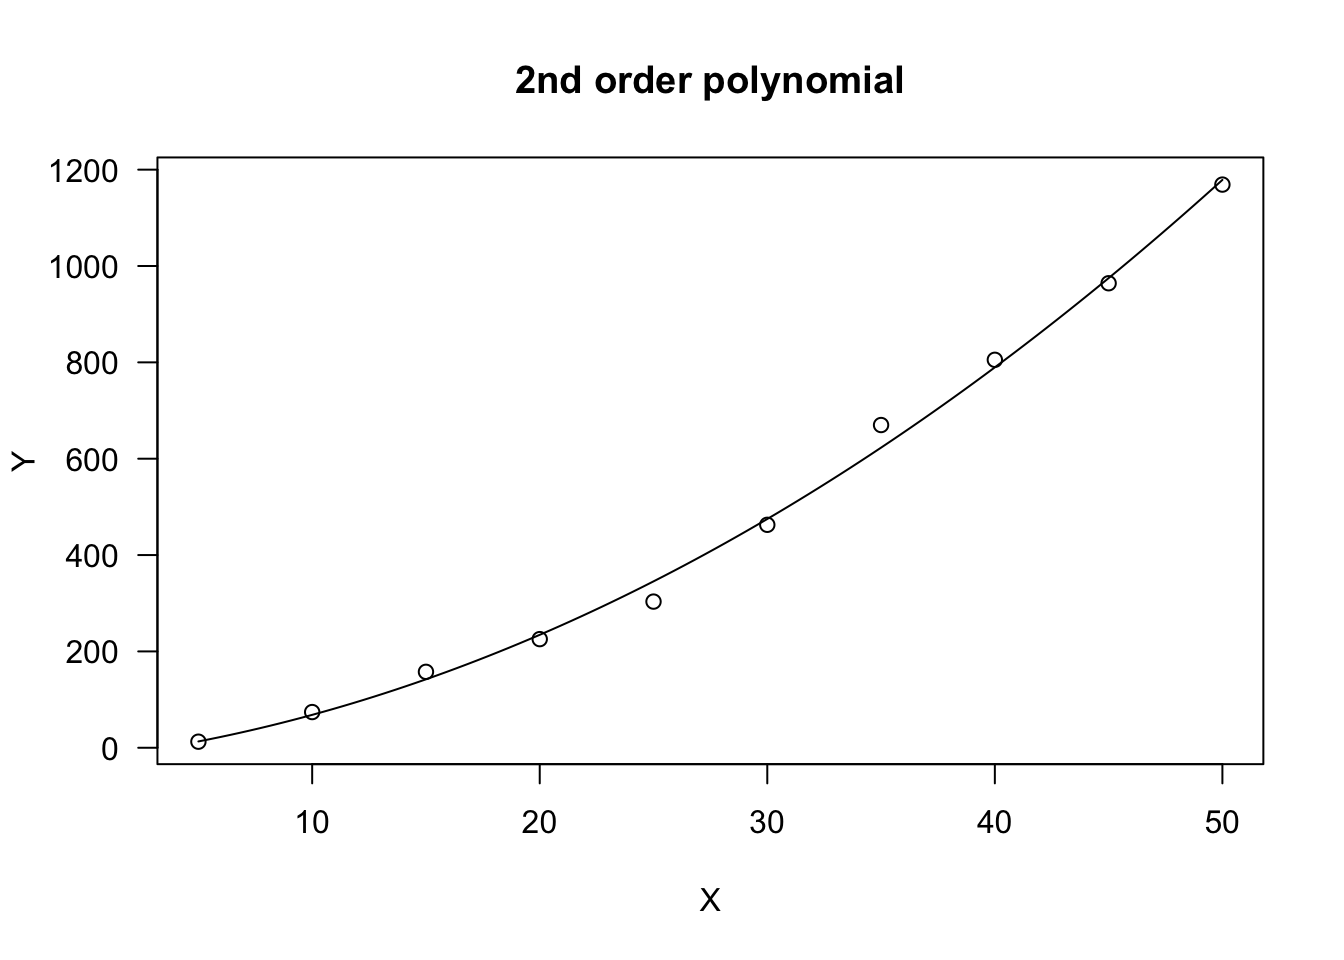
\includegraphics{_seedGerminationTutorial_files/figure-latex/unnamed-chunk-4-1.pdf}

What is the real germination time-course? The red one? The blue one? Something in between? We cannot really say this from our dataset, we are uncertain. The grey areas represent the uncertainty due to censoring. Do you think that we can reasonably neglect it?

\hypertarget{neglecting-censoring}{%
\section{Neglecting censoring}\label{neglecting-censoring}}

For a moment, let's forget about those grey uncertainty areas. Let's forget about censoring; this is what it is often done in literature for germination data: we associate the observed proportion of germinated seeds to the exact time when it was observed. It is, indeed, an abuse, as the observed data tell us a different story: the observed proportion of germinated seeds might have been attained before the moment of inspection (and not necessarily at the moment of inspection). But we disregard this and fit a nonlinear regression model, i.e.~a log-logistic function:

\[
G(t) = \frac{d}{ 1 + exp \left\{ - b \right[ \log(t) - \log(e) \left] \right\}}
\]

where \(G\) is the fraction of germinated seeds at time \(t\), \(d\) is the germinable fraction, \(e\) is the median germination time for the germinable fraction and \(b\) is the slope around the inflection point. The above model is sygmoidally shaped and it is symmetric on a log-time scale. The three parameters are biologically relevant, as they describe the three main features of seed germination, i.e.~capability (\(d\)), speed (\(e\)) and uniformity (\(b\)).

In order to fit a nonlinear regression model, we need to transform the observed data, as follows:

\begin{Shaded}
\begin{Highlighting}[]
\NormalTok{counts }\OtherTok{\textless{}{-}} \FunctionTok{as.numeric}\NormalTok{( }\FunctionTok{table}\NormalTok{( }\FunctionTok{cut}\NormalTok{(Gtimes, }\AttributeTok{breaks =} \FunctionTok{c}\NormalTok{(}\DecValTok{0}\NormalTok{, obsT)) ) )}
\NormalTok{propCum }\OtherTok{\textless{}{-}} \FunctionTok{cumsum}\NormalTok{(counts)}\SpecialCharTok{/}\DecValTok{100}
\NormalTok{df }\OtherTok{\textless{}{-}} \FunctionTok{data.frame}\NormalTok{(}\AttributeTok{time =}\NormalTok{ obsT, }\AttributeTok{counts =}\NormalTok{ counts, }\AttributeTok{propCum =}\NormalTok{ propCum) }
\NormalTok{df}
\DocumentationTok{\#\#    time counts propCum}
\DocumentationTok{\#\# 1     1      3    0.03}
\DocumentationTok{\#\# 2     2     11    0.14}
\DocumentationTok{\#\# 3     3     10    0.24}
\DocumentationTok{\#\# 4     4      8    0.32}
\DocumentationTok{\#\# 5     5     13    0.45}
\DocumentationTok{\#\# 6     6      2    0.47}
\DocumentationTok{\#\# 7     7      1    0.48}
\DocumentationTok{\#\# 8     8     12    0.60}
\DocumentationTok{\#\# 9     9      4    0.64}
\DocumentationTok{\#\# 10   10      5    0.69}
\DocumentationTok{\#\# 11   11      2    0.71}
\DocumentationTok{\#\# 12   12      3    0.74}
\DocumentationTok{\#\# 13   13      2    0.76}
\DocumentationTok{\#\# 14   14      2    0.78}
\DocumentationTok{\#\# 15   15      0    0.78}
\DocumentationTok{\#\# 16   16      1    0.79}
\DocumentationTok{\#\# 17   17      0    0.79}
\DocumentationTok{\#\# 18   18      0    0.79}
\DocumentationTok{\#\# 19   19      0    0.79}
\DocumentationTok{\#\# 20   20      1    0.80}
\DocumentationTok{\#\# 21   21      0    0.80}
\DocumentationTok{\#\# 22   22      1    0.81}
\DocumentationTok{\#\# 23   23      1    0.82}
\DocumentationTok{\#\# 24   24      0    0.82}
\DocumentationTok{\#\# 25   25      0    0.82}
\DocumentationTok{\#\# 26   26      0    0.82}
\DocumentationTok{\#\# 27   27      0    0.82}
\DocumentationTok{\#\# 28   28      1    0.83}
\DocumentationTok{\#\# 29   29      0    0.83}
\DocumentationTok{\#\# 30   30      0    0.83}
\DocumentationTok{\#\# 31   31      1    0.84}
\DocumentationTok{\#\# 32   32      1    0.85}
\DocumentationTok{\#\# 33   33      1    0.86}
\DocumentationTok{\#\# 34   34      0    0.86}
\DocumentationTok{\#\# 35   35      0    0.86}
\DocumentationTok{\#\# 36   36      0    0.86}
\DocumentationTok{\#\# 37   37      0    0.86}
\DocumentationTok{\#\# 38   38      0    0.86}
\DocumentationTok{\#\# 39   39      0    0.86}
\DocumentationTok{\#\# 40   40      0    0.86}
\end{Highlighting}
\end{Shaded}

In practice, we determine the cumulative proportion (or percentage) of germinated seeds (`propCum'), which is used as the response variable, while the observation time (`time') is used as the independent variable. Then, we fit the log-logistic function by non-linear least squares regression. I'll say this again: \textbf{you can clearly see that, by doing so, we totally neglect the grey areas in the figure above, we only look at the observed points}.

Let's use the `drm' function, in the `drc' package (Ritz et al., 2015). The argument `fct' is used to set the fitted function to log-logistic with three parameters (the equation above).

The \texttt{plot()} and \texttt{summary()} methods can be used to plot a graph and to retrieve the estimated parameters.

\begin{Shaded}
\begin{Highlighting}[]
\FunctionTok{library}\NormalTok{(drc)}
\NormalTok{mod }\OtherTok{\textless{}{-}} \FunctionTok{drm}\NormalTok{(propCum }\SpecialCharTok{\textasciitilde{}}\NormalTok{ time, }\AttributeTok{data =}\NormalTok{ df,}
           \AttributeTok{fct =} \FunctionTok{LL.3}\NormalTok{() )}
\FunctionTok{plot}\NormalTok{(mod, }\AttributeTok{log =} \StringTok{""}\NormalTok{,}
      \AttributeTok{xlab =} \StringTok{"Time (days)"}\NormalTok{,}
      \AttributeTok{ylab =} \StringTok{"Proportion of germinated seeds"}\NormalTok{)}
\end{Highlighting}
\end{Shaded}

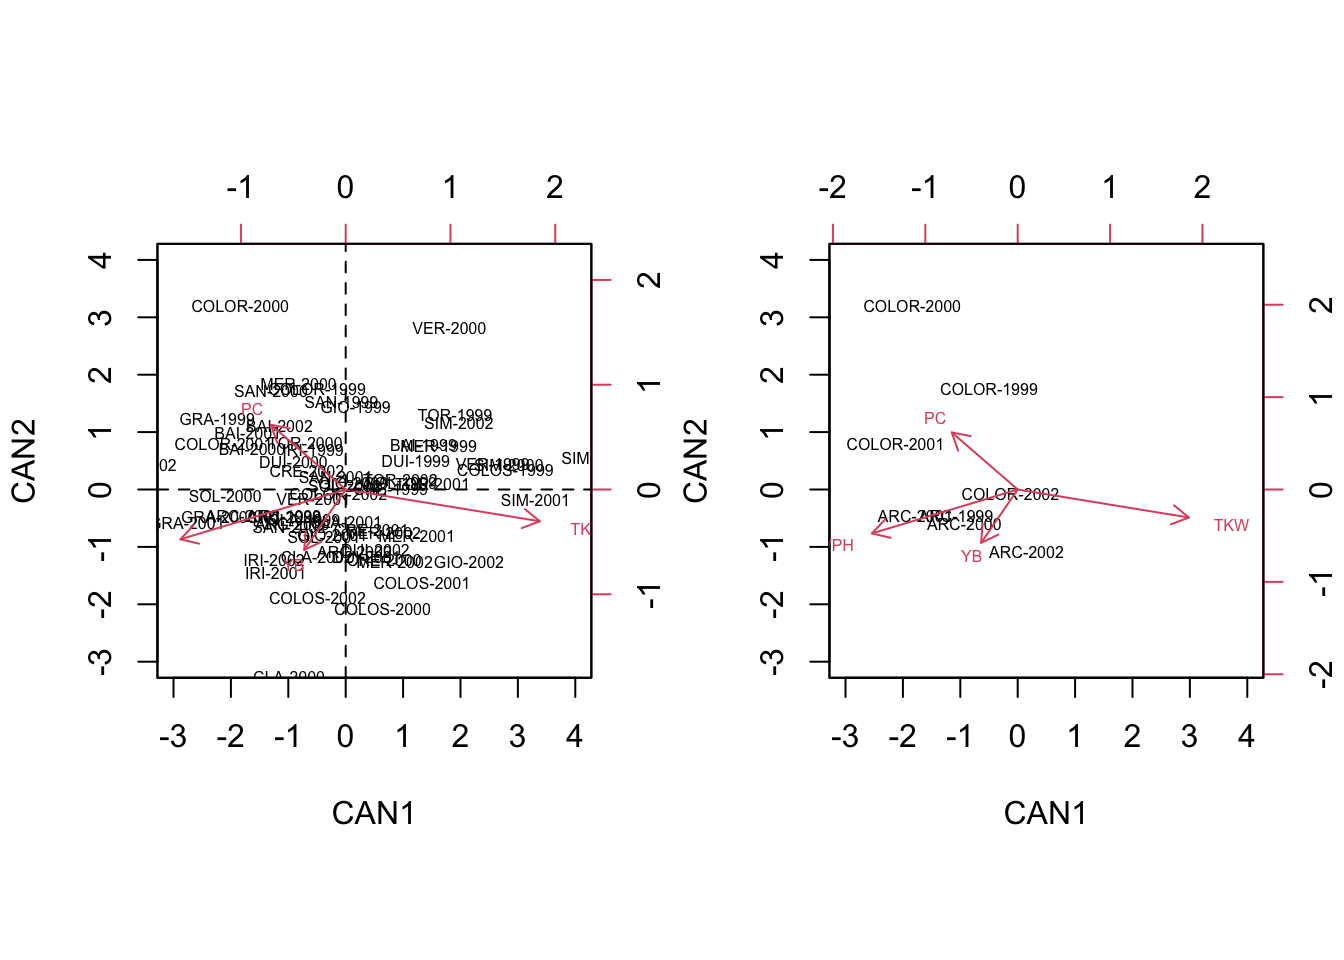
\includegraphics{_seedGerminationTutorial_files/figure-latex/unnamed-chunk-6-1.pdf}

\begin{Shaded}
\begin{Highlighting}[]
\FunctionTok{summary}\NormalTok{(mod)}
\DocumentationTok{\#\# }
\DocumentationTok{\#\# Model fitted: Log{-}logistic (ED50 as parameter) with lower limit at 0 (3 parms)}
\DocumentationTok{\#\# }
\DocumentationTok{\#\# Parameter estimates:}
\DocumentationTok{\#\# }
\DocumentationTok{\#\#                 Estimate Std. Error t{-}value   p{-}value    }
\DocumentationTok{\#\# b:(Intercept) {-}1.8497771  0.0702626 {-}26.327 \textless{} 2.2e{-}16 ***}
\DocumentationTok{\#\# d:(Intercept)  0.8768793  0.0070126 125.044 \textless{} 2.2e{-}16 ***}
\DocumentationTok{\#\# e:(Intercept)  5.2691575  0.1020457  51.635 \textless{} 2.2e{-}16 ***}
\DocumentationTok{\#\# {-}{-}{-}}
\DocumentationTok{\#\# Signif. codes:  0 \textquotesingle{}***\textquotesingle{} 0.001 \textquotesingle{}**\textquotesingle{} 0.01 \textquotesingle{}*\textquotesingle{} 0.05 \textquotesingle{}.\textquotesingle{} 0.1 \textquotesingle{} \textquotesingle{} 1}
\DocumentationTok{\#\# }
\DocumentationTok{\#\# Residual standard error:}
\DocumentationTok{\#\# }
\DocumentationTok{\#\#  0.01762168 (37 degrees of freedom)}
\end{Highlighting}
\end{Shaded}

We see that our estimates are very close to the real values (\(b\) = 1.85 vs.~1.6; \(e\) = 5.27 vs.~4.5; \(d\) = 0.88 vs.~0.86) and we also see that standard errors are rather small (the coefficient of variability goes from 1 to 4\%). There is a difference in sign for \(b\), which relates to the fact that the \texttt{LL.3()} function in `drc' removes the minus sign in the equation above. Please, disregard this aspect, which stems from the fact that the `drc' package is rooted in pesticide bioassays.

Do you think that this analysis is not that bad? Wait a moment. Let's see what happens if we account for censoring.

\hypertarget{accounting-for-censoring}{%
\section{Accounting for censoring}\label{accounting-for-censoring}}

How can we account for censoring? The answer is simple: we should use fitting methods which are specifically devised to incorporate the uncertainty due to censoring. We said that, in medicine, the body of these methods goes under the name of survival analysis and, from this framework, we can borrow a parametric survival model. However, I will not use the name `survival model' as we are not dealing with a survival process. Instead, I will use the name \textbf{parametric time-to-event model}.

My colleagues and I have extensively talked about parametric time-to-event models in two of our recent papers and related appendices (Onofri et al., 2019; Onofri et al., 2018). Therefore, I will not go into detail, now. I will just say that time-to-event models directly consider the observed counts as the response variable. As the independent variable, they consider the extremes of each time interval (`timeBef' and `timeAf'; see below). We immediately see two differences with nonlinear regression: (1) we do not need to transform the observed counts into cumulative proportions, and (2) by using an interval as the independent variable, we inject into the model the uncertainty due to censoring (the grey areas in the figure above). Let's reshape the dataset as shown below.

\begin{Shaded}
\begin{Highlighting}[]
\NormalTok{df }\OtherTok{\textless{}{-}} \FunctionTok{data.frame}\NormalTok{(}\AttributeTok{timeBef =} \FunctionTok{c}\NormalTok{(}\DecValTok{0}\NormalTok{, obsT), }\AttributeTok{timeAf =} \FunctionTok{c}\NormalTok{(obsT, }\ConstantTok{Inf}\NormalTok{), }\AttributeTok{counts =} \FunctionTok{c}\NormalTok{(}\FunctionTok{as.numeric}\NormalTok{(counts), }\DecValTok{100} \SpecialCharTok{{-}} \FunctionTok{sum}\NormalTok{(counts)) )}
\NormalTok{df}
\DocumentationTok{\#\#    timeBef timeAf counts}
\DocumentationTok{\#\# 1        0      1      3}
\DocumentationTok{\#\# 2        1      2     11}
\DocumentationTok{\#\# 3        2      3     10}
\DocumentationTok{\#\# 4        3      4      8}
\DocumentationTok{\#\# 5        4      5     13}
\DocumentationTok{\#\# 6        5      6      2}
\DocumentationTok{\#\# 7        6      7      1}
\DocumentationTok{\#\# 8        7      8     12}
\DocumentationTok{\#\# 9        8      9      4}
\DocumentationTok{\#\# 10       9     10      5}
\DocumentationTok{\#\# 11      10     11      2}
\DocumentationTok{\#\# 12      11     12      3}
\DocumentationTok{\#\# 13      12     13      2}
\DocumentationTok{\#\# 14      13     14      2}
\DocumentationTok{\#\# 15      14     15      0}
\DocumentationTok{\#\# 16      15     16      1}
\DocumentationTok{\#\# 17      16     17      0}
\DocumentationTok{\#\# 18      17     18      0}
\DocumentationTok{\#\# 19      18     19      0}
\DocumentationTok{\#\# 20      19     20      1}
\DocumentationTok{\#\# 21      20     21      0}
\DocumentationTok{\#\# 22      21     22      1}
\DocumentationTok{\#\# 23      22     23      1}
\DocumentationTok{\#\# 24      23     24      0}
\DocumentationTok{\#\# 25      24     25      0}
\DocumentationTok{\#\# 26      25     26      0}
\DocumentationTok{\#\# 27      26     27      0}
\DocumentationTok{\#\# 28      27     28      1}
\DocumentationTok{\#\# 29      28     29      0}
\DocumentationTok{\#\# 30      29     30      0}
\DocumentationTok{\#\# 31      30     31      1}
\DocumentationTok{\#\# 32      31     32      1}
\DocumentationTok{\#\# 33      32     33      1}
\DocumentationTok{\#\# 34      33     34      0}
\DocumentationTok{\#\# 35      34     35      0}
\DocumentationTok{\#\# 36      35     36      0}
\DocumentationTok{\#\# 37      36     37      0}
\DocumentationTok{\#\# 38      37     38      0}
\DocumentationTok{\#\# 39      38     39      0}
\DocumentationTok{\#\# 40      39     40      0}
\DocumentationTok{\#\# 41      40    Inf     14}
\end{Highlighting}
\end{Shaded}

Can you see the difference? Please, note that we also added the ungerminated seeds at the end, with an uncertainty interval going from 40 days to infinity.

Time-to-event models can be easily fitted by using the \texttt{drm()} function in the `drc' package, although we should specify that we want to use a time-to-event method, by setting the \texttt{type\ =\ "event"} argument. More simply, we can use the \texttt{drmte()} function in the `drcte' package, that is a specific package for time-to-event methods. Both the functions use the same syntax and, with respect to nonlinear regression, there are some important differences in the model call. In particular, a nonlinear regression model is defined as:

\begin{verbatim}
CumulativeProportion ~ timeAf
\end{verbatim}

On the other hand, a time-to-event model is defined as:

\begin{verbatim}
Count ~ timeBef + timeAf
\end{verbatim}

The full model call is shown below, both with \texttt{drm()} and with \texttt{drmte()}

\begin{Shaded}
\begin{Highlighting}[]
\CommentTok{\#Time{-}to{-}event model}
\FunctionTok{library}\NormalTok{(drcte)}
\CommentTok{\# modTE \textless{}{-} drm(counts \textasciitilde{} timeBef + timeAf, data = df, }
\CommentTok{\#            fct = LL.3(), type = "event")}
\NormalTok{modTE }\OtherTok{\textless{}{-}} \FunctionTok{drmte}\NormalTok{(counts }\SpecialCharTok{\textasciitilde{}}\NormalTok{ timeBef }\SpecialCharTok{+}\NormalTok{ timeAf, }\AttributeTok{data =}\NormalTok{ df, }
           \AttributeTok{fct =} \FunctionTok{LL.3}\NormalTok{())}
\FunctionTok{summary}\NormalTok{(modTE)}
\DocumentationTok{\#\# }
\DocumentationTok{\#\# Model fitted: Log{-}logistic (ED50 as parameter) with lower limit at 0}
\DocumentationTok{\#\# }
\DocumentationTok{\#\# Robust estimation: no }
\DocumentationTok{\#\# }
\DocumentationTok{\#\# Parameter estimates:}
\DocumentationTok{\#\# }
\DocumentationTok{\#\#                Estimate Std. Error t{-}value   p{-}value    }
\DocumentationTok{\#\# b:(Intercept) {-}1.826006   0.194579 {-}9.3844 \textless{} 2.2e{-}16 ***}
\DocumentationTok{\#\# d:(Intercept)  0.881476   0.036928 23.8701 \textless{} 2.2e{-}16 ***}
\DocumentationTok{\#\# e:(Intercept)  5.302109   0.565273  9.3797 \textless{} 2.2e{-}16 ***}
\DocumentationTok{\#\# {-}{-}{-}}
\DocumentationTok{\#\# Signif. codes:  0 \textquotesingle{}***\textquotesingle{} 0.001 \textquotesingle{}**\textquotesingle{} 0.01 \textquotesingle{}*\textquotesingle{} 0.05 \textquotesingle{}.\textquotesingle{} 0.1 \textquotesingle{} \textquotesingle{} 1}
\end{Highlighting}
\end{Shaded}

With respect to the nonlinear regression fit, the estimates from a time-to-event fit are very similar, but the standard errors are much higher (the coefficient of variability now goes from 4 to 11\%). That was expected: we have added the uncertainty due to censoring.

\hypertarget{neglecting-or-accounting-for-censoring}{%
\section{Neglecting or accounting for censoring?}\label{neglecting-or-accounting-for-censoring}}

You may wonder which of the two analysis is right and which is wrong. We cannot say this from just one dataset. However, we can repeat the Monte Carlo simulation above to extract 1000 samples, fit the model by using the two methods and retrieve parameter estimates and standard errors for each sample and method. We do this by using the code below (please, be patient\ldots{} it may take some time).

\begin{Shaded}
\begin{Highlighting}[]
\NormalTok{GermSampling }\OtherTok{\textless{}{-}} \ControlFlowTok{function}\NormalTok{(nSeeds, timeLast, stepOss, e, b, d)\{}
    
    \CommentTok{\#Draw a sample as above}
\NormalTok{    nGerm }\OtherTok{\textless{}{-}} \FunctionTok{rbinom}\NormalTok{(}\DecValTok{1}\NormalTok{, nSeeds, d)}
\NormalTok{    Gtimes }\OtherTok{\textless{}{-}} \FunctionTok{rllogis}\NormalTok{(nGerm, }\AttributeTok{shape =}\NormalTok{ b, }\AttributeTok{scale =}\NormalTok{ e)}
\NormalTok{    Gtimes }\OtherTok{\textless{}{-}} \FunctionTok{c}\NormalTok{(Gtimes, }\FunctionTok{rep}\NormalTok{(}\ConstantTok{Inf}\NormalTok{, }\DecValTok{100} \SpecialCharTok{{-}}\NormalTok{ nGerm))}

    
    \CommentTok{\#Generate the observed data}
\NormalTok{    obsT }\OtherTok{\textless{}{-}} \FunctionTok{seq}\NormalTok{(}\DecValTok{1}\NormalTok{, timeLast, }\AttributeTok{by=}\NormalTok{stepOss) }
\NormalTok{    counts }\OtherTok{\textless{}{-}} \FunctionTok{as.numeric}\NormalTok{( }\FunctionTok{table}\NormalTok{( }\FunctionTok{cut}\NormalTok{(Gtimes, }\AttributeTok{breaks =} \FunctionTok{c}\NormalTok{(}\DecValTok{0}\NormalTok{, obsT)) ) )}
\NormalTok{    propCum }\OtherTok{\textless{}{-}} \FunctionTok{cumsum}\NormalTok{(counts)}\SpecialCharTok{/}\NormalTok{nSeeds}
\NormalTok{    timeBef }\OtherTok{\textless{}{-}} \FunctionTok{c}\NormalTok{(}\DecValTok{0}\NormalTok{, obsT)}
\NormalTok{    timeAf }\OtherTok{\textless{}{-}} \FunctionTok{c}\NormalTok{(obsT, }\ConstantTok{Inf}\NormalTok{)}
\NormalTok{    counts }\OtherTok{\textless{}{-}} \FunctionTok{c}\NormalTok{(counts, nSeeds }\SpecialCharTok{{-}} \FunctionTok{sum}\NormalTok{(counts))}
    
    \CommentTok{\#Calculate the T50 with two methods}
\NormalTok{    mod }\OtherTok{\textless{}{-}} \FunctionTok{drm}\NormalTok{(propCum }\SpecialCharTok{\textasciitilde{}}\NormalTok{ obsT, }\AttributeTok{fct =} \FunctionTok{LL.3}\NormalTok{() )}
\NormalTok{    modTE }\OtherTok{\textless{}{-}} \FunctionTok{drm}\NormalTok{(counts }\SpecialCharTok{\textasciitilde{}}\NormalTok{ timeBef }\SpecialCharTok{+}\NormalTok{ timeAf, }
           \AttributeTok{fct =} \FunctionTok{LL.3}\NormalTok{(), }\AttributeTok{type =} \StringTok{"event"}\NormalTok{)}
    \FunctionTok{c}\NormalTok{(}\AttributeTok{b1 =} \FunctionTok{summary}\NormalTok{(mod)[[}\DecValTok{3}\NormalTok{]][}\DecValTok{1}\NormalTok{,}\DecValTok{1}\NormalTok{],}
      \AttributeTok{ESb1 =} \FunctionTok{summary}\NormalTok{(mod)[[}\DecValTok{3}\NormalTok{]][}\DecValTok{1}\NormalTok{,}\DecValTok{2}\NormalTok{],}
      \AttributeTok{b2 =} \FunctionTok{summary}\NormalTok{(modTE)[[}\DecValTok{3}\NormalTok{]][}\DecValTok{1}\NormalTok{,}\DecValTok{1}\NormalTok{],}
      \AttributeTok{ESb2 =} \FunctionTok{summary}\NormalTok{(modTE)[[}\DecValTok{3}\NormalTok{]][}\DecValTok{1}\NormalTok{,}\DecValTok{2}\NormalTok{],}
      \AttributeTok{d1 =} \FunctionTok{summary}\NormalTok{(mod)[[}\DecValTok{3}\NormalTok{]][}\DecValTok{2}\NormalTok{,}\DecValTok{1}\NormalTok{],}
      \AttributeTok{ESd1 =} \FunctionTok{summary}\NormalTok{(mod)[[}\DecValTok{3}\NormalTok{]][}\DecValTok{2}\NormalTok{,}\DecValTok{2}\NormalTok{],}
      \AttributeTok{d2 =} \FunctionTok{summary}\NormalTok{(modTE)[[}\DecValTok{3}\NormalTok{]][}\DecValTok{2}\NormalTok{,}\DecValTok{1}\NormalTok{],}
      \AttributeTok{ESd2 =} \FunctionTok{summary}\NormalTok{(modTE)[[}\DecValTok{3}\NormalTok{]][}\DecValTok{2}\NormalTok{,}\DecValTok{2}\NormalTok{],}
      \AttributeTok{e1 =} \FunctionTok{summary}\NormalTok{(mod)[[}\DecValTok{3}\NormalTok{]][}\DecValTok{3}\NormalTok{,}\DecValTok{1}\NormalTok{],}
      \AttributeTok{ESe1 =} \FunctionTok{summary}\NormalTok{(mod)[[}\DecValTok{3}\NormalTok{]][}\DecValTok{3}\NormalTok{,}\DecValTok{2}\NormalTok{],}
      \AttributeTok{e2 =} \FunctionTok{summary}\NormalTok{(modTE)[[}\DecValTok{3}\NormalTok{]][}\DecValTok{3}\NormalTok{,}\DecValTok{1}\NormalTok{],}
      \AttributeTok{ESe2 =} \FunctionTok{summary}\NormalTok{(modTE)[[}\DecValTok{3}\NormalTok{]][}\DecValTok{3}\NormalTok{,}\DecValTok{2}\NormalTok{] )}
\NormalTok{\}}

\FunctionTok{set.seed}\NormalTok{(}\DecValTok{1234}\NormalTok{)}
\NormalTok{result }\OtherTok{\textless{}{-}} \FunctionTok{data.frame}\NormalTok{()}
\ControlFlowTok{for}\NormalTok{ (i }\ControlFlowTok{in} \DecValTok{1}\SpecialCharTok{:}\DecValTok{1000}\NormalTok{) \{}
\NormalTok{  res }\OtherTok{\textless{}{-}} \FunctionTok{GermSampling}\NormalTok{(}\DecValTok{100}\NormalTok{, }\DecValTok{40}\NormalTok{, }\DecValTok{1}\NormalTok{, }\FloatTok{4.5}\NormalTok{, }\FloatTok{1.6}\NormalTok{, }\FloatTok{0.85}\NormalTok{)}
\NormalTok{  result }\OtherTok{\textless{}{-}} \FunctionTok{rbind}\NormalTok{(result, res)}
\NormalTok{\} }
\FunctionTok{names}\NormalTok{(result) }\OtherTok{\textless{}{-}} \FunctionTok{c}\NormalTok{(}\StringTok{"b1"}\NormalTok{, }\StringTok{"ESb1"}\NormalTok{, }\StringTok{"b2"}\NormalTok{, }\StringTok{"ESb2"}\NormalTok{,}
                   \StringTok{"d1"}\NormalTok{, }\StringTok{"ESd1"}\NormalTok{, }\StringTok{"d2"}\NormalTok{, }\StringTok{"ESd2"}\NormalTok{,}
                   \StringTok{"e1"}\NormalTok{, }\StringTok{"ESe1"}\NormalTok{, }\StringTok{"e2"}\NormalTok{, }\StringTok{"ESe2"}\NormalTok{)}
\NormalTok{result }\OtherTok{\textless{}{-}}\NormalTok{ result[result}\SpecialCharTok{$}\NormalTok{d2 }\SpecialCharTok{\textgreater{}} \DecValTok{0}\NormalTok{,]}
\end{Highlighting}
\end{Shaded}

We have stored our results in the data frame `result'. The means of estimates obtained for both methods should be equal to the real values that we used for the simulation, which will ensure that estimators are unbiased. The means of standard errors (in brackets, below) should represent the real sample-to-sample variability, which may be obtained from the Monte Carlo standard deviation, i.e.~from the standard deviation of the 1000 estimates for each parameter and method.

\begin{tabular}{l|l|l|l}
\hline
  & \$b\$ & \$d\$ & \$e\$\\
\hline
Nonlinear regression & 1.63 (0.051) & 0.85 (0.006) & 4.55 (0.086)\\
\hline
Time-to-event method & 1.62 (0.187) & 0.85 (0.041) & 4.55 (0.579)\\
\hline
Real values & 1.60 (0.188) & 0.85 (0.041) & 4.55 (0.593)\\
\hline
\end{tabular}

We clearly see that both nonlinear regression and the time-to-event method lead to unbiased estimates of model parameters. However, standard errors from nonlinear regression are severely biased and underestimated. On the contrary, standard errors from time-to-event method are unbiased.

\hypertarget{take-home-message}{%
\section{Take-home message}\label{take-home-message}}

Censoring is peculiar to germination assays and other time-to-event studies. It may have a strong impact on the reliability of our standard errors and, consequently, on hypotheses testing. Therefore, censoring should never be neglected and time-to-event methods should necessarily be used for data analyses. The body of time-to-event methods often goes under the name of `survival analysis', which creates a direct connection between survival data and germination/emergence data.

\hypertarget{reshaping-time-to-event-data}{%
\chapter{Reshaping time-to-event data}\label{reshaping-time-to-event-data}}

Let's now open a parenthesis about the structure of germination/emergence data. To our experience, seed scientists are used to storing their datasets in several formats, that may not be immediately usable with the `drcte' and `drc' packages, which this tutorial is built upon. The figure below shows some of the possible formats that I have often encountered in my consulting work.

\begin{figure}

{\centering 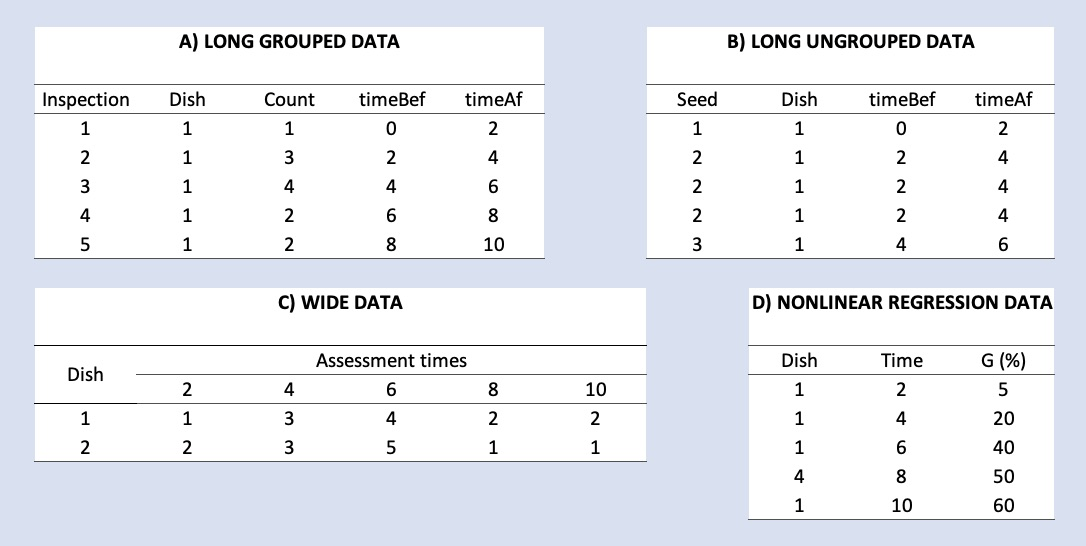
\includegraphics[width=0.9\linewidth]{_Figures/Stat_drcte_3-method-data} 

}

\caption{Possible data structures for seed germination/emergence data}\label{fig:figName2}
\end{figure}

Both the `drcte' and `drc' packages require that the data is stored in LONG GROUPED format, as shown in the figure above (panel A, top left). We have already mentioned in the previous section that each row represents a time interval, the columns `timeBef' and `timeAf' represent the beginning and ending of the interval, while the column `count' represents the seeds that germinated/emerged during that interval of time. Other columns may be needed, to represent, e.g., the randomisation unit (e.g., Petri dish) within which the count was made and the experimental treatment level that was allocated to that unit.

Apart from the LONG GROUPED format, other time-to-event packages, such as `survival' (Therneau, 2021) or `interval' (Fay and Shaw, 2010) require a different data format, which could be named as LONG UNGROUPED (Figure above, panel B, top right). In this format, each row represents a seed, while the columns `timeBef' and `timeAf' represent the beginning and ending of the interval during which that seed germinated/emerged. The column `count' is not necessary, while other columns may be necessary, as for the LONG GROUPED format. Apart from the above mentioned `survival' and `interval' packages, this format is also compatible with the `drcte' package.

Both the GROUPED and UNGROUPED formats have two basic advantages: (i) they can be used with all types of time-to-event data and (ii) they obey to the principles of tidy data (Wickham, 2016). However, to my experience, seed scientists often use other formats, such as the WIDE format (Figure above, panel C, bottom left) or the NONLINEAR REGRESSION format (Figure above, panel D, bottom right), which need to be preliminary transformed into one of the LONG GROUPED or LONG UNGROUPED formats.

In order to ease the transition from traditional methods of data analysis to time-to-event methods, we decided to develop a couple of service functions that can be used to reshape the data to a format that is more suitable for time-to-event analyses. Let's see how to do this by using a `real-life' example.

\hypertarget{motivating-example}{%
\section{Motivating example}\label{motivating-example}}

Seeds of \emph{L. ornithopodioides} were collected from natural populations, at three different maturation stages, i.e.~at 27 Days After Anthesis (DAA), when seeds were still green (Stage A), at 35 DAA, when seeds were brown and soft (Stage B) and at 41 DAA, when seeds were brown and moderately hard (Stage C). Germination assays were performed by placing four replicates of 25 seeds on filter paper (Whatman no. 3) in 9-cm diameter Petri dishes, in the dark and at a constant temperature of 20°C. The filter paper was initially moistened with 5 mL of distilled water and replenished as needed during the assay. Germinated seeds were counted daily over 15 days and removed from the Petri dishes. This dataset is a subset of a bigger dataset, aimed at assessing the time when the hard coat imposes dormancy in seeds of different legume species (Gresta et al., 2011).

The authors of the above study sent me the above dataset in WIDE format, where the rows represented each Petri dish and the columns represented all information about each dish, including the counts of germinated seeds, which were listed in different columns. The dataset is shown in the table below and it is available as the `lotusOr' dataframe in the `drcte' package.

\begin{verbatim}
##  Stage Dish 1  2 3 4 5 6 7 8 9 10 11 12 13 14 15
##      A    1 0  0 0 0 0 1 2 1 1  1  3  1  1  4  2
##      A    2 0  0 0 0 0 1 1 1 1  2  1  2  3  1  1
##      A    3 0  0 0 0 0 3 4 4 3  1  2  1  1  0  1
##      A    4 0  0 0 0 0 1 3 1 2  1  2  1  3  1  1
##      B    5 0  0 0 4 1 2 1 1 0  1  2  2  3  2  1
##      B    6 0  0 0 4 2 2 1 0 1  1  3  4  3  4  0
##      B    7 0  0 0 4 0 4 1 2 1  1  3  3  2  2  0
##      B    8 0  0 0 4 3 2 2 3 1  1  1  1  1  0  0
##      C    9 1 10 1 2 1 2 3 2 0  0  0  0  1  0  0
##      C   10 1 10 4 1 4 0 1 1 0  0  0  0  1  0  1
##      C   11 1 11 5 1 2 2 1 0 1  0  0  1  0  0  0
##      C   12 0 16 1 2 2 1 1 0 0  1  0  0  0  1  0
\end{verbatim}

The WIDE format is handy for swift calculations with a spreadsheet, but, in general, it is not ok, as: (1) it does not obey to the principle of tidy data (Wickham, 2016); (2) it is not generally efficient and it cannot be used with a set of germination assays with different monitoring schedules. Therefore, facing a dataset in the WIDE format, we need to reshape it into a LONG format.

\hypertarget{transforming-from-wide-to-long-grouped}{%
\section{Transforming from WIDE to LONG GROUPED}\label{transforming-from-wide-to-long-grouped}}

For such a reshaping, we could use one of the available R functions, such us \texttt{pivot\_longer()} in the `tidyverse' or \texttt{melt()} in the `reshape' package. However, when reshaping the data, it is also useful to make e few transformations, such as producing cumulative counts and proportions, that might be useful to plot graphs, or for other purposes. Therefore, we developed the \texttt{melt\_te()} function; let's look at its usage, in the box below.

\begin{Shaded}
\begin{Highlighting}[]
\NormalTok{datasetG }\OtherTok{\textless{}{-}} \FunctionTok{melt\_te}\NormalTok{(lotusOr, }\AttributeTok{count\_cols =} \DecValTok{3}\SpecialCharTok{:}\DecValTok{17}\NormalTok{, }\AttributeTok{treat =}\NormalTok{ Stage, }
                   \AttributeTok{monitimes =} \DecValTok{1}\SpecialCharTok{:}\DecValTok{15}\NormalTok{, }\AttributeTok{n.subjects =} \FunctionTok{rep}\NormalTok{(}\DecValTok{25}\NormalTok{,}\DecValTok{12}\NormalTok{))}
\FunctionTok{head}\NormalTok{(datasetG, }\DecValTok{16}\NormalTok{)}
\DocumentationTok{\#\#    Stage Units timeBef timeAf count nCum propCum}
\DocumentationTok{\#\# 1      A     1       0      1     0    0    0.00}
\DocumentationTok{\#\# 2      A     1       1      2     0    0    0.00}
\DocumentationTok{\#\# 3      A     1       2      3     0    0    0.00}
\DocumentationTok{\#\# 4      A     1       3      4     0    0    0.00}
\DocumentationTok{\#\# 5      A     1       4      5     0    0    0.00}
\DocumentationTok{\#\# 6      A     1       5      6     1    1    0.04}
\DocumentationTok{\#\# 7      A     1       6      7     2    3    0.12}
\DocumentationTok{\#\# 8      A     1       7      8     1    4    0.16}
\DocumentationTok{\#\# 9      A     1       8      9     1    5    0.20}
\DocumentationTok{\#\# 10     A     1       9     10     1    6    0.24}
\DocumentationTok{\#\# 11     A     1      10     11     3    9    0.36}
\DocumentationTok{\#\# 12     A     1      11     12     1   10    0.40}
\DocumentationTok{\#\# 13     A     1      12     13     1   11    0.44}
\DocumentationTok{\#\# 14     A     1      13     14     4   15    0.60}
\DocumentationTok{\#\# 15     A     1      14     15     2   17    0.68}
\DocumentationTok{\#\# 16     A     1      15    Inf     8   NA      NA}
\end{Highlighting}
\end{Shaded}

The \texttt{melt\_te()} function requires the following arguments:

\begin{enumerate}
\def\labelenumi{\arabic{enumi}.}
\tightlist
\item
  data: the original dataframe
\item
  count\_cols: the positions of the columns in `data', listing, for each dish, the counts of germinated seeds at each assessment time (columns)
\item
  treat: the columns in `data', listing, for each dish, the levels of each experimental treatment
\item
  monitimes: a vector of monitoring times that needs to be of the same length as the argument `count\_cols'
\item
  subjects: a vector with the number of viable seeds per dish, at the beginning of the assay. If this argument is omitted, the function assumes that such a number is equal to the total count of germinated seeds in each dish
\end{enumerate}

The functions outputs a dataframe in LONG format, where the initial columns code for the experimental treatments, the column `Units' represents the original rows (Petri dishes), `timeAf' represents the time at which the observation was made, `timeBef' represents the time at which the previous observation was made, `count' represents the number of seeds that germinated between `timeBef' and `timeAf', `nCum' is the cumulative count and `propCum' is the cumulative proportion of germinated seeds. An extra row is added for the ungerminated seeds at the end of the assay, with `timeBef' equal to the final assessment time and `timeAf' equal to \(\infty\).

\hypertarget{transforming-from-wide-to-long-ungrouped}{%
\section{Transforming from WIDE to LONG UNGROUPED}\label{transforming-from-wide-to-long-ungrouped}}

The LONG GROUPED format is good for the packages `drc' and `drcte'. However, we might be interested in performing data analyses within the framework of survival analysis, e.g.~with the `survival' or `interval' packages, that require the LONG UNGROUPED format. In order to reshape the original dataset into the LONG UNGROUPED format, we can use the same \texttt{melt\_te()} function, by setting the argument \texttt{grouped\ =\ FALSE}. An example is given in the box below.

\begin{Shaded}
\begin{Highlighting}[]
\NormalTok{datasetU }\OtherTok{\textless{}{-}} \FunctionTok{melt\_te}\NormalTok{(lotusOr, }\AttributeTok{count\_cols =} \DecValTok{3}\SpecialCharTok{:}\DecValTok{17}\NormalTok{, }\AttributeTok{treat =} \DecValTok{1}\NormalTok{, }
                   \AttributeTok{monitimes =} \DecValTok{1}\SpecialCharTok{:}\DecValTok{15}\NormalTok{, }\AttributeTok{n.subjects =} \FunctionTok{rep}\NormalTok{(}\DecValTok{25}\NormalTok{,}\DecValTok{12}\NormalTok{), }\AttributeTok{grouped =}\NormalTok{ F)}
\FunctionTok{head}\NormalTok{(datasetU, }\DecValTok{16}\NormalTok{)}
\DocumentationTok{\#\#    Stage Units timeBef timeAf}
\DocumentationTok{\#\# 1      A     1       5      6}
\DocumentationTok{\#\# 2      A     1       6      7}
\DocumentationTok{\#\# 3      A     1       6      7}
\DocumentationTok{\#\# 4      A     1       7      8}
\DocumentationTok{\#\# 5      A     1       8      9}
\DocumentationTok{\#\# 6      A     1       9     10}
\DocumentationTok{\#\# 7      A     1      10     11}
\DocumentationTok{\#\# 8      A     1      10     11}
\DocumentationTok{\#\# 9      A     1      10     11}
\DocumentationTok{\#\# 10     A     1      11     12}
\DocumentationTok{\#\# 11     A     1      12     13}
\DocumentationTok{\#\# 12     A     1      13     14}
\DocumentationTok{\#\# 13     A     1      13     14}
\DocumentationTok{\#\# 14     A     1      13     14}
\DocumentationTok{\#\# 15     A     1      13     14}
\DocumentationTok{\#\# 16     A     1      14     15}
\end{Highlighting}
\end{Shaded}

\hypertarget{from-long-grouped-to-long-ungrouped-and-vice-versa}{%
\section{From LONG GROUPED to LONG UNGROUPED (and vice-versa)}\label{from-long-grouped-to-long-ungrouped-and-vice-versa}}

If necessary, we can easily reshape back and forth from the GROUPED and UNGROUPED formats, by using the funtions \texttt{ungroup\_te} and \texttt{group\_te()}. See the sample code below.

\begin{Shaded}
\begin{Highlighting}[]
\CommentTok{\# From LONG GROUPED to LONG UNGROUPED}
\NormalTok{datasetU2 }\OtherTok{\textless{}{-}} \FunctionTok{ungroup\_te}\NormalTok{(datasetG, count)[,}\SpecialCharTok{{-}}\FunctionTok{c}\NormalTok{(}\DecValTok{5}\NormalTok{, }\DecValTok{6}\NormalTok{)]}
\FunctionTok{head}\NormalTok{(datasetU2, }\DecValTok{16}\NormalTok{)}
\DocumentationTok{\#\#    Stage Units timeBef timeAf}
\DocumentationTok{\#\# 1      A     1       5      6}
\DocumentationTok{\#\# 2      A     1       6      7}
\DocumentationTok{\#\# 3      A     1       6      7}
\DocumentationTok{\#\# 4      A     1       7      8}
\DocumentationTok{\#\# 5      A     1       8      9}
\DocumentationTok{\#\# 6      A     1       9     10}
\DocumentationTok{\#\# 7      A     1      10     11}
\DocumentationTok{\#\# 8      A     1      10     11}
\DocumentationTok{\#\# 9      A     1      10     11}
\DocumentationTok{\#\# 10     A     1      11     12}
\DocumentationTok{\#\# 11     A     1      12     13}
\DocumentationTok{\#\# 12     A     1      13     14}
\DocumentationTok{\#\# 13     A     1      13     14}
\DocumentationTok{\#\# 14     A     1      13     14}
\DocumentationTok{\#\# 15     A     1      13     14}
\DocumentationTok{\#\# 16     A     1      14     15}
\end{Highlighting}
\end{Shaded}

\begin{Shaded}
\begin{Highlighting}[]
\CommentTok{\# From LONG UNGROUPED to LONG GROUPED}
\NormalTok{datasetG2 }\OtherTok{\textless{}{-}} \FunctionTok{group\_te}\NormalTok{(datasetU)}
\FunctionTok{head}\NormalTok{(datasetG2, }\DecValTok{16}\NormalTok{)}
\DocumentationTok{\#\#    Stage Units timeBef timeAf count}
\DocumentationTok{\#\# 1      A     1       5      6     1}
\DocumentationTok{\#\# 2      A     1       6      7     2}
\DocumentationTok{\#\# 3      A     1       7      8     1}
\DocumentationTok{\#\# 4      A     1       8      9     1}
\DocumentationTok{\#\# 5      A     1       9     10     1}
\DocumentationTok{\#\# 6      A     1      10     11     3}
\DocumentationTok{\#\# 7      A     1      11     12     1}
\DocumentationTok{\#\# 8      A     1      12     13     1}
\DocumentationTok{\#\# 9      A     1      13     14     4}
\DocumentationTok{\#\# 10     A     1      14     15     2}
\DocumentationTok{\#\# 11     A     1      15    Inf     8}
\DocumentationTok{\#\# 12     A     2       5      6     1}
\DocumentationTok{\#\# 13     A     2       6      7     1}
\DocumentationTok{\#\# 14     A     2       7      8     1}
\DocumentationTok{\#\# 15     A     2       8      9     1}
\DocumentationTok{\#\# 16     A     2       9     10     2}
\end{Highlighting}
\end{Shaded}

\hypertarget{from-nonlinear-regression-to-long-grouped}{%
\section{From NONLINEAR REGRESSION to LONG GROUPED}\label{from-nonlinear-regression-to-long-grouped}}

In other instances, it may happen that the dataset was prepared as required by nonlinear regression analysis, i.e.~listing the cumulative number of germinated seeds at each inspection time. The following Table shows an example for the first Petri dish, as available in the `lotusCum' dataframe in the `drcte' package.

\begin{verbatim}
##  Stage Dish Time nCum
##      A    1    1    0
##      A    1    2    0
##      A    1    3    0
##      A    1    4    0
##      A    1    5    0
##      A    1    6    1
##      A    1    7    3
##      A    1    8    4
##      A    1    9    5
##      A    1   10    6
##      A    1   11    9
##      A    1   12   10
##      A    1   13   11
##      A    1   14   15
##      A    1   15   17
\end{verbatim}

In this situation, we need to `decumulate' the counts and add the beginning of each inspection interval (e.g., `timeBef'). We can easily do this by using the \texttt{decumulate\_te()} function in `drcte'. An example is given in the box below.

\begin{Shaded}
\begin{Highlighting}[]
\NormalTok{dataset\_sd }\OtherTok{\textless{}{-}} \FunctionTok{decumulate\_te}\NormalTok{(lotusCum,}
                            \AttributeTok{resp =}\NormalTok{ nCum, }
                            \AttributeTok{treat =}\NormalTok{ Stage,}
                            \AttributeTok{monitimes =}\NormalTok{ Time,}
                            \AttributeTok{units =}\NormalTok{ Dish, }
                            \AttributeTok{n.subjects =} \FunctionTok{rep}\NormalTok{(}\DecValTok{25}\NormalTok{, }\DecValTok{12}\NormalTok{),}
                            \AttributeTok{type =} \StringTok{"count"}\NormalTok{)}
\NormalTok{dataset\_sd }\OtherTok{\textless{}{-}} \FunctionTok{decumulate\_te}\NormalTok{(lotusCum,}
                            \AttributeTok{resp =}\NormalTok{ Prop, }
                            \AttributeTok{treat =}\NormalTok{ Stage,}
                            \AttributeTok{monitimes =}\NormalTok{ Time,}
                            \AttributeTok{units =}\NormalTok{ Dish, }
                            \AttributeTok{n.subjects =} \FunctionTok{rep}\NormalTok{(}\DecValTok{25}\NormalTok{, }\DecValTok{12}\NormalTok{),}
                            \AttributeTok{type =} \StringTok{"proportion"}\NormalTok{)}
\end{Highlighting}
\end{Shaded}

The \texttt{decumulate\_te()} function requires the following arguments:

\begin{enumerate}
\def\labelenumi{\arabic{enumi}.}
\tightlist
\item
  resp: the column containing the counts/proportions of germinated seeds
\item
  treat: the columns listing, for each row of data, the corresponding level of experimental factors (one factor per column)
\item
  monitimes: the column listing monitoring times
\item
  units: the column listing the randomisation units
\item
  subjects: a vector listing the number of viable seeds, at the beginning of the assay, for each randomisation unit.
\item
  type: a value specifying if `resp' contains `counts' or `proportions'
\end{enumerate}

We do hope that, with these functions, we can menage to ease your transition from traditional methods of data analysis to time-to-event methods, for seed germination/emergence assays.

\hypertarget{time-to-event-models-for-seed-germinationemergence}{%
\chapter{Time-to-event models for seed germination/emergence}\label{time-to-event-models-for-seed-germinationemergence}}

The individual seeds within a population do not germinate/emerge altogether at the same moment; this is an undisputed fact, resulting from seed-to-seed variability in germination/emergence time. Accordingly, the primary reason why we organise germination assays is to describe the progress to germination for the whole population, by using some appropriate time-to-event model.

What is a time-to-event model? It is a model that describes the probability that the event (germination/emergence, in our case) occurs at any time \(t\) or before that time:

\[ P(t) = \Phi(T \le t)\]

In practice, it may be easier to think that \(P(t)\) is the proportion of germinated/emerged seeds at time \(t\). In statistical terms, \(\Phi\) is a Cumulative Distribution Function (CDF), with the following characteristics:

\begin{enumerate}
\def\labelenumi{\arabic{enumi}.}
\tightlist
\item
  the time \(t\) is constrained from 0 to +\(\infty\)
\item
  the response \(P(t)\) is constrained from 0 to 1
\item
  the response \(P(t)\) is monotonically increasing
\item
  due to the possible presence of a final fraction of individuals without the event (e.g., ungerminated seeds), \(P(t)\) may not necessarily reach 1.
\end{enumerate}

The first task to fit a time-to-event model is to select a form for \(\Phi\). In general, we have three possibilities:

\begin{enumerate}
\def\labelenumi{\arabic{enumi}.}
\tightlist
\item
  a parametric maximum likelihood model (ML)
\item
  a non-parametric maximum likelihood model (NPMLE)
\item
  a kernel density estimator (KDE)
\end{enumerate}

Let's have a closer look at those three options.

\hypertarget{parametric-time-to-event-models}{%
\section{Parametric time-to-event models}\label{parametric-time-to-event-models}}

The CDF for parametric time-to-event models is characterised by a pre-defined, usually sigmoidal, shape. Right-skewed CDFs have proven useful, such as the log-normal, log-logistic or Weibull, which are only defined for \(t > 0\) (see \#1 above). These CDFs contain a location (\(e\)) and a scale (\(b\)) parameter: the former is a measure of central tendency (e.g., the median for the log-logistic and log-normal CDFs) while the latter is a measure of how fast the curve grows during time. For seed germination/emergence, most often, a third parameter is necessary, to describe the fraction of dormant or nonviable seeds (\(0 < d \leq 1\)). As an example, we show a log-logistic CDF, that is also used in ecotoxicology, for dose-response studies:

\[P(t) = \frac{d}{1 + exp\left\{ b \right[ \log(t) - log(e)\left] \right\}}\]

Fitting the above parametric model implies that, based on the observed data, we need to assign a specific value to the parameters \(b\), \(d\) and \(e\), so that an appropriate likelihood function is maximised (Maximum Likelihood estimation). Relating to the estimation process, we should necessarily take into account that germination/emergence data are censored data; neglecting this fact has some important consequences, as I have described \href{https://www.statforbiology.com/2021/stat_drcte_2-methods/}{in this post}.

In practice, parametric time-to-event models can be fitted by the \texttt{drmte()} function in the `drcte' package. As an example, let's consider a factitious dataset relating to an assay where the germinations of 30 seeds were counted daily for 15 days. A log-logistic time-to-event model can be easily fit as follows:

\begin{Shaded}
\begin{Highlighting}[]
\NormalTok{dataset }\OtherTok{\textless{}{-}} \FunctionTok{read.csv}\NormalTok{(}\StringTok{"https://www.casaonofri.it/\_datasets/oneFlush.csv"}\NormalTok{)}
\FunctionTok{head}\NormalTok{(dataset)}
\DocumentationTok{\#\#   timeBef timeAf counts}
\DocumentationTok{\#\# 1       0      1      3}
\DocumentationTok{\#\# 2       1      2      2}
\DocumentationTok{\#\# 3       2      3      3}
\DocumentationTok{\#\# 4       3      4      4}
\DocumentationTok{\#\# 5       4      5      3}
\DocumentationTok{\#\# 6       5      6      2}
\FunctionTok{library}\NormalTok{(drcte)}
\NormalTok{te.mod }\OtherTok{\textless{}{-}} \FunctionTok{drmte}\NormalTok{(counts }\SpecialCharTok{\textasciitilde{}}\NormalTok{ timeBef }\SpecialCharTok{+}\NormalTok{ timeAf, }\AttributeTok{fct =} \FunctionTok{LL.3}\NormalTok{(),}
                \AttributeTok{data =}\NormalTok{ dataset)}
\CommentTok{\# Alternative}
\CommentTok{\# te.mod \textless{}{-} drm(counts \textasciitilde{} timeBef + timeAf, fct = LL.3(),}
\CommentTok{\#                 data = dataset, type = "event")}
\end{Highlighting}
\end{Shaded}

We can see that we have directly considered the observed counts as the response variable, with no preliminary transformation. Furthermore, we have two predictors that represent the extremes of each time interval (`timeBef' and `timeAf'), by which we associate each count to the whole uncertainty interval during which germinations took place and not to a precise time instant. In other words, we fully respect our censored data.

The very same model can be fitted by using the \texttt{drm()} function in the `drc' package, although we should add the argument \texttt{type\ =\ "event"}, as this latter package is not specific to time-to-event methods.

The usual \texttt{coef()}, \texttt{summary()}, \texttt{print()} and \texttt{plot()} methods can be used for `drcte' objects as for any other model object in R.

\begin{Shaded}
\begin{Highlighting}[]
\FunctionTok{summary}\NormalTok{(te.mod)}
\DocumentationTok{\#\# }
\DocumentationTok{\#\# Model fitted: Log{-}logistic (ED50 as parameter) with lower limit at 0}
\DocumentationTok{\#\# }
\DocumentationTok{\#\# Robust estimation: no }
\DocumentationTok{\#\# }
\DocumentationTok{\#\# Parameter estimates:}
\DocumentationTok{\#\# }
\DocumentationTok{\#\#               Estimate Std. Error t{-}value   p{-}value    }
\DocumentationTok{\#\# b:(Intercept) {-}1.52553    0.44166 {-}3.4541 0.0005521 ***}
\DocumentationTok{\#\# d:(Intercept)  0.97842    0.16027  6.1048  1.03e{-}09 ***}
\DocumentationTok{\#\# e:(Intercept)  4.91400    1.68058  2.9240 0.0034558 ** }
\DocumentationTok{\#\# {-}{-}{-}}
\DocumentationTok{\#\# Signif. codes:  0 \textquotesingle{}***\textquotesingle{} 0.001 \textquotesingle{}**\textquotesingle{} 0.01 \textquotesingle{}*\textquotesingle{} 0.05 \textquotesingle{}.\textquotesingle{} 0.1 \textquotesingle{} \textquotesingle{} 1}
\FunctionTok{plot}\NormalTok{(te.mod, }\AttributeTok{ylim =} \FunctionTok{c}\NormalTok{(}\DecValTok{0}\NormalTok{, }\DecValTok{1}\NormalTok{), }\AttributeTok{xlim =} \FunctionTok{c}\NormalTok{(}\DecValTok{0}\NormalTok{, }\DecValTok{15}\NormalTok{),}
     \AttributeTok{xlab =} \StringTok{"Time"}\NormalTok{, }\AttributeTok{ylab =} \StringTok{"Cumulative proportion of germinated seeds"}\NormalTok{)}
\end{Highlighting}
\end{Shaded}

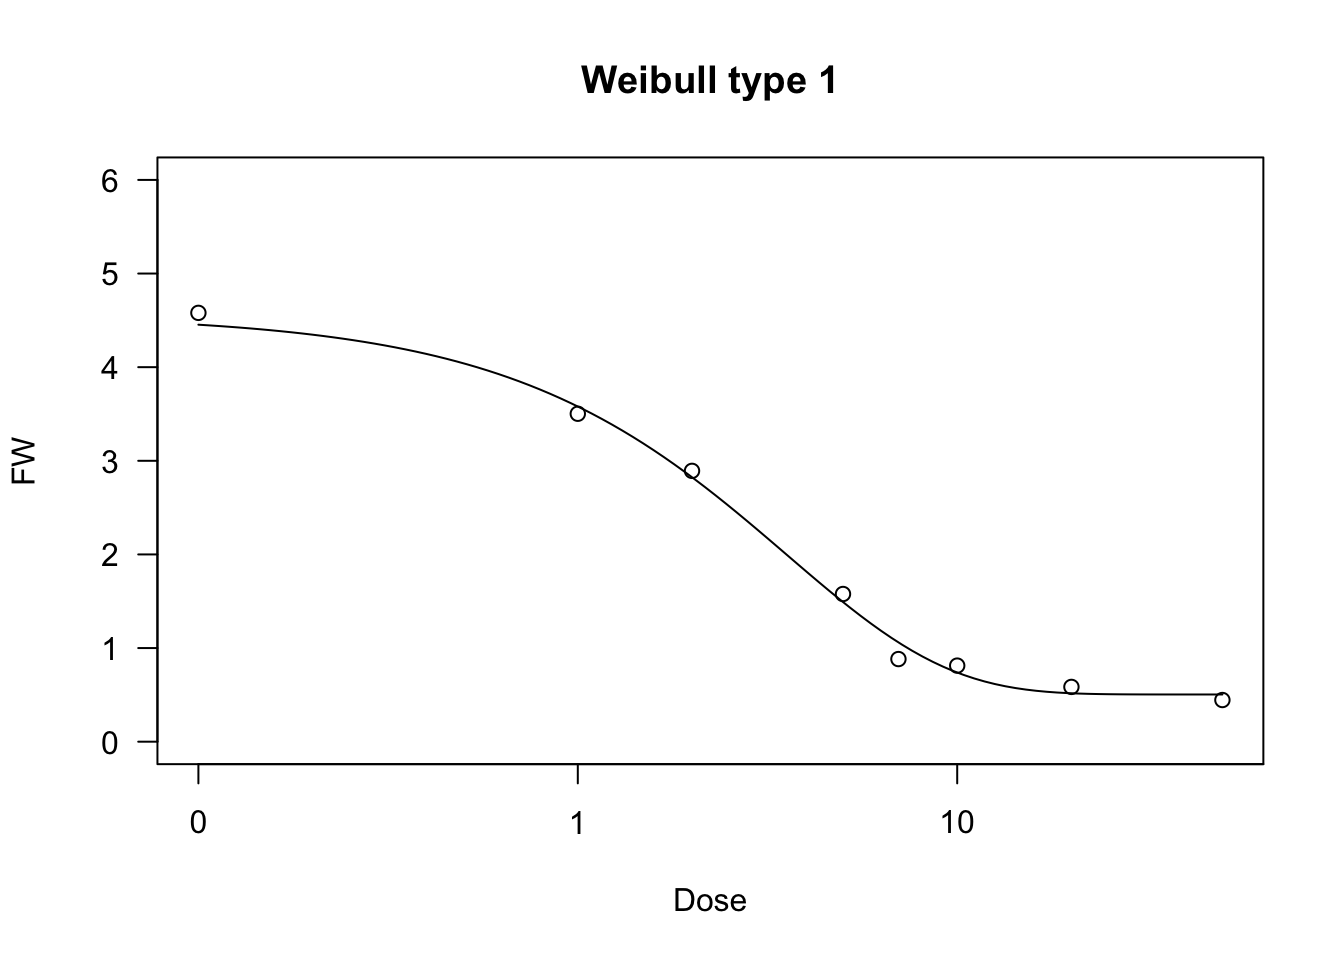
\includegraphics{_seedGerminationTutorial_files/figure-latex/unnamed-chunk-19-1.pdf}

\hypertarget{nonparametric-time-to-event-models}{%
\section{Nonparametric time-to-event models}\label{nonparametric-time-to-event-models}}

In some cases we are not willing to assume that the germination curve has a certain predefined shape, but we need an extra degree of flexibility. For example, emergences may proceed in successive flushes that are not easily described by using a sigmoidal curve. In these cases, we can fit a non-parametric model, whose shape is not pre-defined, but it is built by closely following the observed data. In survival analyses, time-to-event curves for interval censored data are estimated by using Nonparametric Maximum Likelihood Estimators (NPMLE), that are potentially interesting also for plant science.

For example, we can consider another factitious dataset, where the germination took place in two distinct flushes; a non-parametric maximum likelihood model can be fit by using the \texttt{NPMLE()} function, as shown in the box below.

\begin{Shaded}
\begin{Highlighting}[]
\NormalTok{dataset }\OtherTok{\textless{}{-}} \FunctionTok{read.csv}\NormalTok{(}\StringTok{"https://www.casaonofri.it/\_datasets/twoFlushes.csv"}\NormalTok{)}
\FunctionTok{head}\NormalTok{(dataset)}
\DocumentationTok{\#\#   timeBef timeAf nEmerg}
\DocumentationTok{\#\# 1       0      2      0}
\DocumentationTok{\#\# 2       2      4      1}
\DocumentationTok{\#\# 3       4      6     10}
\DocumentationTok{\#\# 4       6      8      9}
\DocumentationTok{\#\# 5       8     10      4}
\DocumentationTok{\#\# 6      10     12      0}
\NormalTok{te.npmle }\OtherTok{\textless{}{-}} \FunctionTok{drmte}\NormalTok{(nEmerg }\SpecialCharTok{\textasciitilde{}}\NormalTok{ timeBef }\SpecialCharTok{+}\NormalTok{ timeAf, }\AttributeTok{fct =} \FunctionTok{NPMLE}\NormalTok{(),}
                \AttributeTok{data =}\NormalTok{ dataset)}
\FunctionTok{summary}\NormalTok{(te.npmle)}
\DocumentationTok{\#\# }
\DocumentationTok{\#\# Model fitted: NPML estimator for time{-}to{-}event data}
\DocumentationTok{\#\# }
\DocumentationTok{\#\# Robust estimation: no }
\DocumentationTok{\#\# }
\DocumentationTok{\#\# Turnbull\textquotesingle{}s intervals and masses:}
\DocumentationTok{\#\# }
\DocumentationTok{\#\#            count   pdf   cdf Naive.SE}
\DocumentationTok{\#\# 1.(2,4]     1.00  0.02  0.02   0.0198}
\DocumentationTok{\#\# 1.(4,6]    10.00  0.20  0.22   0.0586}
\DocumentationTok{\#\# 1.(6,8]     9.00  0.18  0.40   0.0693}
\DocumentationTok{\#\# 1.(8,10]    4.00  0.08  0.48   0.0707}
\DocumentationTok{\#\# 1.(14,16]   1.00  0.02  0.50   0.0707}
\DocumentationTok{\#\# 1.(18,20]   1.00  0.02  0.52   0.0707}
\DocumentationTok{\#\# 1.(20,22]   1.00  0.02  0.54   0.0705}
\DocumentationTok{\#\# 1.(22,24]   4.00  0.08  0.62   0.0686}
\DocumentationTok{\#\# 1.(24,26]   7.00  0.14  0.76   0.0604}
\DocumentationTok{\#\# 1.(26,28]   6.00  0.12  0.88   0.0460}
\DocumentationTok{\#\# 1.(28,30]   3.00  0.06  0.94   0.0336}
\DocumentationTok{\#\# 1.(32,Inf)  3.00  0.06  1.00   0.0000}
\FunctionTok{par}\NormalTok{(}\AttributeTok{mfrow =} \FunctionTok{c}\NormalTok{(}\DecValTok{1}\NormalTok{,}\DecValTok{2}\NormalTok{))}

\FunctionTok{plot}\NormalTok{(te.npmle, }\AttributeTok{ylim =} \FunctionTok{c}\NormalTok{(}\DecValTok{0}\NormalTok{, }\DecValTok{1}\NormalTok{),}
     \AttributeTok{xlab =} \StringTok{"Time"}\NormalTok{, }\AttributeTok{ylab =} \StringTok{"Cumulative proportion of germinated seeds"}\NormalTok{,}
     \AttributeTok{main =} \StringTok{"Interpolation method"}\NormalTok{, }\AttributeTok{npmle.points =}\NormalTok{ T)}
\FunctionTok{plot}\NormalTok{(te.npmle, }\AttributeTok{ylim =} \FunctionTok{c}\NormalTok{(}\DecValTok{0}\NormalTok{, }\DecValTok{1}\NormalTok{),}
     \AttributeTok{xlab =} \StringTok{"Time"}\NormalTok{, }\AttributeTok{ylab =} \StringTok{"Cumulative proportion of germinated seeds"}\NormalTok{,}
     \AttributeTok{npmle.type =} \StringTok{"midpoint"}\NormalTok{, }\AttributeTok{shading =}\NormalTok{ F,}
     \AttributeTok{main =} \StringTok{"Midpoint imputation"}\NormalTok{)}
\end{Highlighting}
\end{Shaded}

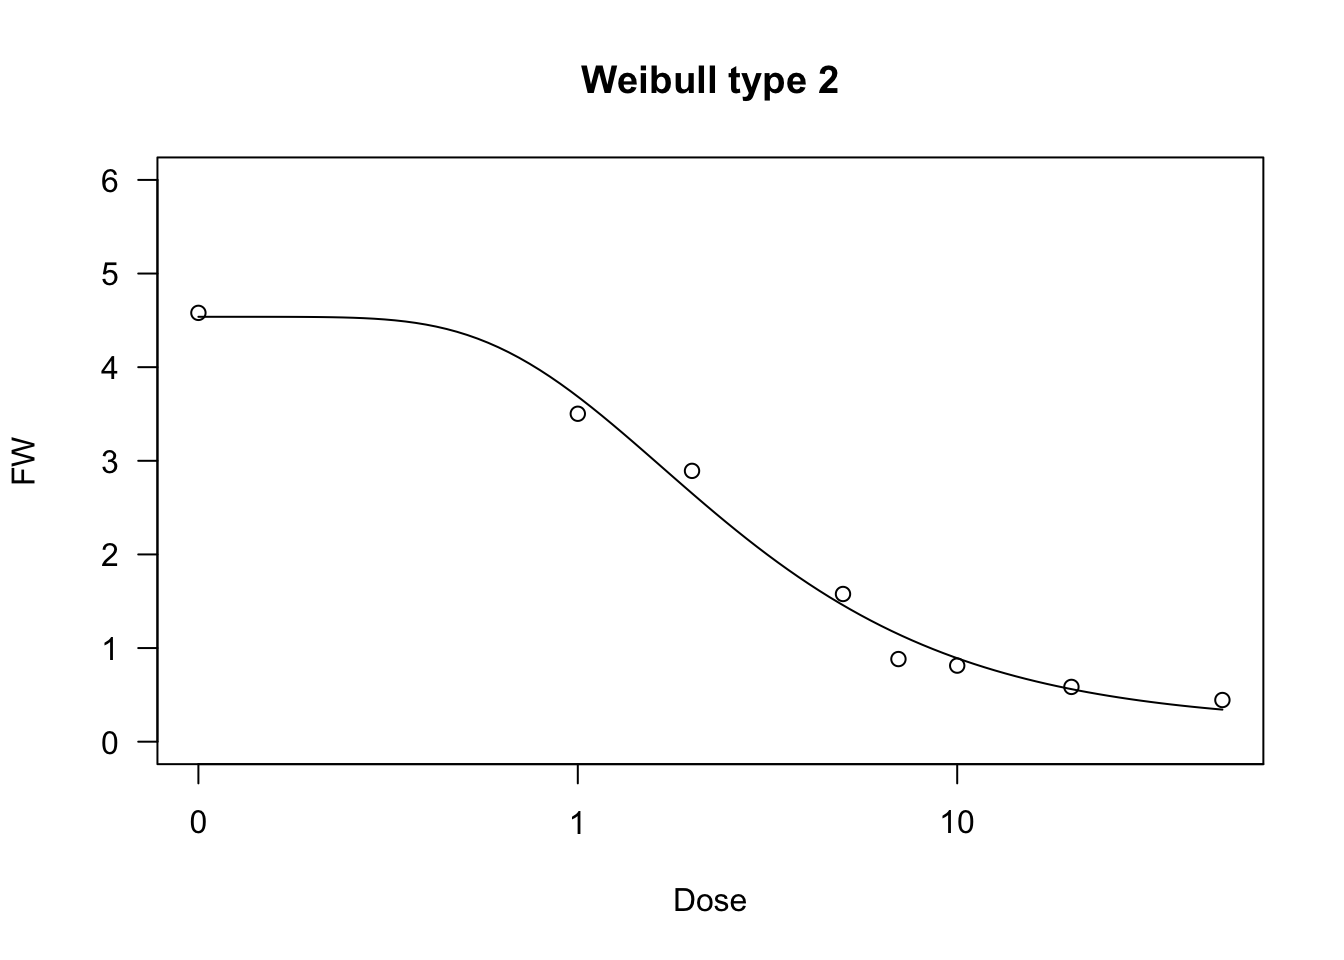
\includegraphics{_seedGerminationTutorial_files/figure-latex/unnamed-chunk-20-1.pdf}

With NPMLE, the time-to-event curve is only defined at the end of each time interval, while it is undefined elsewhere and it is (optionally) represented by a shaded area (Figure above, left). This shaded area reflects the uncertainty due to censoring.

Although we cannot know at what moment the nonparametric curve went up within the grey interval, we can make some reasonable assumptions. For example, we could assume that events are evenly spread within the interval, which is the approach taken in the `interval' package (Figure above, left panel). In the `survival' package and, most commonly, in survival analysis, it is assumed that the curve goes up in the middle of the interval (midpoint imputation; Figure above, right panel).

\hypertarget{kernel-density-estimators}{%
\section{Kernel density estimators}\label{kernel-density-estimators}}

NPMLEs are very flexible and they can be used to describe the progress to germination/emergence with, virtually, every type of datasets, also when the events took place in distinct flushes. However, we may be reluctant to accept a time-to-event curve with a stairstep shape, especially for prediction purposes. A further possibility to describe the time to event curve with a smooth and flexible model is to use a so-called Kernel Density Estimator (KDE). A KDE is built by considering the observed data, a Kernel function (usually gaussian) and a bandwith value, that controls the degree of smoothing; a nice post to see how Kernel density estimation works in practice can be found \href{https://mathisonian.github.io/kde/}{at this link here}.

In the box below we show that a KDE can be fitted to the observed data (same example as above) by using the \texttt{drmte()} function and setting the `fct' argument to \texttt{KDE()}. Please, note that this type of KDE is specifically modified to comply with censoring.

\begin{Shaded}
\begin{Highlighting}[]
\NormalTok{te.kde }\OtherTok{\textless{}{-}} \FunctionTok{drmte}\NormalTok{(nEmerg }\SpecialCharTok{\textasciitilde{}}\NormalTok{ timeBef }\SpecialCharTok{+}\NormalTok{ timeAf, }\AttributeTok{fct =} \FunctionTok{KDE}\NormalTok{(),}
                \AttributeTok{data =}\NormalTok{ dataset)}
\FunctionTok{summary}\NormalTok{(te.kde)}
\DocumentationTok{\#\# }
\DocumentationTok{\#\# Model fitted: Kernel estimator for the distribution function}
\DocumentationTok{\#\# }
\DocumentationTok{\#\# Robust estimation: no }
\DocumentationTok{\#\# }
\DocumentationTok{\#\# Bandwidth estimates:}
\DocumentationTok{\#\# }
\DocumentationTok{\#\#               Estimate}
\DocumentationTok{\#\# h:(bandwidth)   1.7871}
\FunctionTok{plot}\NormalTok{(te.kde, }\AttributeTok{ylim =} \FunctionTok{c}\NormalTok{(}\DecValTok{0}\NormalTok{, }\DecValTok{1}\NormalTok{),}
     \AttributeTok{xlab =} \StringTok{"Time"}\NormalTok{, }\AttributeTok{ylab =} \StringTok{"Cumulative proportion of germinated seeds"}\NormalTok{)}
\NormalTok{paf }\OtherTok{\textless{}{-}} \FunctionTok{KDE.fun}\NormalTok{(}\FunctionTok{seq}\NormalTok{(}\DecValTok{1}\NormalTok{,}\DecValTok{35}\NormalTok{, }\DecValTok{1}\NormalTok{), dataset}\SpecialCharTok{$}\NormalTok{timeBef, dataset}\SpecialCharTok{$}\NormalTok{timeAf, dataset}\SpecialCharTok{$}\NormalTok{nEmerg, }
               \AttributeTok{h =} \FloatTok{0.5}\NormalTok{)}
\FunctionTok{lines}\NormalTok{(paf }\SpecialCharTok{\textasciitilde{}} \FunctionTok{seq}\NormalTok{(}\DecValTok{1}\NormalTok{,}\DecValTok{35}\NormalTok{, }\DecValTok{1}\NormalTok{), }\AttributeTok{col =} \StringTok{"red"}\NormalTok{)}
\NormalTok{paf }\OtherTok{\textless{}{-}} \FunctionTok{KDE.fun}\NormalTok{(}\FunctionTok{seq}\NormalTok{(}\DecValTok{1}\NormalTok{,}\DecValTok{35}\NormalTok{, }\DecValTok{1}\NormalTok{), dataset}\SpecialCharTok{$}\NormalTok{timeBef, dataset}\SpecialCharTok{$}\NormalTok{timeAf, dataset}\SpecialCharTok{$}\NormalTok{nEmerg, }
               \AttributeTok{h =} \FloatTok{3.0}\NormalTok{)}
\FunctionTok{lines}\NormalTok{(paf }\SpecialCharTok{\textasciitilde{}} \FunctionTok{seq}\NormalTok{(}\DecValTok{1}\NormalTok{,}\DecValTok{35}\NormalTok{, }\DecValTok{1}\NormalTok{), }\AttributeTok{col =} \StringTok{"blue"}\NormalTok{)}
\end{Highlighting}
\end{Shaded}

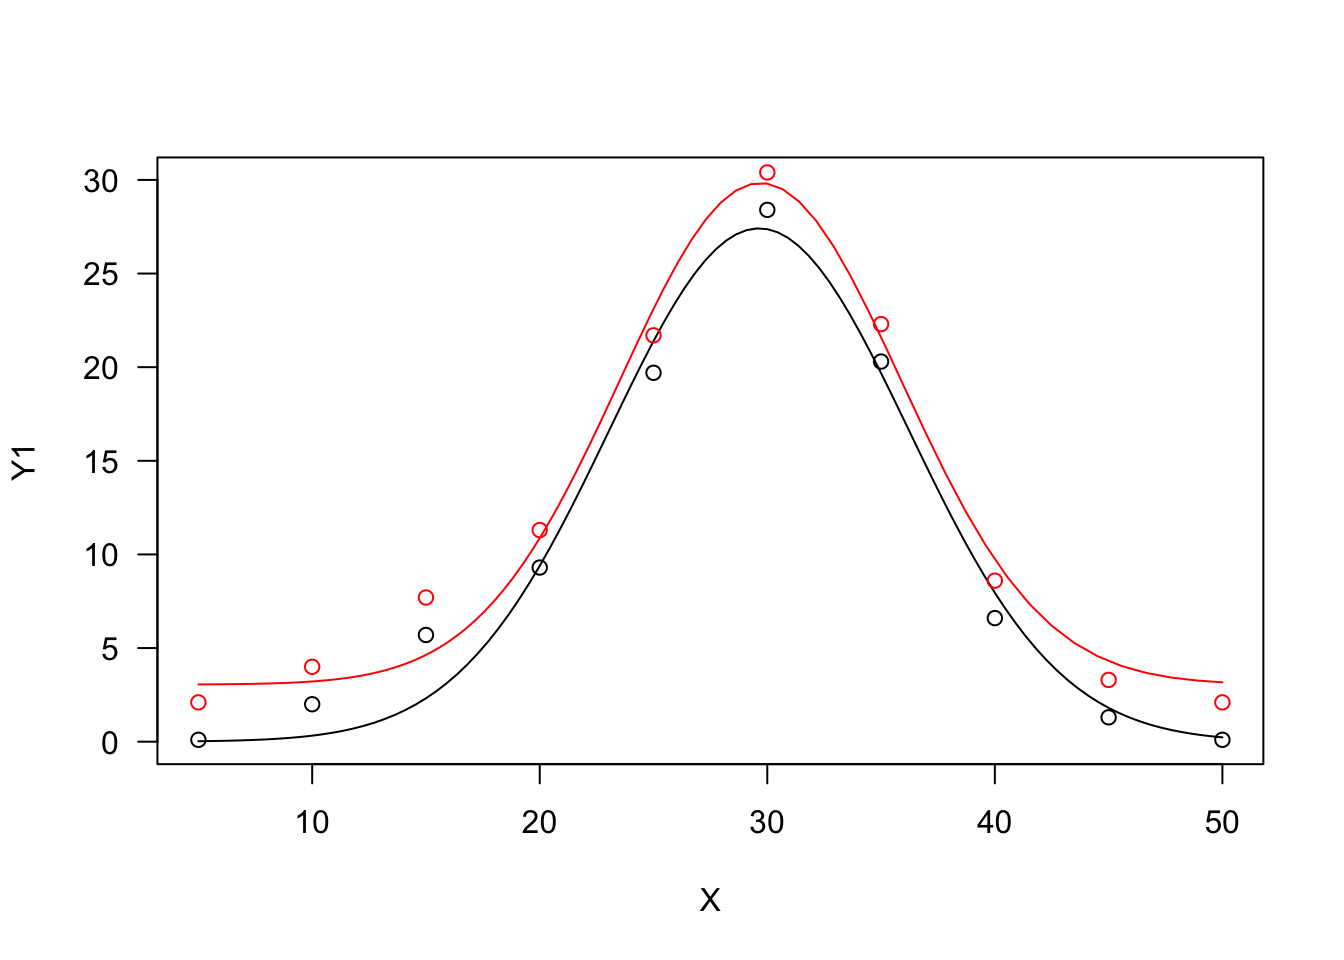
\includegraphics{_seedGerminationTutorial_files/figure-latex/unnamed-chunk-21-1.pdf}

We have augmented the above graph with three estimators: the blue one has a bandwidth \(h = 3\), the red one has \(b = 0.5\) and the black one has \(b = 1.7871\). Our aim was to show the effect of bandwidth selection on the resulting time-to-event curve, although it is usually necessary to apply an appropriate algorithm for the selection. The function \texttt{drmte()}, by default, uses the AMISE method and, unless you know what you are doing, we recommend that you stick to such an algorithm.

\hypertarget{ml-npmle-or-kde}{%
\section{ML, NPMLE or KDE?}\label{ml-npmle-or-kde}}

There is no rule to select the type of time-to-event model for seed germination/emergence and you will have to make your own choice and defend it at the publication stage. As a swift suggestion, I would say that a parametric model is to be preferred, unless it shows some visible signs of lack of fit.

Whatever model you select, fitting a time-to-event model may be the most unambiguous way to describe the progress to germination/emergence. In a future post, we will see that we can also compare time-to-event models for different experimental treatments and or environmental conditions, which is, most often, the central step in our process of data analyses, for seed germination/emergence assays.

\hypertarget{comparing-the-time-course-of-events-for-several-groups}{%
\chapter{Comparing the time course of events for several groups}\label{comparing-the-time-course-of-events-for-several-groups}}

Very often, seed scientists need to compare the germination behavior of different seed populations, e.g., different plant species, or one single plant species submitted to different temperatures, light conditions, priming treatments and so on. How should such a comparison be performed? For example, if we have submitted several seed samples to different environmental conditions, how do we decide whether the germinative response is affected by those environmental conditions?

If the case that we have replicates for all experimental treatments, e.g.~several Petri dishes, one possible line of attack is to take a summary measure for each dish and use that for further analyses, in a two-steps fashion. For example, we could take the total number of germinated seeds (Pmax) in each dish and use the resulting values to parameterise some sort of ANOVA-like model and test the significance of all effects.

This method of data analysis is known as `response feature analysis' and it may be regarded as `very traditional', in the sense that it is often found in literature; although it is not wrong, it is, undoubtedly, sub-optimal. Indeed, two seed lots submitted to different treatments may show the same total number of germinated seeds, but a different velocity or uniformity of germination. In other words, if we only consider, e.g., the Pmax, we can answer the question: ``do the seed lots differ for their germination capability?'', but not the more general question: ``are the seed lots different?''.

In order to answer this latter question, we should consider the entire time-course of germination and not only one single summary statistic. \textbf{In other words, we need a method to fit and compare several time-to-event curves.}

\hypertarget{a-motivating-example}{%
\section{A motivating example}\label{a-motivating-example}}

Let's take a practical approach and start from an example: a few years ago, some colleagues of mine studied the germination behavior of a plant species (\emph{Verbascum arcturus}), in different conditions. In detail, they considered the factorial combination of two storage periods (LONG and SHORT storage) and two temperature regimes (FIX: constant daily temperature of 20°C; ALT: alternating daily temperature regime, with 25°C during daytime and 15°C during night time, with a 12:12h photoperiod). If you are a seed scientist and are interested in this experiment, you'll find detail in Catara \emph{et al.} (2016).

If you are not a seed scientist, you may wonder why my colleagues made such an assay; well, there is evidence that, for some plant species, the germination ability improves over time, after seed maturation. Therefore, if we take seeds and store them for different periods of time, there might be an effect on their germination traits. Likewise, there is also evidence that germinations may be hindered if seed is not submitted to daily temperature fluctuations. For seed scientists, all these mechanisms are very important, as they permit to trigger the germinations when the environmental conditions are favorable for seedling survival.

Let's go back to our assay: the experimental design consisted of four experimental `combinations' (LONG-FIX, LONG-ALT, SHORT-FIX and SHORT-ALT) and four replicates for each combination. One replicate consisted of a Petri dish, that is a small plastic box containing humid blotting paper, with 25 seeds of \emph{V. arcturus}. In all, there were 16 Petri dishes, which were put in climatic chambers with the appropriate conditions. During the assay, my colleagues made daily inspections: germinated seeds were counted and removed from the dishes. Inspections were made for 15 days, until no more germinations could be observed.

The original dataset is available from a gitHub repository: let's load and have a look at it.

\begin{Shaded}
\begin{Highlighting}[]
\FunctionTok{rm}\NormalTok{(}\AttributeTok{list =} \FunctionTok{ls}\NormalTok{())}
\NormalTok{datasetOr }\OtherTok{\textless{}{-}} \FunctionTok{read.csv}\NormalTok{(}\StringTok{"https://raw.githubusercontent.com/OnofriAndreaPG/agroBioData/master/TempStorage.csv"}\NormalTok{, }\AttributeTok{header =}\NormalTok{ T, }\AttributeTok{check.names =}\NormalTok{ F)}
\FunctionTok{head}\NormalTok{(datasetOr)}
\DocumentationTok{\#\#   Dish Storage Temp 1 2 3 4 5 6 7 8 9 10 11 12 13 14 15}
\DocumentationTok{\#\# 1    1     Low  Fix 0 0 0 0 0 0 0 0 3  4  6  0  1  0  3}
\DocumentationTok{\#\# 2    2     Low  Fix 0 0 0 0 1 0 0 0 2  7  2  3  0  5  1}
\DocumentationTok{\#\# 3    3     Low  Fix 0 0 0 0 1 0 0 1 3  5  2  4  0  1  3}
\DocumentationTok{\#\# 4    4     Low  Fix 0 0 0 0 1 0 3 0 0  3  1  1  0  4  4}
\DocumentationTok{\#\# 5    5    High  Fix 0 0 0 0 0 0 0 0 1  2  5  4  2  3  0}
\DocumentationTok{\#\# 6    6    High  Fix 0 0 0 0 0 0 0 0 2  2  7  8  1  2  1}
\end{Highlighting}
\end{Shaded}

We have one row per Petri dish; the first three columns show, respectively, the dish number, storage and temperature conditions. The next 15 columns represent the inspection times (from 1 to 15) and contain the counts of germinated seeds. The research question is:

\emph{Is germination behavior affected by storage and temperature conditions?}

\hypertarget{fitting-several-time-to-event-curves}{%
\section{Fitting several time-to-event curves}\label{fitting-several-time-to-event-curves}}

The original dataset for our example is in a WIDE format and, as we have shown earlier in this tutorial, it is necessary to reshape it in LONG GROUPED format, by using the \texttt{melt\_te()} function in the `drcte' package.

The \texttt{melt\_te()} function needs to receive the columns storing the counts (`count\_cols = 4:18'), the columns storing the factor variables (`treat\_cols = c(``Dish'', ``Storage'', ``Temp'')'), a vector of monitoring times (`monitimes = 1:15') and a vector with the total number of seeds in each Petri dish (`n.subjects = rep(25,16)').

\begin{Shaded}
\begin{Highlighting}[]
\FunctionTok{library}\NormalTok{(drcte)}
\NormalTok{dataset }\OtherTok{\textless{}{-}} \FunctionTok{melt\_te}\NormalTok{(datasetOr, }\AttributeTok{count\_cols =} \DecValTok{4}\SpecialCharTok{:}\DecValTok{18}\NormalTok{, }
                   \AttributeTok{treat\_cols =} \FunctionTok{c}\NormalTok{(}\StringTok{"Dish"}\NormalTok{, }\StringTok{"Storage"}\NormalTok{, }\StringTok{"Temp"}\NormalTok{), }
                   \AttributeTok{monitimes =} \DecValTok{1}\SpecialCharTok{:}\DecValTok{15}\NormalTok{, }\AttributeTok{n.subjects =} \FunctionTok{rep}\NormalTok{(}\DecValTok{25}\NormalTok{, }\DecValTok{16}\NormalTok{))}
\FunctionTok{head}\NormalTok{(dataset, }\DecValTok{16}\NormalTok{)}
\DocumentationTok{\#\#    Dish Storage Temp Units timeBef timeAf count nCum propCum}
\DocumentationTok{\#\# 1     1     Low  Fix     1       0      1     0    0    0.00}
\DocumentationTok{\#\# 2     1     Low  Fix     1       1      2     0    0    0.00}
\DocumentationTok{\#\# 3     1     Low  Fix     1       2      3     0    0    0.00}
\DocumentationTok{\#\# 4     1     Low  Fix     1       3      4     0    0    0.00}
\DocumentationTok{\#\# 5     1     Low  Fix     1       4      5     0    0    0.00}
\DocumentationTok{\#\# 6     1     Low  Fix     1       5      6     0    0    0.00}
\DocumentationTok{\#\# 7     1     Low  Fix     1       6      7     0    0    0.00}
\DocumentationTok{\#\# 8     1     Low  Fix     1       7      8     0    0    0.00}
\DocumentationTok{\#\# 9     1     Low  Fix     1       8      9     3    3    0.12}
\DocumentationTok{\#\# 10    1     Low  Fix     1       9     10     4    7    0.28}
\DocumentationTok{\#\# 11    1     Low  Fix     1      10     11     6   13    0.52}
\DocumentationTok{\#\# 12    1     Low  Fix     1      11     12     0   13    0.52}
\DocumentationTok{\#\# 13    1     Low  Fix     1      12     13     1   14    0.56}
\DocumentationTok{\#\# 14    1     Low  Fix     1      13     14     0   14    0.56}
\DocumentationTok{\#\# 15    1     Low  Fix     1      14     15     3   17    0.68}
\DocumentationTok{\#\# 16    1     Low  Fix     1      15    Inf     8   NA      NA}
\end{Highlighting}
\end{Shaded}

In the resulting data frame, the column `timeAf' contains the time when the inspection was made and the column `count' contains the number of germinated seeds (e.g.~9 seeds were counted at day 9). These seeds did not germinate exactly at day 9; they germinated within the interval between two inspections, that is between day 8 and day 9. The beginning of the interval is given as the variable `timeBef'. Apart from these three columns, we have the columns for the blocking factor (`Dish' and `Units'; this latter column is added by the R function, but it is not useful in this case) and for the treatment factors (`Storage' and `Temp') plus two other additional columns (`nCum' and `propCum'), which we are not going to use for our analyses.

In this case, we have reasons to believe that the germination time-course can be described by using a parametric log-logistic time-to-event model, which can be estimated by using either the \texttt{drm()} function in the `drc' package (Ritz et al., 2019) or the \texttt{drmte()} function in the `drcte' package (Onofri et al., 2022). In both cases, we have to include the experimental factor (`curveid' argument), to specify that we want to fit a different curve for each combination of storage and temperature.

\begin{Shaded}
\begin{Highlighting}[]
\FunctionTok{library}\NormalTok{(tidyverse)}
\FunctionTok{library}\NormalTok{(drcte)}

\NormalTok{dataset }\OtherTok{\textless{}{-}}\NormalTok{ dataset }\SpecialCharTok{\%\textgreater{}\%} 
  \FunctionTok{mutate}\NormalTok{(}\FunctionTok{across}\NormalTok{(}\DecValTok{1}\SpecialCharTok{:}\DecValTok{3}\NormalTok{, }\AttributeTok{.fns =}\NormalTok{ factor))}
\NormalTok{mod1 }\OtherTok{\textless{}{-}} \FunctionTok{drmte}\NormalTok{(count }\SpecialCharTok{\textasciitilde{}}\NormalTok{ timeBef }\SpecialCharTok{+}\NormalTok{ timeAf, }\AttributeTok{fct =} \FunctionTok{loglogistic}\NormalTok{(),}
            \AttributeTok{data =}\NormalTok{ dataset, }
            \AttributeTok{curveid =}\NormalTok{ Temp}\SpecialCharTok{:}\NormalTok{Storage)}
\FunctionTok{summary}\NormalTok{(mod1)}
\DocumentationTok{\#\# }
\DocumentationTok{\#\# Model fitted: Log{-}logistic distribution of event times}
\DocumentationTok{\#\# }
\DocumentationTok{\#\# Robust estimation: no }
\DocumentationTok{\#\# }
\DocumentationTok{\#\# Parameter estimates:}
\DocumentationTok{\#\# }
\DocumentationTok{\#\#             Estimate Std. Error t{-}value   p{-}value    }
\DocumentationTok{\#\# b:Fix:Low   4.974317   0.819632  6.0690 1.287e{-}09 ***}
\DocumentationTok{\#\# b:Fix:High 11.476618   1.254439  9.1488 \textless{} 2.2e{-}16 ***}
\DocumentationTok{\#\# b:Alt:Low   7.854558   5.239825  1.4990    0.1339    }
\DocumentationTok{\#\# b:Alt:High 10.600439   1.014061 10.4534 \textless{} 2.2e{-}16 ***}
\DocumentationTok{\#\# d:Fix:Low   0.998474   0.150189  6.6481 2.968e{-}11 ***}
\DocumentationTok{\#\# d:Fix:High  0.861711   0.038987 22.1027 \textless{} 2.2e{-}16 ***}
\DocumentationTok{\#\# d:Alt:Low   1.405930   5.607576  0.2507    0.8020    }
\DocumentationTok{\#\# d:Alt:High  0.948113   0.024298 39.0208 \textless{} 2.2e{-}16 ***}
\DocumentationTok{\#\# e:Fix:Low  12.009974   0.987039 12.1677 \textless{} 2.2e{-}16 ***}
\DocumentationTok{\#\# e:Fix:High 10.906963   0.190532 57.2447 \textless{} 2.2e{-}16 ***}
\DocumentationTok{\#\# e:Alt:Low  17.014976  13.214513  1.2876    0.1979    }
\DocumentationTok{\#\# e:Alt:High  9.585255   0.166937 57.4183 \textless{} 2.2e{-}16 ***}
\DocumentationTok{\#\# {-}{-}{-}}
\DocumentationTok{\#\# Signif. codes:  0 \textquotesingle{}***\textquotesingle{} 0.001 \textquotesingle{}**\textquotesingle{} 0.01 \textquotesingle{}*\textquotesingle{} 0.05 \textquotesingle{}.\textquotesingle{} 0.1 \textquotesingle{} \textquotesingle{} 1}
\end{Highlighting}
\end{Shaded}

In a previous post I have described a log-logistic time-to-event model (\href{https://www.statforbiology.com/2021/stat_drcte_4-time-to-eventcurves/}{see here}), which has a sygmoidal shape, with the three parameters \(b\), \(d\) and \(e\). These parameters represent, respectively, the slope at inflection point, the higher asymptote (i.e.~the maximum proportion of germinated seeds) and the median germination time. As we have four curves, we have a number of 12 estimated parameters.

We see that the optimization routines returns an unreasonable value for the higher asymptote for one of the curves (\(d\) = 1.40 with Alt:Low); it is unreasonable because the maximum proportion of germinated seeds may not exceed 1. Therefore, we should refit the model by adding a constraint (\(d \le 1\)) for all the four curves. We can do so by setting the `upperl' argument to 1 for the 5\textsuperscript{th} through 8\textsuperscript{th} estimands.

\begin{Shaded}
\begin{Highlighting}[]
\NormalTok{mod1 }\OtherTok{\textless{}{-}} \FunctionTok{drmte}\NormalTok{(count }\SpecialCharTok{\textasciitilde{}}\NormalTok{ timeBef }\SpecialCharTok{+}\NormalTok{ timeAf, }\AttributeTok{fct =} \FunctionTok{loglogistic}\NormalTok{(),}
            \AttributeTok{data =}\NormalTok{ dataset, }
            \AttributeTok{curveid =}\NormalTok{ Temp}\SpecialCharTok{:}\NormalTok{Storage,}
            \AttributeTok{upperl =} \FunctionTok{c}\NormalTok{(}\ConstantTok{NA}\NormalTok{, }\ConstantTok{NA}\NormalTok{, }\ConstantTok{NA}\NormalTok{, }\ConstantTok{NA}\NormalTok{, }\DecValTok{1}\NormalTok{, }\DecValTok{1}\NormalTok{, }\DecValTok{1}\NormalTok{, }\DecValTok{1}\NormalTok{, }\ConstantTok{NA}\NormalTok{, }\ConstantTok{NA}\NormalTok{, }\ConstantTok{NA}\NormalTok{, }\ConstantTok{NA}\NormalTok{))}
\FunctionTok{summary}\NormalTok{(mod1)}
\DocumentationTok{\#\# }
\DocumentationTok{\#\# Model fitted: Log{-}logistic distribution of event times}
\DocumentationTok{\#\# }
\DocumentationTok{\#\# Robust estimation: no }
\DocumentationTok{\#\# }
\DocumentationTok{\#\# Parameter estimates:}
\DocumentationTok{\#\# }
\DocumentationTok{\#\#             Estimate Std. Error t{-}value   p{-}value    }
\DocumentationTok{\#\# b:Fix:Low   4.979665   0.818414  6.0845 1.168e{-}09 ***}
\DocumentationTok{\#\# b:Fix:High 11.471625   1.254025  9.1478 \textless{} 2.2e{-}16 ***}
\DocumentationTok{\#\# b:Alt:Low   8.408186   2.232712  3.7659 0.0001659 ***}
\DocumentationTok{\#\# b:Alt:High 10.605807   1.014523 10.4540 \textless{} 2.2e{-}16 ***}
\DocumentationTok{\#\# d:Fix:Low   0.997284   0.149235  6.6826 2.347e{-}11 ***}
\DocumentationTok{\#\# d:Fix:High  0.861709   0.038999 22.0955 \textless{} 2.2e{-}16 ***}
\DocumentationTok{\#\# d:Alt:Low   1.000000   0.881644  1.1342 0.2566920    }
\DocumentationTok{\#\# d:Alt:High  0.948132   0.024282 39.0468 \textless{} 2.2e{-}16 ***}
\DocumentationTok{\#\# e:Fix:Low  12.004534   0.981279 12.2336 \textless{} 2.2e{-}16 ***}
\DocumentationTok{\#\# e:Fix:High 10.907108   0.190613 57.2213 \textless{} 2.2e{-}16 ***}
\DocumentationTok{\#\# e:Alt:Low  15.903079   2.872327  5.5367 3.083e{-}08 ***}
\DocumentationTok{\#\# e:Alt:High  9.585297   0.166873 57.4406 \textless{} 2.2e{-}16 ***}
\DocumentationTok{\#\# {-}{-}{-}}
\DocumentationTok{\#\# Signif. codes:  0 \textquotesingle{}***\textquotesingle{} 0.001 \textquotesingle{}**\textquotesingle{} 0.01 \textquotesingle{}*\textquotesingle{} 0.05 \textquotesingle{}.\textquotesingle{} 0.1 \textquotesingle{} \textquotesingle{} 1}
\FunctionTok{plot}\NormalTok{(mod1, }\AttributeTok{log =} \StringTok{""}\NormalTok{, }\AttributeTok{legendPos =} \FunctionTok{c}\NormalTok{(}\DecValTok{6}\NormalTok{, }\DecValTok{1}\NormalTok{))}
\end{Highlighting}
\end{Shaded}

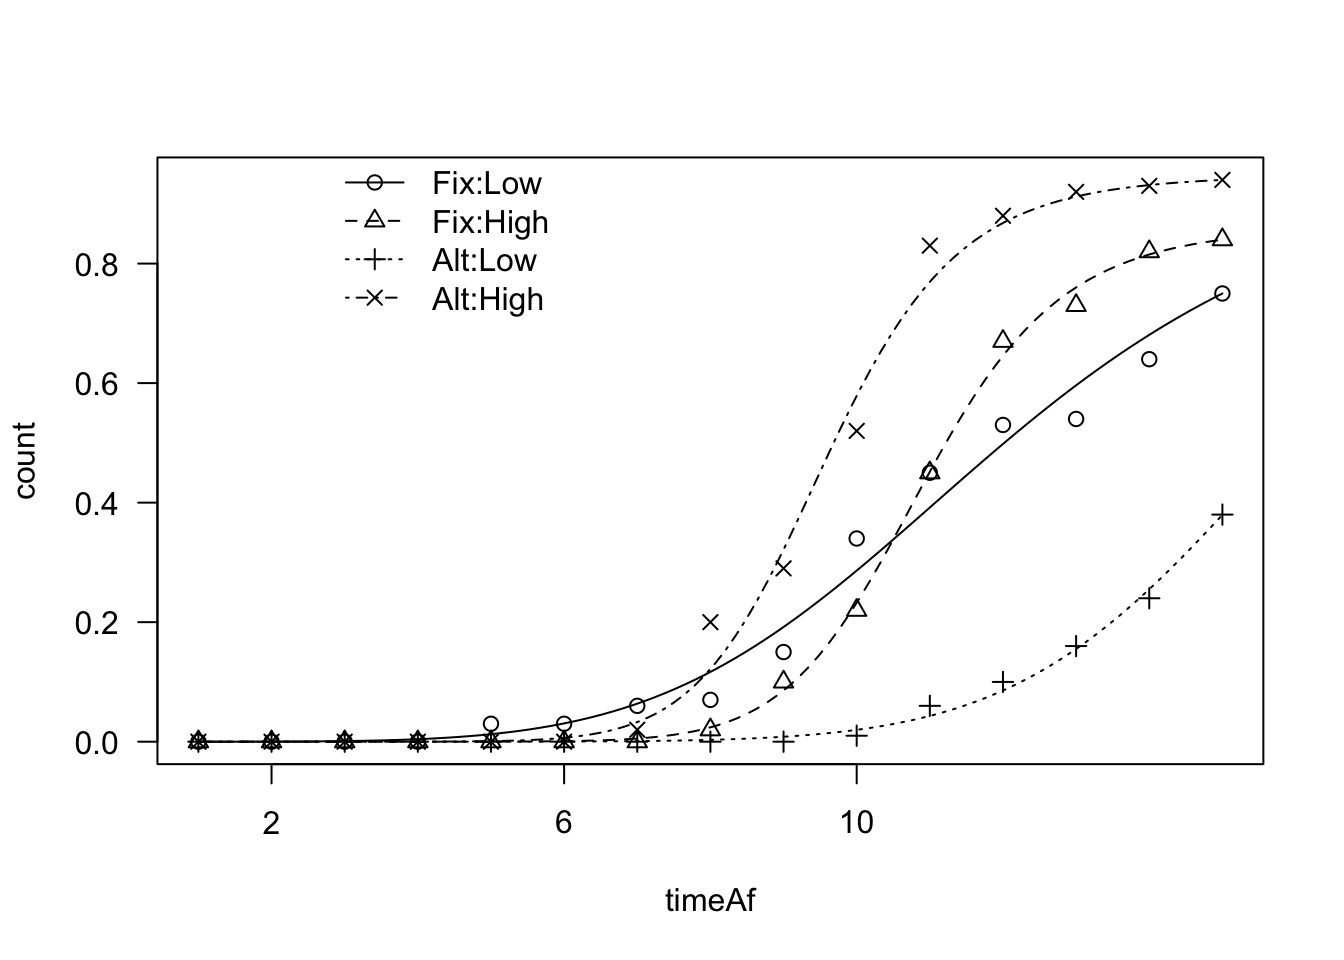
\includegraphics{_seedGerminationTutorial_files/figure-latex/unnamed-chunk-25-1.pdf}

From the graph we see that there are visible differences between the fitted curves (the legend considers the curves in alphabetical order, i.e.~1: Fix-Low, 2: Fix-High, 3: Alt-Low and 4: Alt-High). Now, the question is: could we say that those differences are only due to chance (null hypothesis)?

In order to make such a test, we could compare the logarithm of the likelihood for the fitted model with the logarithm of the likelihood for a `reduced' model, where all curves have been pooled into one common curve for all treatment levels. The higher the log-likelihood difference, the lowest the probability that the null is true (Likelihood Ratio Test; LRT).

A LRT for parametric models can be done with the \texttt{compCDF()} function in the `drcte' package, as shown in the box below.

\begin{Shaded}
\begin{Highlighting}[]
\FunctionTok{compCDF}\NormalTok{(mod1)}
\DocumentationTok{\#\# }
\DocumentationTok{\#\# }
\DocumentationTok{\#\# Likelihood ratio test}
\DocumentationTok{\#\# NULL: time{-}to{-}event curves are equal}
\DocumentationTok{\#\# }
\DocumentationTok{\#\# Observed LR value:  202.8052}
\DocumentationTok{\#\# Degrees of freedom:  9}
\DocumentationTok{\#\# P{-}value:  8.551556e{-}39}
\end{Highlighting}
\end{Shaded}

We see that the LR value, that relates to the difference between the two log-likelihoods, is rather high and equal to 202; when the null is true, this LR value has an approximate Chi-square distribution; accordingly, we see that the P-level is very low and, thus, the null should be rejected.

It general, the results of LRTs should be taken with care, particularly when the observed data are not independent from one another. Unfortunately, the lack of independence is an intrinsic characteristic of germination/emergence assays, where seeds are, most often, clustered within Petri dishes or other types of containers.

In this example, we got a very low p-level, which leaves us rather confident that the difference between time-to-event curves is significant. More generally, instead of relying on a chi-square approximation, we should better use a grouped-permutation approach. This technique is based on the idea that, when the difference between curves is not significant, we should be able to freely permute the labels (treatment level) among Petri dishes (clustering units) and, consequently, build an empirical distribution for the LR statistic under the null (permutation distribution). The p-level is related to the proportion of LR values in the permutation distribution that are higher than the observed value (i.e.: 202.8)

In the code below, we show how we can do this. The code is rather slow and, therefore, we should not use a very high number of permutation; the default is 199, that gives us a minimum p-value of 0.005. We see that we can confirm that the difference between curves is highly significant.

\begin{Shaded}
\begin{Highlighting}[]
\FunctionTok{compCDF}\NormalTok{(mod1, }\AttributeTok{type =} \StringTok{"permutation"}\NormalTok{, }\AttributeTok{units =}\NormalTok{ dataset}\SpecialCharTok{$}\NormalTok{Dishes)}
\DocumentationTok{\#\# Likelihood ratio test (permutation based)}
\DocumentationTok{\#\# NULL: time{-}to{-}event curves are equal}
\DocumentationTok{\#\# }
\DocumentationTok{\#\# Observed LR value:  202.8052}
\DocumentationTok{\#\# Degrees of freedom:  9}
\DocumentationTok{\#\# Naive P{-}value:  8.551556e{-}39}
\DocumentationTok{\#\# Permutation P{-}value (B = 199): 0.005}
\end{Highlighting}
\end{Shaded}

\hypertarget{comparing-non-parametric-curves}{%
\section{Comparing non-parametric curves}\label{comparing-non-parametric-curves}}

In the above example, we have decided to fit a parametric time-to-event model. However, in other situations, we might be interested in fitting a non-parametric time-to-event model (NPMLE; \href{https://www.statforbiology.com/2021/stat_drcte_4-time-to-eventcurves/}{see here}) and compare the curves for different treatment levels. In practice, nothing changes with respect to the approach I have shown above: first of all, we fit the NPMLEs with the following code:

\begin{Shaded}
\begin{Highlighting}[]
\NormalTok{modNP }\OtherTok{\textless{}{-}} \FunctionTok{drmte}\NormalTok{(count }\SpecialCharTok{\textasciitilde{}}\NormalTok{ timeBef }\SpecialCharTok{+}\NormalTok{ timeAf, }\AttributeTok{fct =} \FunctionTok{NPMLE}\NormalTok{(),}
            \AttributeTok{data =}\NormalTok{ dataset, }
            \AttributeTok{curveid =}\NormalTok{ Temp}\SpecialCharTok{:}\NormalTok{Storage)}
\FunctionTok{plot}\NormalTok{(modNP, }\AttributeTok{log =} \StringTok{""}\NormalTok{, }\AttributeTok{legendPos =} \FunctionTok{c}\NormalTok{(}\DecValTok{6}\NormalTok{, }\DecValTok{1}\NormalTok{))}
\end{Highlighting}
\end{Shaded}

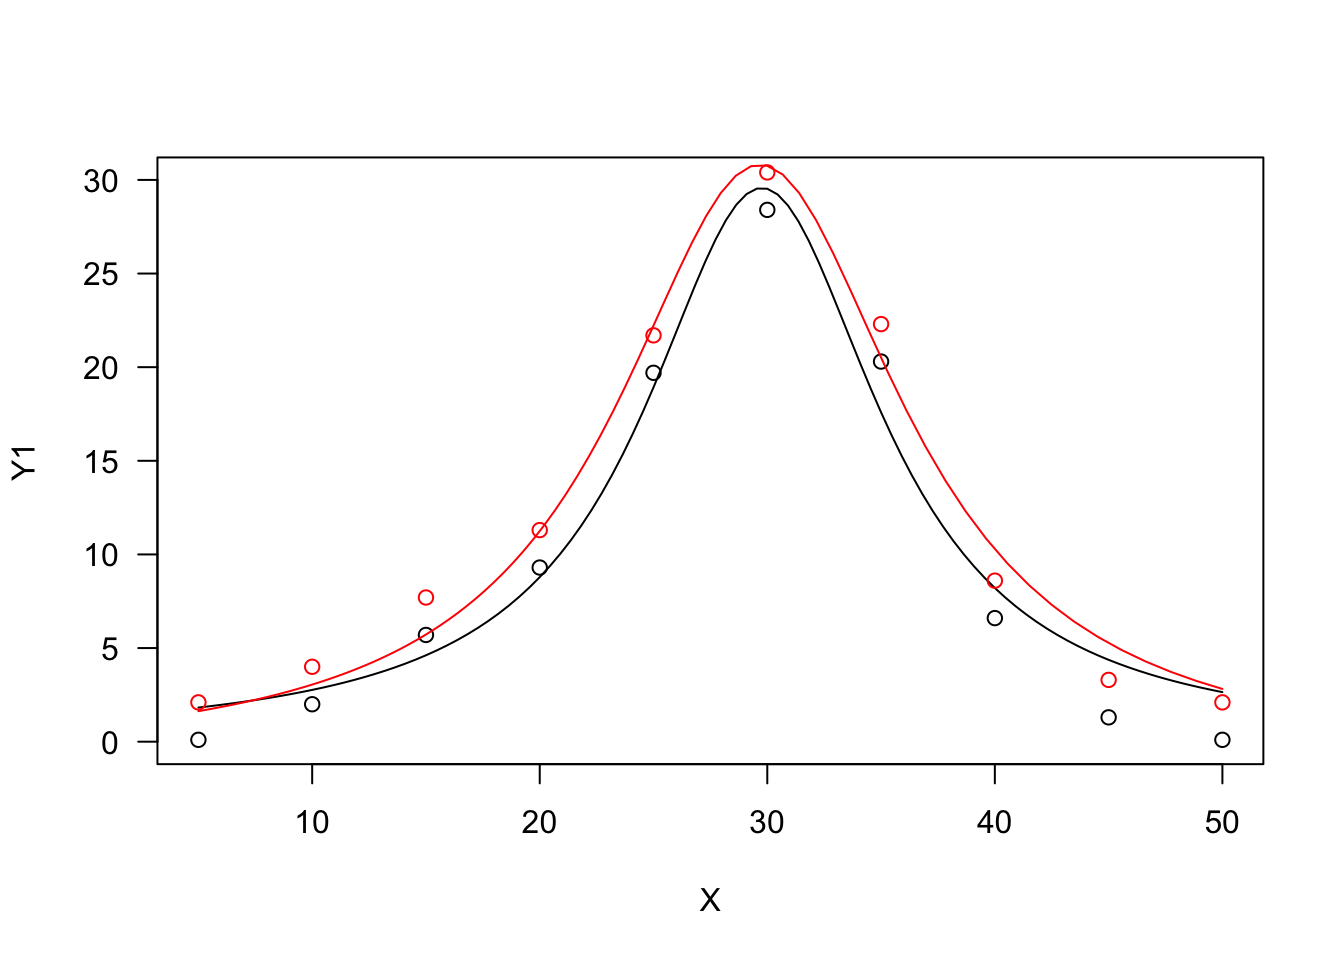
\includegraphics{_seedGerminationTutorial_files/figure-latex/unnamed-chunk-28-1.pdf}

Next, we compare the non-parametric curves, in the very same fashion as above:

\begin{Shaded}
\begin{Highlighting}[]
\FunctionTok{compCDF}\NormalTok{(modNP, }\AttributeTok{units =}\NormalTok{ dataset}\SpecialCharTok{$}\NormalTok{Units)}
\DocumentationTok{\#\# Exact Wilcoxon test (permutation form)}
\DocumentationTok{\#\# NULL: time{-}to{-}event curves are equal}
\DocumentationTok{\#\# }
\DocumentationTok{\#\#      level   n   Scores}
\DocumentationTok{\#\# 1  Fix:Low 100   2.5350}
\DocumentationTok{\#\# 2 Fix:High 100   6.4600}
\DocumentationTok{\#\# 3  Alt:Low 100 {-}51.2275}
\DocumentationTok{\#\# 4 Alt:High 100  42.2325}
\DocumentationTok{\#\# }
\DocumentationTok{\#\# Observed T value:  44.56}
\DocumentationTok{\#\# Permutation P{-}value (B = 199): 0.005}
\end{Highlighting}
\end{Shaded}

Obviously, with NPMLEs, a different test statistic is used in the background; the default one is the Wilcoxon rank sum score, although two types of log-rank scores are also implemented (Sun's scores and Finkelstein's scores; see Fay and Shaw 2010). Permutation based P-values are calculated and reported.

The approach is exactly the same with Kernel Density Estimators (KDE; \href{https://www.statforbiology.com/2021/stat_drcte_4-time-to-eventcurves/}{see here}). First we fit the four curves curves, by including the experimental factor as the `curveid' argument:

\begin{Shaded}
\begin{Highlighting}[]
\NormalTok{modKD }\OtherTok{\textless{}{-}} \FunctionTok{drmte}\NormalTok{(count }\SpecialCharTok{\textasciitilde{}}\NormalTok{ timeBef }\SpecialCharTok{+}\NormalTok{ timeAf, }\AttributeTok{fct =} \FunctionTok{KDE}\NormalTok{(),}
            \AttributeTok{data =}\NormalTok{ dataset, }
            \AttributeTok{curveid =}\NormalTok{ Temp}\SpecialCharTok{:}\NormalTok{Storage)}
\FunctionTok{plot}\NormalTok{(modKD, }\AttributeTok{log =} \StringTok{""}\NormalTok{, }\AttributeTok{legendPos =} \FunctionTok{c}\NormalTok{(}\DecValTok{6}\NormalTok{, }\DecValTok{1}\NormalTok{))}
\end{Highlighting}
\end{Shaded}

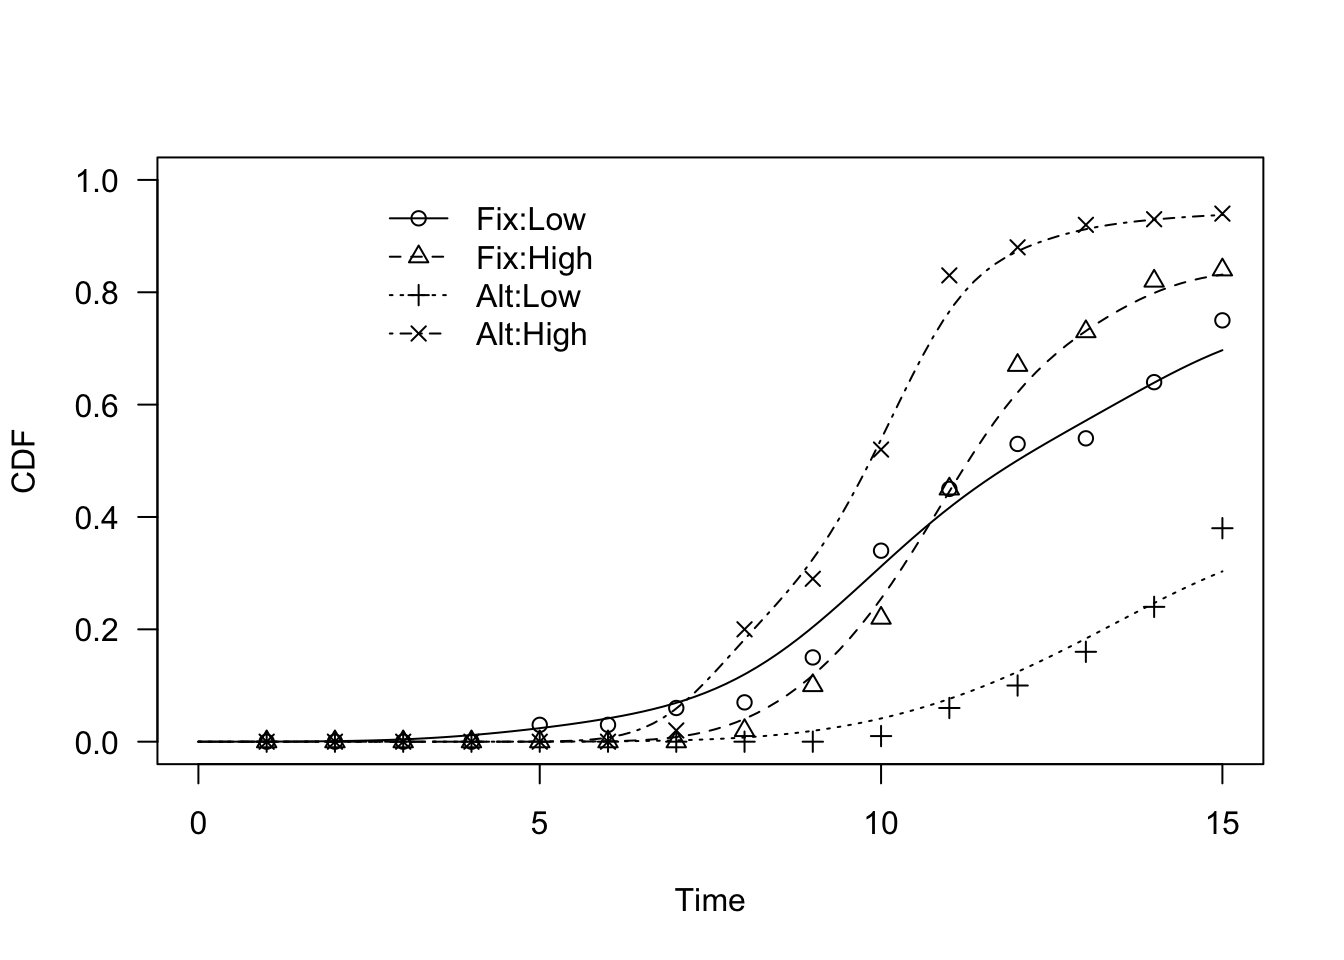
\includegraphics{_seedGerminationTutorial_files/figure-latex/unnamed-chunk-30-1.pdf}

Second, we compare those curves, by using the \texttt{compCDF()} function:

\begin{Shaded}
\begin{Highlighting}[]
\FunctionTok{compCDF}\NormalTok{(modKD, }\AttributeTok{units =}\NormalTok{ dataset}\SpecialCharTok{$}\NormalTok{Units)}
\DocumentationTok{\#\# Permuting groups}
\DocumentationTok{\#\# 1\% 1\% 2\% 2\% 3\% 3\% 4\% 4\% 5\% 5\% 6\% 6\% 7\% 7\% 8\% 8\% 9\% 9\% 10\% 10\% 11\% 11\%}
\DocumentationTok{\#\# 12\% 12\% 13\% 13\% 14\% 14\% 15\% 15\% 16\% 16\% 17\% 17\% 18\% 18\% 19\% 19\% 20\%}
\DocumentationTok{\#\# 20\% 21\% 21\% 22\% 22\% 23\% 23\% 24\% 24\% 25\% 25\% 26\% 26\% 27\% 27\% 28\% 28\%}
\DocumentationTok{\#\# 29\% 29\% 30\% 30\% 31\% 31\% 32\% 32\% 33\% 33\% 34\% 34\% 35\% 35\% 36\% 36\% 37\%}
\DocumentationTok{\#\# 37\% 38\% 38\% 39\% 39\% 40\% 40\% 41\% 41\% 42\% 42\% 43\% 43\% 44\% 44\% 45\% 45\%}
\DocumentationTok{\#\# 46\% 46\% 47\% 47\% 48\% 48\% 49\% 49\% 50\% 50\% 51\% 51\% 52\% 52\% 53\% 53\% 54\%}
\DocumentationTok{\#\# 54\% 55\% 55\% 56\% 56\% 57\% 57\% 58\% 58\% 59\% 59\% 60\% 60\% 61\% 61\% 62\% 62\%}
\DocumentationTok{\#\# 63\% 63\% 64\% 64\% 65\% 65\% 66\% 66\% 67\% 67\% 68\% 68\% 69\% 69\% 70\% 70\% 71\%}
\DocumentationTok{\#\# 71\% 72\% 72\% 73\% 73\% 74\% 74\% 75\% 75\% 76\% 76\% 77\% 77\% 78\% 78\% 79\% 79\%}
\DocumentationTok{\#\# 80\% 80\% 81\% 81\% 82\% 82\% 83\% 83\% 84\% 84\% 85\% 85\% 86\% 86\% 87\% 87\% 88\%}
\DocumentationTok{\#\# 88\% 89\% 89\% 90\% 90\% 91\% 91\% 92\% 92\% 93\% 93\% 94\% 94\% 95\% 95\% 96\% 96\%}
\DocumentationTok{\#\# 97\% 97\% 98\% 98\% 99\% 99\% 100\%}
\DocumentationTok{\#\# Permutation test based on a Cramer{-}von{-}Mises type distance (Barreiro{-}Ures et al., 2019)}
\DocumentationTok{\#\# NULL HYPOTHESIS: time{-}to{-}event curves are equal}
\DocumentationTok{\#\# }
\DocumentationTok{\#\#      level   n         D}
\DocumentationTok{\#\# 1  Fix:Low 100 0.0579661}
\DocumentationTok{\#\# 2 Fix:High 100 0.1347005}
\DocumentationTok{\#\# 3  Alt:Low 100 4.1378209}
\DocumentationTok{\#\# 4 Alt:High 100 3.8581487}
\DocumentationTok{\#\# }
\DocumentationTok{\#\# Observed D value =  2.0472}
\DocumentationTok{\#\# P value =  0.005}
\end{Highlighting}
\end{Shaded}

In this case, a Cramér‐von Mises type distance among curves is used (Barreiro-Ures et al., 2019), which, roughly speaking, is based on the integrated distance between the KDEs for the different groups and the pooled KDE for all groups. Permutation based P-values are also calculated and reported.

\hypertarget{fitting-time-to-event-models-with-environmental-covariates}{%
\chapter{Fitting time-to-event models with environmental covariates}\label{fitting-time-to-event-models-with-environmental-covariates}}

We have seen that time-to-event curves (e.g., germination or emergence curves) can be used to describe the time course of germinations/emergences for a seed lot and we have also seen that the effects of experimental factors on seed germination can be accounted for by coding a different time-to-event curve for each factor level.

In some cases, we might be interested in considering environmental variables, that are, perhaps, the most important factors to trigger germination/emergence. For example, let's consider either humidity content in the substrate, or temperature, or oxygen availability; it is clear that these variables play a fundamental role in determining germination extent and velocity and, therefore, they are very much studied by seed scientists. In principle, germination assays with environmental variables are straightforward to set up: several Petri dishes are submitted to different environmental conditions and germinations are inspected over time. What is the best method to analyse the resulting data and retrieve some important parameters, such as threshold temperatures (base, optimal or ceiling temperature) or base water potential?

It is important to anticipate that most environmental variables can be expressed on a quantitative scale; obviously when we make an experiment we are forced into selecting a subset of all possible, e.g., temperatures, such as 15, 20, 30°C, but that does not mean that we are not interested to what happens at, e.g., 18 or 22°C. From this point of view, quantitative variables are very different from qualitative variables, such as the different plant species that we have compared in previous sections of this tutorial.

In this post we will see an example of how we can account for the effects of water content in the substrate and include it in our time-to-event models. Of course, the same approach can be followed also with other types of environmental variables and, more generally, quantitative variables.

\hypertarget{hydro-time-to-event-models}{%
\section{Hydro-time-to-event models}\label{hydro-time-to-event-models}}

Let's consider the following example: the germination of rapeseed (\emph{Brassica napus} L. var. \emph{oleifera}, cv. Excalibur) was tested at fourteen different water potential levels (0, -0.03, -0.15, -0.3, -0.4, -0.5, -0.6, -0.7, -0.8, -0.9, -1, -1.1, -1.2, -1.5 MPa), which were created by using a polyethylene glycol solution (PEG 6000). For each water potential level, three replicated Petri dishes with 50 seeds each were incubated at 20°C. Germinated seeds were counted every 2-3 days for 14 days and they were removed from the dishes after germination.

The dataset was published by Pace et al.~(2012) and it is available as \texttt{rape} in the \texttt{drcSeedGerm} package, which needs to be installed from github (see below). Furthermore, the package \texttt{drcte} is necessary to fit time-to-event models and it should also be installed from gitHub. The following code loads the necessary packages, loads the dataset \texttt{rape} and shows the first six lines.

\begin{Shaded}
\begin{Highlighting}[]
\CommentTok{\# library(devtools)}
\CommentTok{\# install\_github("OnofriAndreaPG/drcSeedGerm")}
\CommentTok{\# install\_github("OnofriAndreaPG/drcte")}
\FunctionTok{library}\NormalTok{(drcSeedGerm)}
\FunctionTok{library}\NormalTok{(drcte)}
\FunctionTok{library}\NormalTok{(ggplot2)}
\FunctionTok{data}\NormalTok{(rape)}
\FunctionTok{head}\NormalTok{(rape)}
\DocumentationTok{\#\#   Psi Dish timeBef timeAf nSeeds nCum propCum}
\DocumentationTok{\#\# 1   0    1       0      3     49   49    0.98}
\DocumentationTok{\#\# 2   0    1       3      4      0   49    0.98}
\DocumentationTok{\#\# 3   0    1       4      5      0   49    0.98}
\DocumentationTok{\#\# 4   0    1       5      7      0   49    0.98}
\DocumentationTok{\#\# 5   0    1       7     10      0   49    0.98}
\DocumentationTok{\#\# 6   0    1      10     14      0   49    0.98}
\end{Highlighting}
\end{Shaded}

In the above data.frame, `timeAf' represents the moment when germinated seeds were counted, while 'timeBef' represents the previous inspection time (or the beginning of the assay). The column 'nSeeds' is the number of seeds that germinated during the time interval between `timeBef' and `timeAf. The 'propCum' column contains the cumulative proportions of germinated seeds and it is not necessary for time-to-event model fitting, although we can use it for plotting purposes.

\begin{Shaded}
\begin{Highlighting}[]
\FunctionTok{ggplot}\NormalTok{(rape, }\FunctionTok{aes}\NormalTok{(timeAf, propCum)) }\SpecialCharTok{+}
  \FunctionTok{geom\_point}\NormalTok{() }\SpecialCharTok{+}
  \FunctionTok{facet\_wrap}\NormalTok{(}\SpecialCharTok{\textasciitilde{}}\NormalTok{Psi) }\SpecialCharTok{+}
  \FunctionTok{scale\_x\_continuous}\NormalTok{(}\AttributeTok{name =} \StringTok{"Time (d)"}\NormalTok{) }\SpecialCharTok{+}
  \FunctionTok{scale\_y\_continuous}\NormalTok{(}\AttributeTok{name =} \StringTok{"Cumulative proportion of germinated seeds"}\NormalTok{)}
\end{Highlighting}
\end{Shaded}

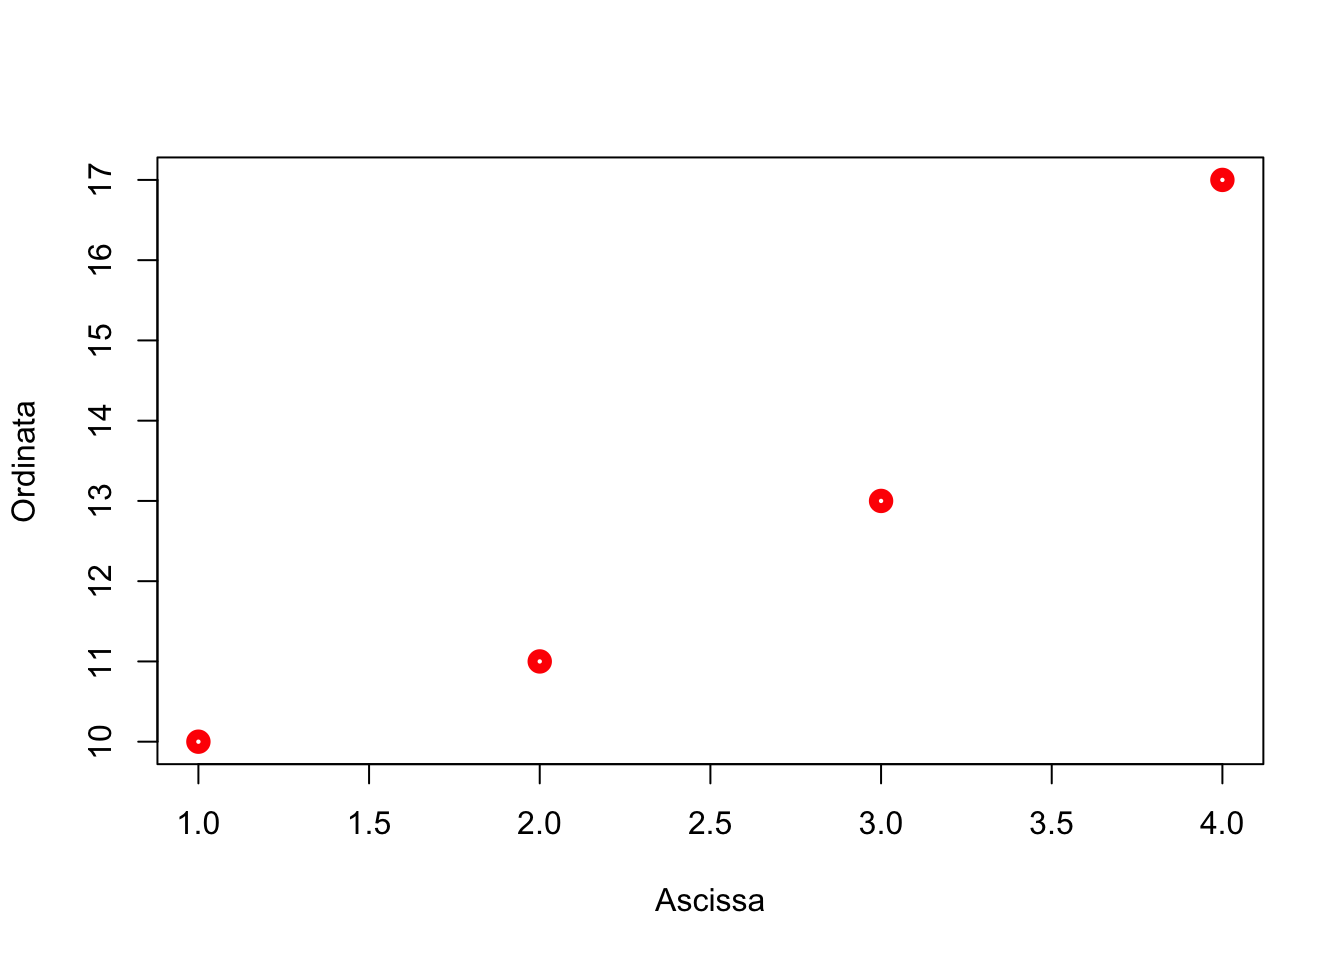
\includegraphics{_seedGerminationTutorial_files/figure-latex/unnamed-chunk-33-1.pdf}

The germination time-course is strongly affected by the water potential in the substrate, as this determines the ability of seeds to absorb water and, consequently, trigger the germination and emergence processes. Therefore, our obvious interest is to understand how the environmental factor affects the time-course of germination.

We have shown that a parametric time-to-event curve is defined as a cumulative probability function (\(\Phi\)), with three parameters:

\[P(t) = \Phi \left( b, d, e \right)\]
Considering \href{https://www.statforbiology.com/2021/stat_drcte_5-comparinglots/}{our previous post}, the most obvious extension of the above model is to allow for different \(b\), \(d\) and \(e\) value for each water potential level:

\[P(t, \Psi_i) = \Phi \left( b_i, d_i, e_i \right)\]

The first problem is that, for some water potential levels, germination did not occur and, for other levels, it occurred very quickly, so that no time-course of events could be observed (e.g., see the graph at 0 or -0.03 MPa). We say that we have `degenerated' time-to-event curves.

If we fit those curves by using the `curveid' argument, we are forced into fitting the same time-to-event model to all water potential levels (as shown in our previous post), and, therefore, the presence of degenerated curves provokes an error.

\begin{Shaded}
\begin{Highlighting}[]
\CommentTok{\# Not run}
\CommentTok{\# mod0 \textless{}{-} drmte(nSeeds \textasciitilde{} timeBef + timeAf, data = rape,}
\CommentTok{\#              curveid = Psi, fct = loglogistic())}
\end{Highlighting}
\end{Shaded}

This problem can be circumvented by using the \texttt{separate\ =\ TRUE} argument; in this case, the different curves are fitted independent of one another and we are not tied to fitting the same model for all water potential levels. Errors are raised when trying to fit parametric time-to-event models, but they do not stop the execution in R.

\begin{Shaded}
\begin{Highlighting}[]
\NormalTok{mod1 }\OtherTok{\textless{}{-}} \FunctionTok{drmte}\NormalTok{(nSeeds }\SpecialCharTok{\textasciitilde{}}\NormalTok{ timeBef }\SpecialCharTok{+}\NormalTok{ timeAf, }\AttributeTok{data =}\NormalTok{ rape,}
             \AttributeTok{curveid =}\NormalTok{ Psi, }\AttributeTok{fct =} \FunctionTok{loglogistic}\NormalTok{(),}
             \AttributeTok{separate =} \ConstantTok{TRUE}\NormalTok{)}
\DocumentationTok{\#\# Error in optim(startVec, opfct, hessian = TRUE, method = optMethod, control = list(maxit = maxIt,  : }
\DocumentationTok{\#\#   non{-}finite finite{-}difference value [3]}
\DocumentationTok{\#\# Error in optim(startVec, opfct, hessian = TRUE, method = optMethod, control = list(maxit = maxIt,  : }
\DocumentationTok{\#\#   non{-}finite value supplied by optim}
\DocumentationTok{\#\# Error in optim(startVec, opfct, hessian = TRUE, method = optMethod, control = list(maxit = maxIt,  : }
\DocumentationTok{\#\#   non{-}finite value supplied by optim}
\DocumentationTok{\#\# Error in optim(startVec, opfct, hessian = TRUE, method = optMethod, control = list(maxit = maxIt,  : }
\DocumentationTok{\#\#   non{-}finite value supplied by optim}
\FunctionTok{coef}\NormalTok{(mod1)}
\DocumentationTok{\#\#      d:{-}1.5      d:{-}1.2      d:{-}1.1        b:{-}1        d:{-}1 }
\DocumentationTok{\#\#  0.00000000  0.00000000  0.00000000 64.39202307  0.04666194 }
\DocumentationTok{\#\#        e:{-}1      b:{-}0.9      d:{-}0.9      e:{-}0.9      b:{-}0.8 }
\DocumentationTok{\#\#  8.36474946  5.83290900  0.55010281  5.87022056  3.73294999 }
\DocumentationTok{\#\#      d:{-}0.8      e:{-}0.8      b:{-}0.7      d:{-}0.7      e:{-}0.7 }
\DocumentationTok{\#\#  0.87889318  4.47105672  3.59940891  0.93592886  2.73025095 }
\DocumentationTok{\#\#      b:{-}0.6      d:{-}0.6      e:{-}0.6      b:{-}0.5      d:{-}0.5 }
\DocumentationTok{\#\#  1.46594380  1.00000000  0.73867461  1.09308015  0.96293123 }
\DocumentationTok{\#\#      e:{-}0.5      d:{-}0.4      d:{-}0.3     b:{-}0.15     d:{-}0.15 }
\DocumentationTok{\#\#  0.20862176  0.98444444  0.94333333  0.82546511  0.96143597 }
\DocumentationTok{\#\#     e:{-}0.15     d:{-}0.03         d:0 }
\DocumentationTok{\#\#  0.04345269  0.88666667  0.97333333}
\end{Highlighting}
\end{Shaded}

In particular, for the cases where a time-course of events cannot be estimated, the \texttt{drmte()} function resorts to fitting a simpler model, where only the \(d\) parameter is estimated (that is the maximum fraction of germinated seeds). In the box above, we can see the estimated parameters but no standard errors, which can be obtained by using the \texttt{summary()} method, although there are some statistical issues that we will consider in a following post.

\hypertarget{a-better-modelling-approach}{%
\section{A better modelling approach}\label{a-better-modelling-approach}}

The previous approach is clearly sub-optimal. First of all, the different water potential levels are assumed as independent, with no ordering and distances. In other words, we have a time-to-event curve for, e.g.~-0.9 MPa and -0.8 MPa, but we have no information about the time-to-event curve for any water potential levels in between. Furthermore, we have no estimates of some relevant hydro-time parameters, such as the \emph{base water potential}, that is fundamental to predict the germination/emergence in field conditions.

In order to account for the very nature of the water potential variable, we could code a time-to-event model where the three parameters are continuous functions of \(\Psi\):

\[P(t, \Psi) = \Phi \left( b(\Psi), d(\Psi), e(\Psi) \right)\]

We followed such an approach in a relatively recent publication (Onofri et al., 2018) and we also spoke about this in a \href{https://www.statforbiology.com/2020/stat_seedgermination_ht1step/}{recent post}. In detail, we considered a log-logistic cumulative distribution function:

\[P(t) = \frac{ d }{1 + \exp \left\{ b \left[ \log(t) - \log( e ) \right] \right\} }\]

where \(e\) is the median germination time, \(b\) is the slope at the inflection point and \(d\) is the maximum germinated proportion. Considering that the germination rate is the inverse of germination time, we replaced \(e = 1/GR_{50}\) and wrote the three parameters as functions of \(\Psi\):

\[P(t, \Psi) = \frac{ d(\Psi) }{1 + \exp \left\{ b(\Psi) \left[ \log(t) - \log(1 / \left[ GR_{50}(\Psi) \right] ) \right] \right\} }\]

where:

\[{\begin{array}{l}
GR_{50}(\Psi) = \textrm{max} \left( \frac{\Psi - \Psi_{b}}{\theta_H}; 0 \right)\\
d(\Psi ) = \textrm{max} \left\{ G \, \left[ 1 - \exp \left( \frac{ \Psi - \Psi_b }{\sigma_{\Psi_b}} \right) \right]; 0 \right\}\\
b(\Psi) = b
\end{array}}\]

The parameters are:

\begin{enumerate}
\def\labelenumi{\arabic{enumi}.}
\tightlist
\item
  \(\Psi_{b}\), that is the median base water potential in the seed lot (in \emph{MPa}),
\item
  \(\theta_H\), that is the hydro-time constant (in \emph{MPa day} or \emph{MPa hour})
\item
  \(\sigma_{\Psi_b}\), that represents the variability of \(\Psi_b\) within the population,
\item
  \(G\), that is the germinable fraction, accounting for the fact that \(d\) may not reach 1, regardless of time and water potential.
\item
  \(b\) (slope parameter) that is assumed to be constant and independent on \(\Psi\).
\end{enumerate}

In the end, our hydro-time model is composed by four sub-models:

\begin{enumerate}
\def\labelenumi{\arabic{enumi}.}
\tightlist
\item
  a cumulative probability function (log-logistic, in our example), based on the three parameters \(d\), \(b\) and \(e = 1/GR50\);
\item
  a sub-model expressing \(d\) as a function of \(\Psi\);
\item
  a sub-model expressing \(GR50\) as a function of \(\Psi\);
\item
  a sub-model expressing \(b\) as a function of \(\Psi\), although, this was indeed a simple identity model \(b(\Psi) = b\).
\end{enumerate}

This hydro-time-to-event model was implemented in R as the \texttt{HTE1()} function, and it is available within the \texttt{drcSeedGerm} package, together with the appropriate self-starting routine. It can be fitted by using the \texttt{drmte()} function in the \texttt{drcte} package and the \texttt{coef()} function can be used to retrieve the parameter estimates.

\begin{Shaded}
\begin{Highlighting}[]
\NormalTok{modHTE }\OtherTok{\textless{}{-}} \FunctionTok{drmte}\NormalTok{(nSeeds }\SpecialCharTok{\textasciitilde{}}\NormalTok{ timeBef }\SpecialCharTok{+}\NormalTok{ timeAf }\SpecialCharTok{+}\NormalTok{ Psi, }
                \AttributeTok{data =}\NormalTok{ rape, }\AttributeTok{fct =} \FunctionTok{HTE1}\NormalTok{())}
\FunctionTok{coef}\NormalTok{(modHTE)}
\DocumentationTok{\#\#         G:(Intercept)      Psib:(Intercept) sigmaPsib:(Intercept) }
\DocumentationTok{\#\#             0.9577918            {-}1.0397239             0.1108891 }
\DocumentationTok{\#\#    thetaH:(Intercept)         b:(Intercept) }
\DocumentationTok{\#\#             0.9061385             4.0273963}
\end{Highlighting}
\end{Shaded}

As we said before, we are also interested in standard errors for model parameters; we will address this issue in another post. It is important to note that this model gives us the ability of predicting germination at any water potential levels and it is not restrained to the values that we included in the experimental design. Furthermore, we have reliable estimates of \(\Psi_{b}\) and \(\theta_H\), which we can use for prediction purposes in field conditions.

\hypertarget{another-modelling-approach}{%
\section{Another modelling approach}\label{another-modelling-approach}}

Another type of hydro-time model was proposed by Bradford (2002) and later extended by Mesgaran et al., (2013). These authors, instead of modifying a traditional log-logistic distribution to include the environmental covariate, wrote a totally new cumulative distribution function, based on theoretical underpinnings relating to the distribution of base water potential within a seed population. Their model is:

\[ P(t, \Psi) = \Phi \left\{ \frac{\Psi - (\theta_H / t) -\Psi_b }{\sigma_{\Psi_b}} \right\}\]

where \(\Phi\) is a gaussian cumulative distribution function for base water potential. More information on how this model can be obtained from the original papers; it is, however, important to highlight that it is assumed that base water potential changes from seed to seeds within the population, according to a gaussian distribution function. The cumulative distribution function of event times is indirectly modelled, but it is not, in itself, gaussian (you see that \(t\) is at the denominator).

Mesgaran et al (2013) suggested that \(\Phi\) may not be gaussian and proposed several alternatives, so that, in all, we have six possible hydro-time-to-event models, which we have implemented within the \texttt{drcSeedGerm} package:

\begin{enumerate}
\def\labelenumi{\arabic{enumi}.}
\tightlist
\item
  gaussian (function \texttt{HTnorm()})
\item
  logistic (function \texttt{HTL()})
\item
  Gumbel (function \texttt{HTG()})
\item
  log-logistic (function \texttt{HTLL()})
\item
  Weibull (Type I) (function \texttt{HTW1()})
\item
  Weibull (Type II) (function \texttt{HTW2()})
\end{enumerate}

These equations are given at the end of this post. The code to fit those models is given below:

\begin{Shaded}
\begin{Highlighting}[]
\NormalTok{mod1 }\OtherTok{\textless{}{-}} \FunctionTok{drmte}\NormalTok{(nSeeds }\SpecialCharTok{\textasciitilde{}}\NormalTok{ timeBef }\SpecialCharTok{+}\NormalTok{ timeAf }\SpecialCharTok{+}\NormalTok{ Psi, }
              \AttributeTok{data =}\NormalTok{ rape, }\AttributeTok{fct =} \FunctionTok{HTnorm}\NormalTok{())}
\NormalTok{mod2 }\OtherTok{\textless{}{-}} \FunctionTok{drmte}\NormalTok{(nSeeds }\SpecialCharTok{\textasciitilde{}}\NormalTok{ timeBef }\SpecialCharTok{+}\NormalTok{ timeAf }\SpecialCharTok{+}\NormalTok{ Psi,}
              \AttributeTok{data =}\NormalTok{ rape, }\AttributeTok{fct =} \FunctionTok{HTL}\NormalTok{())}
\NormalTok{mod3 }\OtherTok{\textless{}{-}} \FunctionTok{drmte}\NormalTok{(nSeeds }\SpecialCharTok{\textasciitilde{}}\NormalTok{ timeBef }\SpecialCharTok{+}\NormalTok{ timeAf }\SpecialCharTok{+}\NormalTok{ Psi,}
              \AttributeTok{data =}\NormalTok{ rape, }\AttributeTok{fct =} \FunctionTok{HTG}\NormalTok{())}
\NormalTok{mod4 }\OtherTok{\textless{}{-}} \FunctionTok{drmte}\NormalTok{(nSeeds }\SpecialCharTok{\textasciitilde{}}\NormalTok{ timeBef }\SpecialCharTok{+}\NormalTok{ timeAf }\SpecialCharTok{+}\NormalTok{ Psi,}
            \AttributeTok{data =}\NormalTok{ rape, }\AttributeTok{fct =} \FunctionTok{HTLL}\NormalTok{())}
\NormalTok{mod5 }\OtherTok{\textless{}{-}} \FunctionTok{drmte}\NormalTok{(nSeeds }\SpecialCharTok{\textasciitilde{}}\NormalTok{ timeBef }\SpecialCharTok{+}\NormalTok{ timeAf }\SpecialCharTok{+}\NormalTok{ Psi,}
            \AttributeTok{data =}\NormalTok{ rape, }\AttributeTok{fct =} \FunctionTok{HTW1}\NormalTok{())}
\NormalTok{mod6 }\OtherTok{\textless{}{-}} \FunctionTok{drmte}\NormalTok{(nSeeds }\SpecialCharTok{\textasciitilde{}}\NormalTok{ timeBef }\SpecialCharTok{+}\NormalTok{ timeAf }\SpecialCharTok{+}\NormalTok{ Psi,}
            \AttributeTok{data =}\NormalTok{ rape, }\AttributeTok{fct =} \FunctionTok{HTW2}\NormalTok{())}
\end{Highlighting}
\end{Shaded}

What is the best model for this dataset? Let's use the Akaike's Information Criterion (AIC: the lowest, the best) to decide; we see that \texttt{modHTE} was the best fitting one, followed by \texttt{mod4}.

\begin{Shaded}
\begin{Highlighting}[]
\FunctionTok{AIC}\NormalTok{(mod1, mod2, mod3, mod4, mod5, mod6, modHTE)}
\DocumentationTok{\#\#         df      AIC}
\DocumentationTok{\#\# mod1   291 3516.914}
\DocumentationTok{\#\# mod2   291 3300.824}
\DocumentationTok{\#\# mod3   291 3097.775}
\DocumentationTok{\#\# mod4   290 2886.608}
\DocumentationTok{\#\# mod5   290 2889.306}
\DocumentationTok{\#\# mod6   290 3009.023}
\DocumentationTok{\#\# modHTE 289 2832.481}
\end{Highlighting}
\end{Shaded}

It is important not to neglect a graphical inspection of model fit. The \texttt{plot()} method does not work with time-to-event curves with additional covariates (apart from time). However, we can retrieve the fitted data by using the \texttt{plotData()} function and use those predictions within the \texttt{ggplot()} function. The box below shows the appropriate coding.

\begin{Shaded}
\begin{Highlighting}[]
\FunctionTok{library}\NormalTok{(ggplot2)}
\NormalTok{tab }\OtherTok{\textless{}{-}} \FunctionTok{plotData}\NormalTok{(modHTE)}

\FunctionTok{ggplot}\NormalTok{() }\SpecialCharTok{+}
  \FunctionTok{geom\_point}\NormalTok{(}\AttributeTok{data =}\NormalTok{ rape, }\AttributeTok{mapping =} \FunctionTok{aes}\NormalTok{(}\AttributeTok{x =}\NormalTok{ timeAf, }\AttributeTok{y =}\NormalTok{ propCum),}
            \AttributeTok{col =} \StringTok{"red"}\NormalTok{) }\SpecialCharTok{+}
  \FunctionTok{geom\_line}\NormalTok{(}\AttributeTok{data =}\NormalTok{ tab}\SpecialCharTok{$}\NormalTok{plotFits, }\AttributeTok{mapping =} \FunctionTok{aes}\NormalTok{(}\AttributeTok{x =}\NormalTok{ timeAf, }\AttributeTok{y =}\NormalTok{ CDF)) }\SpecialCharTok{+}
  \FunctionTok{facet\_wrap}\NormalTok{(}\SpecialCharTok{\textasciitilde{}}\NormalTok{ Psi) }\SpecialCharTok{+}
  \FunctionTok{scale\_x\_continuous}\NormalTok{(}\AttributeTok{name =} \StringTok{"Time (d)"}\NormalTok{) }\SpecialCharTok{+}
  \FunctionTok{scale\_y\_continuous}\NormalTok{(}\AttributeTok{name =} \StringTok{"Cumulative proportion of germinated seeds"}\NormalTok{)}
\DocumentationTok{\#\# Warning: Removed 42 rows containing missing values (\textasciigrave{}geom\_point()\textasciigrave{}).}
\end{Highlighting}
\end{Shaded}

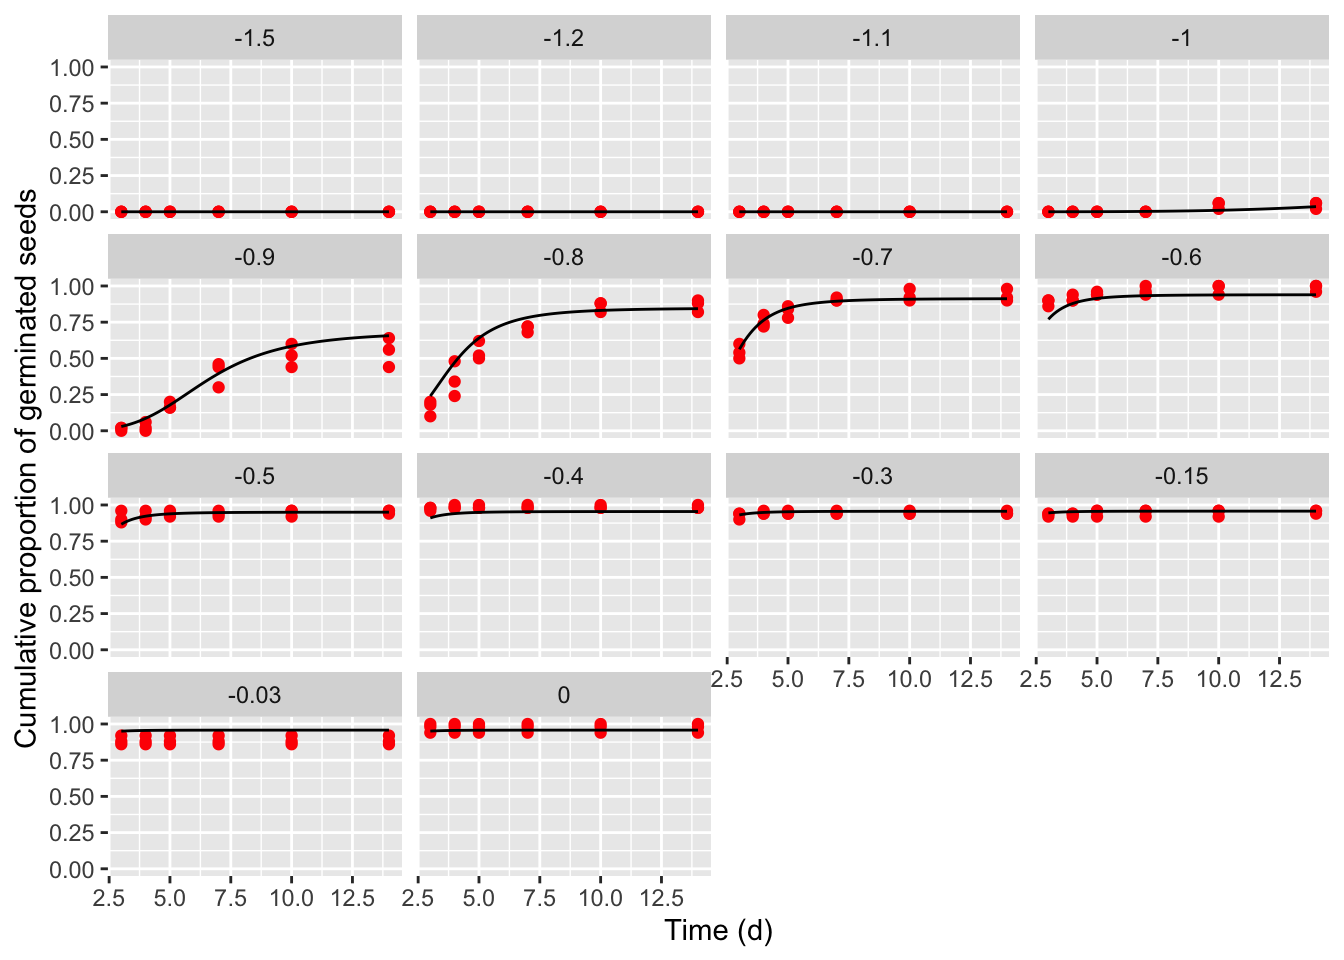
\includegraphics{_seedGerminationTutorial_files/figure-latex/unnamed-chunk-39-1.pdf}

\hypertarget{further-detail}{%
\section{Further detail}\label{further-detail}}

Let us conclude this section by giving some detail on all other models in Mesgaran et al (2913; slightly reparameterised). In same cases \(\Psi_b\) has been replaced by \(\mu\), that is the location parameter of the cumulative distribution function of base water potential, but it is not the median value. On the other hand, \(\delta\) is the shifting parameter for all logarithm based distributions; indeed, logarithm based distribution are only defined for strictly positive variables, while we know that water potential usually assumes negative values. The shifting parameters is used to shift the cumulative distribution function to the right, so that negative values are allowed.

\hypertarget{htl}{%
\subsection{\texorpdfstring{\texttt{HTL()}}{HTL()}}\label{htl}}

\[ G(t, \Psi) = \frac{1}{1 + exp \left[ - \frac{  \Psi  - \left( \theta _H/t \right) - \Psi_{b} } {\sigma}  \right] }\]

\hypertarget{htg}{%
\subsection{\texorpdfstring{\texttt{HTG()}}{HTG()}}\label{htg}}

\[ G(t, \Psi) = \exp \left\{ { - \exp \left[ { - \left( {\frac{{\Psi - (\theta _H / t ) - \mu }}{\sigma }} \right)} \right]} \right\} \]

\hypertarget{htll}{%
\subsection{\texorpdfstring{\texttt{HTLL()}}{HTLL()}}\label{htll}}

\[ G(t, \Psi) = \frac{1}{1 + \exp \left\{ \frac{ \log \left[ \Psi  - \left( \frac{\theta _H}{t} \right) + \delta \right] - \log(\Psi_{b} + \delta)  }{\sigma}\right\} }\]

\hypertarget{htw1}{%
\subsection{\texorpdfstring{\texttt{HTW1()}}{HTW1()}}\label{htw1}}

\[ G(t, \Psi) = exp \left\{ - \exp \left[ - \frac{ \log \left[ \Psi  - \left( \frac{\theta _H}{t} \right) + \delta \right] - \log(\Psi_{b} + \delta)  }{\sigma}\right] \right\}\]

\hypertarget{htw2}{%
\subsection{\texorpdfstring{\texttt{HTW2()}}{HTW2()}}\label{htw2}}

\[ G(t, \Psi) = 1 - exp \left\{ - \exp \left[ \frac{ \log \left[ \Psi  - \left( \frac{\theta _H}{t} \right) + \delta \right] - \log(\Psi_{b} + \delta)  }{\sigma}\right] \right\}\]

\hypertarget{exploring-the-results-of-a-time-to-event-fit-model-parameters}{%
\chapter{Exploring the results of a time-to-event fit: model parameters}\label{exploring-the-results-of-a-time-to-event-fit-model-parameters}}

Once we have fit a time-to-event model, we are usually interested in exploring the results, to get all possible information from the fitted model. If we have fitted a parametric model, the value of the estimated parameters is usually of extreme interest, as it gives information on the main traits of germination/emergence (e.g., capability, speed and uniformity).

For example, let's consider the hydro-time model we have fitted in our previous post \href{https://www.statforbiology.com/2022/stat_drcte_6-ht1step/}{at this link}:

\[ P(t, \Psi) = \Phi \left\{ \frac{\Psi - (\theta_H / t) -\Psi_b }{\sigma_{\Psi_b}} \right\}\]

where \(P\) is the cumulative proportion of germinated seeds at time \(t\) and water potential \(\Psi\), \(\Phi\) is a gaussian cumulative distribution function for base water potential, \(\Psi_{b}\) is the median base water potential in the seed lot (in MPa), \(\theta_H\) is the hydro-time constant (in MPa day or MPa hour) and \(\sigma_{\Psi_b}\) represents the variability of \(\Psi_b\) within the population. Clearly, these parameters have a clear biological meaning and getting to know about their value represents the reason why we have fitted such a model. The box below shows the code we used in our previous post:

\begin{Shaded}
\begin{Highlighting}[]
\FunctionTok{library}\NormalTok{(drcSeedGerm)}
\FunctionTok{library}\NormalTok{(drcte)}
\FunctionTok{data}\NormalTok{(rape)}
\NormalTok{modHTE }\OtherTok{\textless{}{-}} \FunctionTok{drmte}\NormalTok{(nSeeds }\SpecialCharTok{\textasciitilde{}}\NormalTok{ timeBef }\SpecialCharTok{+}\NormalTok{ timeAf }\SpecialCharTok{+}\NormalTok{ Psi, }
                \AttributeTok{data =}\NormalTok{ rape, }\AttributeTok{fct =} \FunctionTok{HTnorm}\NormalTok{())}
\FunctionTok{coef}\NormalTok{(modHTE)}
\DocumentationTok{\#\#    ThetaH:(Intercept)    Psib50:(Intercept) sigmaPsib:(Intercept) }
\DocumentationTok{\#\#             0.7510691            {-}0.9069810             0.2369954}
\end{Highlighting}
\end{Shaded}

Indeed, we got parameter estimates, but we are not happy with this. We also need standard errors, to present along with estimates in our papers. The easiest way to obtain parameters and their standard errors altogether is to use the \texttt{summary()} method for `drcte' objects:

\begin{Shaded}
\begin{Highlighting}[]
\FunctionTok{summary}\NormalTok{(modHTE)}
\DocumentationTok{\#\# }
\DocumentationTok{\#\# Model fitted: Hydrotime model with normal distribution of Psib (Bradford et al., 2002)}
\DocumentationTok{\#\# }
\DocumentationTok{\#\# Robust estimation: no }
\DocumentationTok{\#\# }
\DocumentationTok{\#\# Parameter estimates:}
\DocumentationTok{\#\# }
\DocumentationTok{\#\#                         Estimate Std. Error t{-}value   p{-}value    }
\DocumentationTok{\#\# ThetaH:(Intercept)     0.7510691  0.0394604  19.034 \textless{} 2.2e{-}16 ***}
\DocumentationTok{\#\# Psib50:(Intercept)    {-}0.9069810  0.0118081 {-}76.810 \textless{} 2.2e{-}16 ***}
\DocumentationTok{\#\# sigmaPsib:(Intercept)  0.2369954  0.0071406  33.190 \textless{} 2.2e{-}16 ***}
\DocumentationTok{\#\# {-}{-}{-}}
\DocumentationTok{\#\# Signif. codes:  0 \textquotesingle{}***\textquotesingle{} 0.001 \textquotesingle{}**\textquotesingle{} 0.01 \textquotesingle{}*\textquotesingle{} 0.05 \textquotesingle{}.\textquotesingle{} 0.1 \textquotesingle{} \textquotesingle{} 1}
\end{Highlighting}
\end{Shaded}

Unfortunately, the above standard errors are not correct: indeed, they are obtained assuming that the observational units (i.e., the seeds) are independent, while they are clustered within randomisation units (Petri dishes, in this case). Consequently, seeds in the same Petri dish are more similar than seeds in different Petri dishes (there is intra-class correlation, we say). How can we obtain standard errors that account for such lack of independence?

If we look at the literature about survival analysis (that is where we borrowed our methods from), we can see that cluster robust sandwich estimators of standard errors have proven useful and reliable (Yu and Peng, 2008). Therefore, we have implemented them in `drcte'; the `units' argument in the \texttt{summary()} method can be used to provide a variable for the Petri dishes and calculate cluster-robust SEs, by way of the facilities provided in the `sandwich' package (Zeileis et al.~2020).

\begin{Shaded}
\begin{Highlighting}[]
\FunctionTok{summary}\NormalTok{(modHTE, }\AttributeTok{robust =}\NormalTok{ T, }\AttributeTok{units =}\NormalTok{ Dish)}
\DocumentationTok{\#\# }
\DocumentationTok{\#\# Model fitted: Hydrotime model with normal distribution of Psib (Bradford et al., 2002)}
\DocumentationTok{\#\# }
\DocumentationTok{\#\# Robust estimation: Cluster robust sandwich SEs }
\DocumentationTok{\#\# }
\DocumentationTok{\#\# Parameter estimates:}
\DocumentationTok{\#\# }
\DocumentationTok{\#\#                        Estimate Std. Error  t value  Pr(\textgreater{}|t|)    }
\DocumentationTok{\#\# ThetaH:(Intercept)     0.751069   0.131968   5.6913 3.075e{-}08 ***}
\DocumentationTok{\#\# Psib50:(Intercept)    {-}0.906981   0.039530 {-}22.9444 \textless{} 2.2e{-}16 ***}
\DocumentationTok{\#\# sigmaPsib:(Intercept)  0.236995   0.031309   7.5696 4.974e{-}13 ***}
\DocumentationTok{\#\# {-}{-}{-}}
\DocumentationTok{\#\# Signif. codes:  0 \textquotesingle{}***\textquotesingle{} 0.001 \textquotesingle{}**\textquotesingle{} 0.01 \textquotesingle{}*\textquotesingle{} 0.05 \textquotesingle{}.\textquotesingle{} 0.1 \textquotesingle{} \textquotesingle{} 1}
\end{Highlighting}
\end{Shaded}

We see that the difference between `naive' and cluster robust SEs is remarkable.

There might be other methods to obtain cluster robust standard errors (e.g., jackknife and bootstrap methods) and we are looking for ways to implement them in a reliable way. So far, we recommend that you make sure that your standard errors for model parameters do not neglect the clustering of seeds within randomisation units (petri dishes, pots, boxes or plots).

\hypertarget{predictions-from-time-to-event-models}{%
\chapter{Predictions from time-to-event models}\label{predictions-from-time-to-event-models}}

\hypertarget{parametric-time-to-event-model}{%
\section{Parametric time-to-event model}\label{parametric-time-to-event-model}}

Another key aspect is to use a fitted model to make predictions: what fraction of germinated/emerged seeds will we find in, e.g., one/two weeks? And in one month? For example, let's consider the hydro-time model we have fitted in some previous posts (the first one is \href{https://www.statforbiology.com/2022/stat_drcte_6-ht1step/}{at this link}):

\[ P(t, \Psi) = \Phi \left\{ \frac{\Psi - (\theta_H / t) -\Psi_b }{\sigma_{\Psi_b}} \right\}\]

In the above model, \(P\) is the cumulative proportion of germinated seeds at time \(t\) and water potential \(\Psi\), \(\Phi\) is a gaussian cumulative distribution function for base water potential, \(\Psi_{b}\) is the median base water potential in the seed lot (in MPa), \(\theta_H\) is the hydro-time constant (in MPa day or MPa hour) and \(\sigma_{\Psi_b}\) represents the variability of \(\Psi_b\) within the population.

The code below can be used to fit the above model to the `rape' dataset in the `drcSeedGerm' package and retreive the estimated parameters, with robust standard errors:

\begin{Shaded}
\begin{Highlighting}[]
\FunctionTok{library}\NormalTok{(drcSeedGerm)}
\FunctionTok{library}\NormalTok{(drcte)}
\FunctionTok{data}\NormalTok{(rape)}
\NormalTok{modHTE }\OtherTok{\textless{}{-}} \FunctionTok{drmte}\NormalTok{(nSeeds }\SpecialCharTok{\textasciitilde{}}\NormalTok{ timeBef }\SpecialCharTok{+}\NormalTok{ timeAf }\SpecialCharTok{+}\NormalTok{ Psi, }
                \AttributeTok{data =}\NormalTok{ rape, }\AttributeTok{fct =} \FunctionTok{HTnorm}\NormalTok{())}
\FunctionTok{summary}\NormalTok{(modHTE, }\AttributeTok{units =}\NormalTok{ Dish)}
\DocumentationTok{\#\# }
\DocumentationTok{\#\# Model fitted: Hydrotime model with normal distribution of Psib (Bradford et al., 2002)}
\DocumentationTok{\#\# }
\DocumentationTok{\#\# Robust estimation: Cluster robust sandwich SEs }
\DocumentationTok{\#\# }
\DocumentationTok{\#\# Parameter estimates:}
\DocumentationTok{\#\# }
\DocumentationTok{\#\#                        Estimate Std. Error  t value  Pr(\textgreater{}|t|)    }
\DocumentationTok{\#\# ThetaH:(Intercept)     0.751069   0.131968   5.6913 3.075e{-}08 ***}
\DocumentationTok{\#\# Psib50:(Intercept)    {-}0.906981   0.039530 {-}22.9444 \textless{} 2.2e{-}16 ***}
\DocumentationTok{\#\# sigmaPsib:(Intercept)  0.236995   0.031309   7.5696 4.974e{-}13 ***}
\DocumentationTok{\#\# {-}{-}{-}}
\DocumentationTok{\#\# Signif. codes:  0 \textquotesingle{}***\textquotesingle{} 0.001 \textquotesingle{}**\textquotesingle{} 0.01 \textquotesingle{}*\textquotesingle{} 0.05 \textquotesingle{}.\textquotesingle{} 0.1 \textquotesingle{} \textquotesingle{} 1}
\end{Highlighting}
\end{Shaded}

Now, we may wonder: if we have a seed lot with the above characteristics (\(\theta = 0.751\) MPa d, \(\Psi_{b_{50}} = -0.907\) MPa and \(\sigma_{\Psi_b} = 0.237\)), what will the proportion of germinated seeds be, e.g., at 1, 3, 5, 7 days after water imbibition, when the base water potential in the substrate is, e.g., 0, -0.25 and -0.5 MPa? To predict this from the model object we can build a data frame with the values of predictors (see below the use of the \texttt{expand.grid()} function) and use it as the `newdata' argument to the \texttt{predict()} method.

\begin{Shaded}
\begin{Highlighting}[]
\NormalTok{newd }\OtherTok{\textless{}{-}} \FunctionTok{expand.grid}\NormalTok{(}\AttributeTok{time =} \FunctionTok{c}\NormalTok{(}\DecValTok{1}\NormalTok{, }\DecValTok{3}\NormalTok{, }\DecValTok{5}\NormalTok{, }\DecValTok{7}\NormalTok{), }
                    \AttributeTok{psi =} \FunctionTok{c}\NormalTok{(}\DecValTok{0}\NormalTok{, }\SpecialCharTok{{-}}\FloatTok{0.25}\NormalTok{, }\SpecialCharTok{{-}}\FloatTok{0.5}\NormalTok{))}
\FunctionTok{predict}\NormalTok{(modHTE, }\AttributeTok{newdata =}\NormalTok{ newd)}
\DocumentationTok{\#\#    time   psi Prediction}
\DocumentationTok{\#\# 1     1  0.00 0.74468884}
\DocumentationTok{\#\# 2     3  0.00 0.99720253}
\DocumentationTok{\#\# 3     5  0.00 0.99929640}
\DocumentationTok{\#\# 4     7  0.00 0.99962993}
\DocumentationTok{\#\# 5     1 {-}0.25 0.34568239}
\DocumentationTok{\#\# 6     3 {-}0.25 0.95689600}
\DocumentationTok{\#\# 7     5 {-}0.25 0.98375378}
\DocumentationTok{\#\# 8     7 {-}0.25 0.98981312}
\DocumentationTok{\#\# 9     1 {-}0.50 0.07326801}
\DocumentationTok{\#\# 10    3 {-}0.50 0.74565419}
\DocumentationTok{\#\# 11    5 {-}0.50 0.86069050}
\DocumentationTok{\#\# 12    7 {-}0.50 0.89697826}
\end{Highlighting}
\end{Shaded}

With time-to-event models, the `newdata' argument takes a data frame, where the first column is always time and the succeeding columns, wherever needed, represent the environmental covariates, in the same order as they appear in the model definition. If several models have been simultaneously fitted by using the `curveid' argument (not in this case, though), predictions are made for all models, always using the same `newdata'.

We can also obtain standard errors and confidence intervals for the predictions, by adding the \texttt{se.fit\ =\ TRUE} and \texttt{interval\ =\ TRUE} arguments. We also recommend to add the \texttt{robust\ =\ T} argument, so that we obtain robust standard errors, accounting for the clustering of seeds within Petri dishes (lack of independence). With parametric time-to-event models, robust standard errors are obtained by using a cluster-robust sandwich variance-covariance matrix (Zeileis et al.~2020); in this case, a clustering variable needs to be provided with the \texttt{units} argument.

\begin{Shaded}
\begin{Highlighting}[]
\CommentTok{\# Naive standard errors and confidence intervals}
\FunctionTok{predict}\NormalTok{(modHTE, }\AttributeTok{newdata =}\NormalTok{ newd, }\AttributeTok{se.fit =}\NormalTok{ T, }\AttributeTok{interval =}\NormalTok{ T)}
\DocumentationTok{\#\#    time   psi Prediction           SE      Lower     Upper}
\DocumentationTok{\#\# 1     1  0.00 0.74468884 0.0452433821 0.65601344 0.8333642}
\DocumentationTok{\#\# 2     3  0.00 0.99720253 0.0008053309 0.99562411 0.9987809}
\DocumentationTok{\#\# 3     5  0.00 0.99929640 0.0002384085 0.99882913 0.9997637}
\DocumentationTok{\#\# 4     7  0.00 0.99962993 0.0001358778 0.99936362 0.9998963}
\DocumentationTok{\#\# 5     1 {-}0.25 0.34568239 0.0488012921 0.25003362 0.4413312}
\DocumentationTok{\#\# 6     3 {-}0.25 0.95689600 0.0060636345 0.94501149 0.9687805}
\DocumentationTok{\#\# 7     5 {-}0.25 0.98375378 0.0027953655 0.97827496 0.9892326}
\DocumentationTok{\#\# 8     7 {-}0.25 0.98981312 0.0019555787 0.98598025 0.9936460}
\DocumentationTok{\#\# 9     1 {-}0.50 0.07326801 0.0182524957 0.03749378 0.1090422}
\DocumentationTok{\#\# 10    3 {-}0.50 0.74565419 0.0143630866 0.71750306 0.7738053}
\DocumentationTok{\#\# 11    5 {-}0.50 0.86069050 0.0098002073 0.84148245 0.8798986}
\DocumentationTok{\#\# 12    7 {-}0.50 0.89697826 0.0084761895 0.88036524 0.9135913}
\end{Highlighting}
\end{Shaded}

\begin{Shaded}
\begin{Highlighting}[]
\CommentTok{\# Cluster robust standard errors and confidence intervals}
\FunctionTok{predict}\NormalTok{(modHTE, }\AttributeTok{newdata =}\NormalTok{ newd, }\AttributeTok{se.fit =}\NormalTok{ T, }\AttributeTok{interval =}\NormalTok{ T,}
        \AttributeTok{robust =}\NormalTok{ T, }\AttributeTok{units =}\NormalTok{ Dish)}
\DocumentationTok{\#\#    time   psi Prediction           SE      Lower     Upper}
\DocumentationTok{\#\# 1     1  0.00 0.74468884 0.1450176755 0.46045941 1.0289183}
\DocumentationTok{\#\# 2     3  0.00 0.99720253 0.0035012373 0.99034023 1.0040648}
\DocumentationTok{\#\# 3     5  0.00 0.99929640 0.0011070141 0.99712670 1.0014661}
\DocumentationTok{\#\# 4     7  0.00 0.99962993 0.0006427237 0.99837022 1.0008897}
\DocumentationTok{\#\# 5     1 {-}0.25 0.34568239 0.1576339911 0.03672545 0.6546393}
\DocumentationTok{\#\# 6     3 {-}0.25 0.95689600 0.0251911861 0.90752218 1.0062698}
\DocumentationTok{\#\# 7     5 {-}0.25 0.98375378 0.0129567170 0.95835908 1.0091485}
\DocumentationTok{\#\# 8     7 {-}0.25 0.98981312 0.0093141326 0.97155775 1.0080685}
\DocumentationTok{\#\# 9     1 {-}0.50 0.07326801 0.0622953823 0.00000000 0.1953647}
\DocumentationTok{\#\# 10    3 {-}0.50 0.74565419 0.0498559815 0.64793826 0.8433701}
\DocumentationTok{\#\# 11    5 {-}0.50 0.86069050 0.0424570614 0.77747619 0.9439048}
\DocumentationTok{\#\# 12    7 {-}0.50 0.89697826 0.0388178876 0.82089660 0.9730599}
\end{Highlighting}
\end{Shaded}

We are currently studying a way to avoid that confidence intervals return unrealistic predictions (see above some values that are higher than 1). We may note that cluster robust standard errors are higher than naive standard errors: the seed in the same Petri dish are correlated and, thus, they do not contribute full information.

\hypertarget{non-parametric-time-to-event-models}{%
\section{Non-parametric time-to-event models}\label{non-parametric-time-to-event-models}}

The \texttt{predict()} method can also be used to make predictions from NPMLE and KDE fits. In this case, no environmental covariates are admissible and, therefore, we can provide `newdata' as a vector of times to make predictions. In the code below we fit the NPMLE of a time-to-event model to four species of the genus \emph{Verbascum}, for which the data are available as the `verbascum' data frame. We also make predictions relating to the proportion of germinated seeds at 1, 3, 5, and 7 days from water imbibition.

\begin{Shaded}
\begin{Highlighting}[]
\FunctionTok{data}\NormalTok{(verbascum)}
\NormalTok{mod }\OtherTok{\textless{}{-}} \FunctionTok{drmte}\NormalTok{(nSeeds }\SpecialCharTok{\textasciitilde{}}\NormalTok{ timeBef }\SpecialCharTok{+}\NormalTok{ timeAf, }\AttributeTok{fct =} \FunctionTok{NPMLE}\NormalTok{(),}
             \AttributeTok{curveid =}\NormalTok{ Species, }\AttributeTok{data =}\NormalTok{ verbascum)}

\CommentTok{\# Define the values for predictions}
\NormalTok{newd }\OtherTok{\textless{}{-}} \FunctionTok{c}\NormalTok{(}\DecValTok{1}\NormalTok{, }\DecValTok{3}\NormalTok{, }\DecValTok{5}\NormalTok{, }\DecValTok{7}\NormalTok{)}
\FunctionTok{predict}\NormalTok{(mod, }\AttributeTok{newdata =}\NormalTok{ newd, }\AttributeTok{se.fit =}\NormalTok{ T, }\AttributeTok{interval =}\NormalTok{ T,}
        \AttributeTok{robust =}\NormalTok{ T, }\AttributeTok{units =}\NormalTok{ Dish)}
\DocumentationTok{\#\#      Species newdata Prediction         SE    Lower Upper}
\DocumentationTok{\#\# 1   arcturus       1       0.00 0.00000000 0.000000  0.00}
\DocumentationTok{\#\# 2   arcturus       3       0.00 0.00000000 0.000000  0.00}
\DocumentationTok{\#\# 3   arcturus       5       0.00 0.00000000 0.000000  0.00}
\DocumentationTok{\#\# 4   arcturus       7       0.00 0.00000000 0.000000  0.00}
\DocumentationTok{\#\# 5  blattaria       1       0.00 0.00000000 0.000000  0.00}
\DocumentationTok{\#\# 6  blattaria       3       0.09 0.05594901 0.010000  0.24}
\DocumentationTok{\#\# 7  blattaria       5       0.73 0.06893809 0.600000  0.86}
\DocumentationTok{\#\# 8  blattaria       7       0.80 0.06154616 0.690000  0.91}
\DocumentationTok{\#\# 9   creticum       1       0.00 0.00000000 0.000000  0.00}
\DocumentationTok{\#\# 10  creticum       3       0.33 0.08076917 0.167625  0.48}
\DocumentationTok{\#\# 11  creticum       5       0.97 0.02382806 0.910000  1.00}
\DocumentationTok{\#\# 12  creticum       7       0.97 0.02382806 0.910000  1.00}
\end{Highlighting}
\end{Shaded}

Standard errors are estimated by using a resampling (bootstrap) approach, that is performed at the group level, whenever a grouping variable is provided, by way of the `units' argument (Davison and Hinkley, 1997).

For KDE models, we can make predictions in the very same way, although we are still unsure about the most reliable way to obtain standard errors. For this reason, the use of the `predict' method with this type of non-parametric models does not yet provide standard errors and confidence intervals.

\hypertarget{predictions-from-a-time-to-event-model-from-literature}{%
\section{Predictions from a time-to-event model from literature}\label{predictions-from-a-time-to-event-model-from-literature}}

In some cases, we do not have a fitted model, but we have some literature information. For example, we have seen a manuscript where the authors say that, for a certain species, emergences appeared to follow a log-logistic time-course with the following parameters: `b' (the slope at inflection point) equal to -1, `d' (maximum germinated proportion) equal to 0.83 and `e' (median germination time for the germinated fraction) equal to 12.3. Considering that a log-logistic time-to-event model is represented as LL.3(), we can make predictions by using the following code:

\begin{Shaded}
\begin{Highlighting}[]
\FunctionTok{predict}\NormalTok{(}\FunctionTok{LL.3}\NormalTok{(), }\AttributeTok{coefs =} \FunctionTok{c}\NormalTok{(}\SpecialCharTok{{-}}\DecValTok{1}\NormalTok{, }\FloatTok{0.83}\NormalTok{, }\FloatTok{12.3}\NormalTok{),}
        \AttributeTok{newdata =} \FunctionTok{c}\NormalTok{(}\DecValTok{1}\NormalTok{, }\DecValTok{3}\NormalTok{, }\DecValTok{5}\NormalTok{, }\DecValTok{7}\NormalTok{, }\DecValTok{10}\NormalTok{))}
\DocumentationTok{\#\#   newdata prediction}
\DocumentationTok{\#\# 1       1 0.06240602}
\DocumentationTok{\#\# 2       3 0.16274510}
\DocumentationTok{\#\# 3       5 0.23988439}
\DocumentationTok{\#\# 4       7 0.30103627}
\DocumentationTok{\#\# 5      10 0.37219731}
\end{Highlighting}
\end{Shaded}

\hypertarget{quantiles-from-time-to-event-models}{%
\chapter{Quantiles from time-to-event models}\label{quantiles-from-time-to-event-models}}

A time-to-event model is, indeed, a cumulative probability function for germination time and, therefore, we might be interested in finding the quantiles. But, what are the `quantiles'? It is a set of `cut-points' that divide the distribution of event-times into a set of \(q\) intervals with equal probability. For example the 100-quantiles, also named as the percentiles, divide the distribution of event-times into \(q = 100\) groups. Some of these cut-off points may be particularly relevant: for example the 50-th percentile corresponds to the time required to reach 50\% germination (T50) and it is regarded as a good measure of germination velocity. Other common percentiles are the T10, or the T30, which are used to express the germination velocity for the quickest seeds in the lot.

Extracting some relevant percentiles from the time-to-event curve is regarded as an important task, to sintetically describe the germination/emergence velocity of seed populations. To this aim, we have included the \texttt{quantile()} method in the \texttt{drcte} package, that addresses most of the peculiarities of seed germination/emergence data. In this post, we will show the usage of this function.

\hypertarget{peculiarities-of-seed-science-data}{%
\section{Peculiarities of seed science data}\label{peculiarities-of-seed-science-data}}

I know that you are looking forward to getting the quantiles for your time-to-event curve. Please, hang on for a while\ldots{} we need to become aware of a couple of issues, that are specific to germination/emergence data and are not covered in literature for other types of time-to-event data (e.g., survival data).

\hypertarget{quantiles-and-restricted-quantiles}{%
\subsection{Quantiles and `restricted' quantiles}\label{quantiles-and-restricted-quantiles}}

Due to the presence of the ungerminated/unemerged fraction, quantiles suffer from the intrinsic ambiguity that we could calculate them either for the whole sample, or for the germinated fraction. For example, let's think that we have a seed lot where the maximum percentage of germination is 60\% and thus 40\% of seeds are dormant. How do we define the 50\textsuperscript{th} percentile?

In general, we should consider the whole population, including the ungerminated fraction, where the event is not observed; accordingly, the, e.g., 50\textsuperscript{th} percentile (T50) should be defined as the time to 50\% germination. Obviously, with such a definition the, e.g., T50 cannot be estimated when the maximum germinated fraction is lower than 50\%.

On the other hand, for certain applications, it might be ok to remove the ungerminated fraction prior to estimating the quantiles; in this case, for our example where the maximum germinated fracion is 60\%, the T50 would be defined as the time to 30\% germination, that is 50\% of the maximum germinated fraction.

Due to such an ambiguity, we should talk about quantiles and `restricted' quantiles. The graph below should help clarify such a difference.

As a general suggestion, we should never use restricted quantiles for seed germination/emergence studies, especially when the purpose is to make comparisons across treatment groups (Bradford, 2002; Keshtkar et al.~2021).

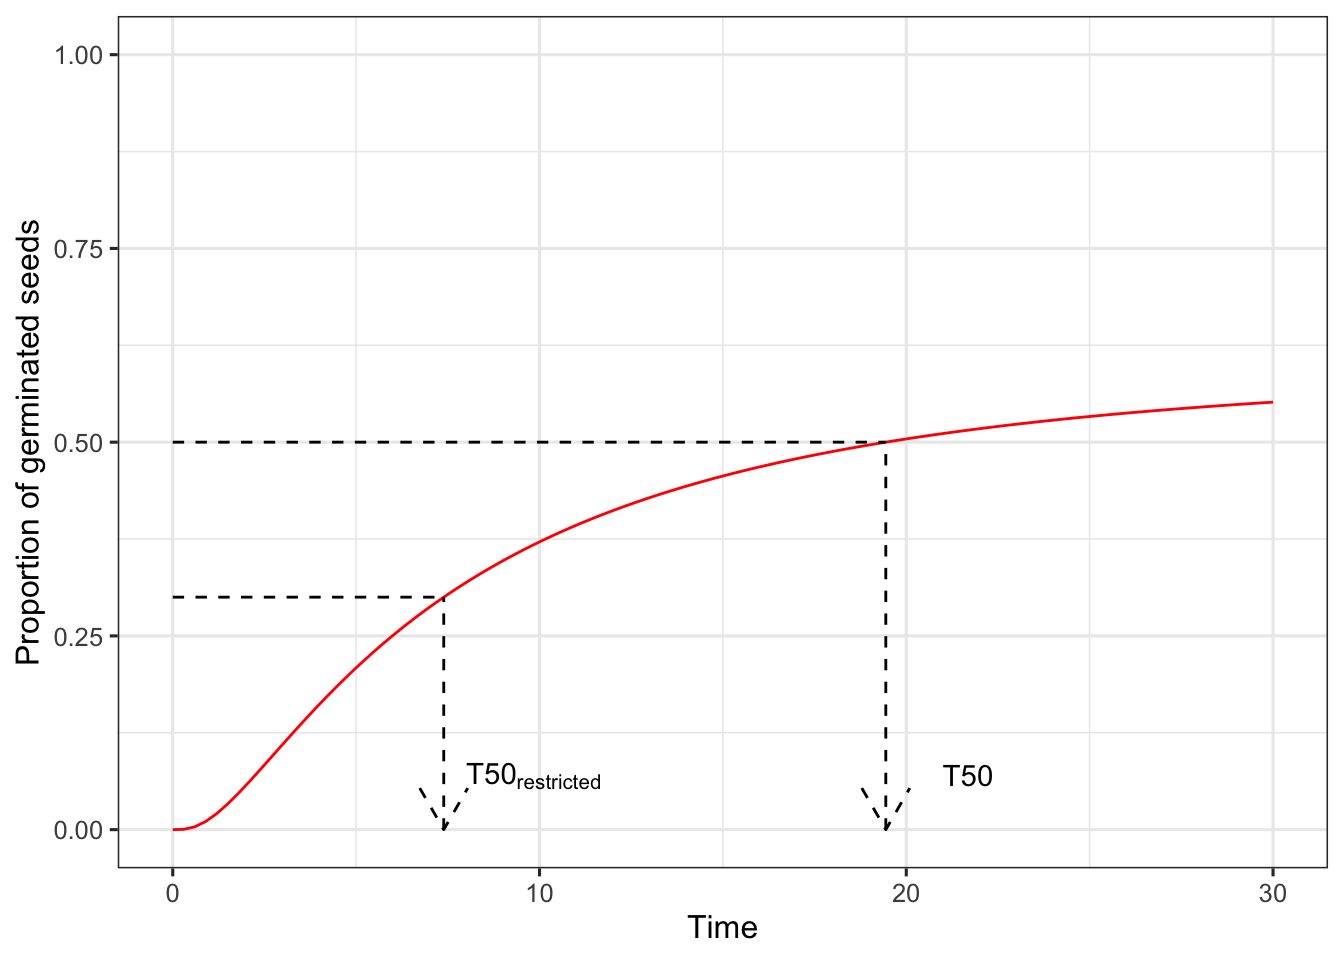
\includegraphics[width=0.9\linewidth]{_seedGerminationTutorial_files/figure-latex/unnamed-chunk-49-1}

\hypertarget{germinationemergence-rates}{%
\subsection{Germination/emergence rates}\label{germinationemergence-rates}}

The quantiles of germination times (e.g., T10, T30 or T50) are very common measures of germination velocity, although they may be rather counterintuitive, because a high germination time implies low velocity. Another common measure of velocity is the Germination Rate, that is the inverse of germination time (e.g., GR10 = 1/T10).

The quantiles of germination rates (e.g., GR10, GR30, GR50\ldots) represents the daily progress to germination for a given subpopulation and they are used as the basis for hydro-thermal-time modelling. Therefore, their determination for a seed lot is also very relevant.

\hypertarget{getting-the-quantiles-with-drcte}{%
\section{Getting the quantiles with `drcte'}\label{getting-the-quantiles-with-drcte}}

\hypertarget{parametric-models}{%
\subsection{Parametric models}\label{parametric-models}}

In a previous post we have used the code below to fit a log-logistic time-to-event model to the germination data for three species of the Verbascum genus:

\begin{Shaded}
\begin{Highlighting}[]
\FunctionTok{library}\NormalTok{(drcte)}
\FunctionTok{library}\NormalTok{(drcSeedGerm)}
\FunctionTok{data}\NormalTok{(verbascum)}
\NormalTok{mod1 }\OtherTok{\textless{}{-}} \FunctionTok{drmte}\NormalTok{(nSeeds }\SpecialCharTok{\textasciitilde{}}\NormalTok{ timeBef }\SpecialCharTok{+}\NormalTok{ timeAf, }\AttributeTok{fct =} \FunctionTok{LL.3}\NormalTok{(),}
             \AttributeTok{curveid =}\NormalTok{ Species, }\AttributeTok{data =}\NormalTok{ verbascum)}
\FunctionTok{summary}\NormalTok{(mod1, }\AttributeTok{units =}\NormalTok{ Dish)}
\DocumentationTok{\#\# }
\DocumentationTok{\#\# Model fitted: Log{-}logistic (ED50 as parameter) with lower limit at 0}
\DocumentationTok{\#\# }
\DocumentationTok{\#\# Robust estimation: Cluster robust sandwich SEs }
\DocumentationTok{\#\# }
\DocumentationTok{\#\# Parameter estimates:}
\DocumentationTok{\#\# }
\DocumentationTok{\#\#               Estimate Std. Error  t value  Pr(\textgreater{}|t|)    }
\DocumentationTok{\#\# b:arcturus   {-}9.930005   1.111135  {-}8.9368 4.286e{-}16 ***}
\DocumentationTok{\#\# b:blattaria  {-}7.198025   0.575290 {-}12.5120 \textless{} 2.2e{-}16 ***}
\DocumentationTok{\#\# b:creticum  {-}11.033749   0.943374 {-}11.6961 \textless{} 2.2e{-}16 ***}
\DocumentationTok{\#\# d:arcturus    0.356648   0.047915   7.4433 3.715e{-}12 ***}
\DocumentationTok{\#\# d:blattaria   0.840064   0.025593  32.8242 \textless{} 2.2e{-}16 ***}
\DocumentationTok{\#\# d:creticum    0.969990   0.017290  56.1015 \textless{} 2.2e{-}16 ***}
\DocumentationTok{\#\# e:arcturus   12.059189   0.486010  24.8126 \textless{} 2.2e{-}16 ***}
\DocumentationTok{\#\# e:blattaria   4.031763   0.199590  20.2002 \textless{} 2.2e{-}16 ***}
\DocumentationTok{\#\# e:creticum    3.200655   0.103161  31.0259 \textless{} 2.2e{-}16 ***}
\DocumentationTok{\#\# {-}{-}{-}}
\DocumentationTok{\#\# Signif. codes:  0 \textquotesingle{}***\textquotesingle{} 0.001 \textquotesingle{}**\textquotesingle{} 0.01 \textquotesingle{}*\textquotesingle{} 0.05 \textquotesingle{}.\textquotesingle{} 0.1 \textquotesingle{} \textquotesingle{} 1}
\end{Highlighting}
\end{Shaded}

It may be useful to rank the species in terms of their germination velocity and, to that purpose, we could estimate the times to 30\% and 50\% germination (T30 and T50), that are the 30\textsuperscript{th} and 50\textsuperscript{th} percentiles of the time-to-event distribution. We can use the \texttt{quantile()} method, where the probability levels are passed in as the vector `probs':

\begin{Shaded}
\begin{Highlighting}[]
\FunctionTok{quantile}\NormalTok{(mod1, }\AttributeTok{probs =} \FunctionTok{c}\NormalTok{(}\FloatTok{0.3}\NormalTok{, }\FloatTok{0.5}\NormalTok{))}
\DocumentationTok{\#\# }
\DocumentationTok{\#\# Estimated quantiles}
\DocumentationTok{\#\# }
\DocumentationTok{\#\#               Estimate       SE}
\DocumentationTok{\#\# arcturus:30\%   14.2634 0.992685}
\DocumentationTok{\#\# arcturus:50\%       NaN      NaN}
\DocumentationTok{\#\# blattaria:30\%   3.7156 0.106048}
\DocumentationTok{\#\# blattaria:50\%   4.2536 0.118515}
\DocumentationTok{\#\# creticum:30\%    2.9759 0.058279}
\DocumentationTok{\#\# creticum:50\%    3.2187 0.059480}
\end{Highlighting}
\end{Shaded}

We may note that the T50 is not estimable with \emph{Verbascum arcturus}, as the maximum germinated proportion (\emph{d} parameter for the time-to-event model above) is 0.36. Standard errors are obtained by using the delta method and they are invalid whenever the experimental units (seeds) are clustered within containers, such as the Petri dishes.

For all these cases, we should prefer cluster-robust standard errors (Zeileis et al.~2020), which can be obtained by setting the extra argument `robust = TRUE' and providing a clustering variable as the \texttt{units} argument. By setting `interval = TRUE' we can also obtain confidence intervals for the desired probability level (0.95, by default).

\begin{Shaded}
\begin{Highlighting}[]
\FunctionTok{quantile}\NormalTok{(mod1, }\AttributeTok{probs =} \FunctionTok{c}\NormalTok{(}\FloatTok{0.3}\NormalTok{, }\FloatTok{0.5}\NormalTok{), }\AttributeTok{robust =}\NormalTok{ T,}
         \AttributeTok{units =}\NormalTok{ Dish,}
         \AttributeTok{interval =}\NormalTok{ T)}
\DocumentationTok{\#\# }
\DocumentationTok{\#\# Estimated quantiles}
\DocumentationTok{\#\# }
\DocumentationTok{\#\#               Estimate       SE   Lower   Upper}
\DocumentationTok{\#\# arcturus:30\%   14.2634 0.755294 12.7830 15.7437}
\DocumentationTok{\#\# arcturus:50\%       NaN      NaN     NaN     NaN}
\DocumentationTok{\#\# blattaria:30\%   3.7156 0.187503  3.3481  4.0831}
\DocumentationTok{\#\# blattaria:50\%   4.2536 0.209853  3.8423  4.6649}
\DocumentationTok{\#\# creticum:30\%    2.9759 0.085151  2.8090  3.1428}
\DocumentationTok{\#\# creticum:50\%    3.2187 0.104743  3.0134  3.4240}
\end{Highlighting}
\end{Shaded}

We may note that cluster robust standard errors are higher than naive standard errors: the seed in the same Petri dish are correlated and, thus, they do not contribute full information.

If we are interested in the germination rates G30 and G50, we can set the argument `rate = T', as shown in the box below.

\begin{Shaded}
\begin{Highlighting}[]
\FunctionTok{quantile}\NormalTok{(mod1, }\AttributeTok{probs =} \FunctionTok{c}\NormalTok{(}\FloatTok{0.3}\NormalTok{, }\FloatTok{0.5}\NormalTok{), }\AttributeTok{robust =}\NormalTok{ T,}
         \AttributeTok{units =}\NormalTok{ Dish,}
         \AttributeTok{interval =}\NormalTok{ T, }\AttributeTok{rate =}\NormalTok{ T)}
\DocumentationTok{\#\# }
\DocumentationTok{\#\# Estimated quantiles}
\DocumentationTok{\#\# }
\DocumentationTok{\#\#               Estimate        SE    Lower    Upper}
\DocumentationTok{\#\# arcturus:30\%   0.07011 0.0037126 0.062833 0.077386}
\DocumentationTok{\#\# arcturus:50\%   0.00000 0.0000000 0.000000 0.000000}
\DocumentationTok{\#\# blattaria:30\%  0.26914 0.0135819 0.242519 0.295759}
\DocumentationTok{\#\# blattaria:50\%  0.23510 0.0115987 0.212364 0.257830}
\DocumentationTok{\#\# creticum:30\%   0.33604 0.0096153 0.317191 0.354882}
\DocumentationTok{\#\# creticum:50\%   0.31069 0.0101106 0.290872 0.330505}
\end{Highlighting}
\end{Shaded}

\hypertarget{parametric-models-with-environmental-covariates}{%
\subsection{Parametric models with environmental covariates}\label{parametric-models-with-environmental-covariates}}

If we have fitted a hydro-thermal time model or other models with an environmental covariate, we can also use the \texttt{quantile()} method, and pass a value for that covariate, as shown in the code below.

\begin{Shaded}
\begin{Highlighting}[]
\CommentTok{\# Parametric model with environmental covariate}
\FunctionTok{data}\NormalTok{(rape)}
\NormalTok{modTE }\OtherTok{\textless{}{-}} \FunctionTok{drmte}\NormalTok{(nSeeds }\SpecialCharTok{\textasciitilde{}}\NormalTok{ timeBef }\SpecialCharTok{+}\NormalTok{ timeAf }\SpecialCharTok{+}\NormalTok{ Psi,}
            \AttributeTok{data =}\NormalTok{ rape, }\AttributeTok{fct =} \FunctionTok{HTLL}\NormalTok{())}
\FunctionTok{quantile}\NormalTok{(modTE, }\AttributeTok{Psi =} \DecValTok{0}\NormalTok{, }
         \AttributeTok{probs =} \FunctionTok{c}\NormalTok{(}\FloatTok{0.05}\NormalTok{, }\FloatTok{0.10}\NormalTok{, }\FloatTok{0.15}\NormalTok{, }\FloatTok{0.21}\NormalTok{), }
         \AttributeTok{restricted =}\NormalTok{ F, }\AttributeTok{rate =}\NormalTok{ T, }\AttributeTok{robust =}\NormalTok{ T,}
         \AttributeTok{interval =}\NormalTok{ T)}
\DocumentationTok{\#\# }
\DocumentationTok{\#\# Estimated quantiles}
\DocumentationTok{\#\# }
\DocumentationTok{\#\#       Estimate      SE  Lower  Upper}
\DocumentationTok{\#\# 1:5\%    1.5861 0.22621 1.1428 2.0295}
\DocumentationTok{\#\# 1:10\%   1.5562 0.21060 1.1435 1.9690}
\DocumentationTok{\#\# 1:15\%   1.5331 0.20063 1.1399 1.9263}
\DocumentationTok{\#\# 1:21\%   1.5090 0.19183 1.1330 1.8850}
\end{Highlighting}
\end{Shaded}

The environmental covariate only accepts a single value; in order to vectorise, we need to use the \texttt{lapply()} function, as shown below.

\begin{Shaded}
\begin{Highlighting}[]
\CommentTok{\# This is to vectorise on Psi}
\NormalTok{psiList }\OtherTok{\textless{}{-}} \FunctionTok{seq}\NormalTok{(}\SpecialCharTok{{-}}\DecValTok{1}\NormalTok{, }\DecValTok{0}\NormalTok{, }\FloatTok{0.25}\NormalTok{)}
\FunctionTok{names}\NormalTok{(psiList) }\OtherTok{\textless{}{-}} \FunctionTok{as.character}\NormalTok{(psiList)}
\FunctionTok{lapply}\NormalTok{(psiList, }
       \ControlFlowTok{function}\NormalTok{(x) }\FunctionTok{quantile}\NormalTok{(modTE, }\AttributeTok{Psi =}\NormalTok{ x, }
                            \AttributeTok{probs =} \FunctionTok{c}\NormalTok{(}\FloatTok{0.05}\NormalTok{, }\FloatTok{0.10}\NormalTok{, }\FloatTok{0.15}\NormalTok{, }\FloatTok{0.21}\NormalTok{),}
                            \AttributeTok{restricted =}\NormalTok{ F, }\AttributeTok{rate =}\NormalTok{ T,}
                            \AttributeTok{interval =} \StringTok{"delta"}\NormalTok{, }
                            \AttributeTok{units =}\NormalTok{ rape}\SpecialCharTok{$}\NormalTok{Dish, }
                            \AttributeTok{display =}\NormalTok{ F))}
\DocumentationTok{\#\# $\textasciigrave{}{-}1\textasciigrave{}}
\DocumentationTok{\#\#         Estimate         SE         Lower      Upper}
\DocumentationTok{\#\# 1:5\%  0.10860038 0.05566722 {-}0.0005053734 0.21770613}
\DocumentationTok{\#\# 1:10\% 0.07869462 0.03741665  0.0053593346 0.15202991}
\DocumentationTok{\#\# 1:15\% 0.05555279 0.02674483  0.0031338819 0.10797171}
\DocumentationTok{\#\# 1:21\% 0.03145638 0.01993608 {-}0.0076176237 0.07053039}
\DocumentationTok{\#\# }
\DocumentationTok{\#\# $\textasciigrave{}{-}0.75\textasciigrave{}}
\DocumentationTok{\#\#        Estimate         SE     Lower     Upper}
\DocumentationTok{\#\# 1:5\%  0.4779833 0.08302599 0.3152553 0.6407112}
\DocumentationTok{\#\# 1:10\% 0.4480775 0.06331212 0.3239880 0.5721670}
\DocumentationTok{\#\# 1:15\% 0.4249357 0.05037871 0.3261952 0.5236762}
\DocumentationTok{\#\# 1:21\% 0.4008393 0.03876416 0.3248629 0.4768157}
\DocumentationTok{\#\# }
\DocumentationTok{\#\# $\textasciigrave{}{-}0.5\textasciigrave{}}
\DocumentationTok{\#\#        Estimate         SE     Lower     Upper}
\DocumentationTok{\#\# 1:5\%  0.8473662 0.11816778 0.6157616 1.0789708}
\DocumentationTok{\#\# 1:10\% 0.8174604 0.09946283 0.6225169 1.0124040}
\DocumentationTok{\#\# 1:15\% 0.7943186 0.08738918 0.6230390 0.9655982}
\DocumentationTok{\#\# 1:21\% 0.7702222 0.07670819 0.6198769 0.9205675}
\DocumentationTok{\#\# }
\DocumentationTok{\#\# $\textasciigrave{}{-}0.25\textasciigrave{}}
\DocumentationTok{\#\#       Estimate        SE     Lower    Upper}
\DocumentationTok{\#\# 1:5\%  1.216749 0.1559175 0.9111565 1.522342}
\DocumentationTok{\#\# 1:10\% 1.186843 0.1380349 0.9162999 1.457387}
\DocumentationTok{\#\# 1:15\% 1.163702 0.1265389 0.9156899 1.411713}
\DocumentationTok{\#\# 1:21\% 1.139605 0.1163701 0.9115239 1.367686}
\DocumentationTok{\#\# }
\DocumentationTok{\#\# $\textasciigrave{}0\textasciigrave{}}
\DocumentationTok{\#\#       Estimate        SE    Lower    Upper}
\DocumentationTok{\#\# 1:5\%  1.586132 0.1947646 1.204400 1.967864}
\DocumentationTok{\#\# 1:10\% 1.556226 0.1774564 1.208418 1.904034}
\DocumentationTok{\#\# 1:15\% 1.533084 0.1663240 1.207095 1.859073}
\DocumentationTok{\#\# 1:21\% 1.508988 0.1564488 1.202354 1.815622}
\end{Highlighting}
\end{Shaded}

\hypertarget{non-parametric-npmle-models}{%
\subsection{Non-parametric (NPMLE) models}\label{non-parametric-npmle-models}}

The \texttt{quantile()} method can also be used to make predictions from NPMLE fits. This method works by assuming that the events are evenly scattered within each inspection interval (`interpolation method'). Inferences need to be explicitly requested by using setting `interval = T'; in this case, standard errors are estimated by using a resampling approach, that is performed at the group level, whenever a grouping variable is provided, by way of the `units' argument (Davison and Hinkley, 1997).

\begin{Shaded}
\begin{Highlighting}[]
\NormalTok{mod2 }\OtherTok{\textless{}{-}} \FunctionTok{drmte}\NormalTok{(nSeeds }\SpecialCharTok{\textasciitilde{}}\NormalTok{ timeBef }\SpecialCharTok{+}\NormalTok{ timeAf, }\AttributeTok{fct =} \FunctionTok{NPMLE}\NormalTok{(),}
             \AttributeTok{curveid =}\NormalTok{ Species, }\AttributeTok{data =}\NormalTok{ verbascum)}
\FunctionTok{quantile}\NormalTok{(mod2, }\AttributeTok{probs =} \FunctionTok{c}\NormalTok{(}\FloatTok{0.3}\NormalTok{, }\FloatTok{0.5}\NormalTok{), }\AttributeTok{robust =}\NormalTok{ T, }\AttributeTok{units =}\NormalTok{ Dish,}
         \AttributeTok{interval =}\NormalTok{ T, }\AttributeTok{rate =}\NormalTok{ T)}
\DocumentationTok{\#\# }
\DocumentationTok{\#\# }
\DocumentationTok{\#\# }
\DocumentationTok{\#\# }
\DocumentationTok{\#\# Estimated quantiles}
\DocumentationTok{\#\# (cluster robust bootstrap{-}based inference)}
\DocumentationTok{\#\# }
\DocumentationTok{\#\#                 n       Mean   Median        SE   Lower    Upper}
\DocumentationTok{\#\# arcturus.30\%  999 0.04215854 0.067385 0.0367409 0.00000 0.085837}
\DocumentationTok{\#\# arcturus.50\%  999 0.00047593 0.000000 0.0056696 0.00000 0.000000}
\DocumentationTok{\#\# blattaria.30\% 999 0.26933051 0.268456 0.0180207 0.23961 0.308415}
\DocumentationTok{\#\# blattaria.50\% 999 0.23279718 0.230530 0.0131552 0.21341 0.263740}
\DocumentationTok{\#\# creticum.30\%  999 0.34397841 0.343750 0.0195091 0.31087 0.379032}
\DocumentationTok{\#\# creticum.50\%  999 0.30314443 0.302198 0.0117692 0.28139 0.326935}
\end{Highlighting}
\end{Shaded}

For KDE models, quantiles are calculated from the time-to-event curve by using a bisection method. However, we are still unsure about the most reliable way to obtain standard errors and, for this reason, inferences are not provided with this type of non-parametric models.

\hypertarget{quantiles-and-effective-doses-ed}{%
\section{Quantiles and Effective Doses (ED)}\label{quantiles-and-effective-doses-ed}}

Quantiles for time-to-event data resamble Effective Doses (ED) for dose-response data, although we discourage the use of this latter term, as the time-to-event curve is a cumulative probability function based on time, that is not a `dose' in strict terms. However, the concept is similar: we need to find the stimulus (time) that permits to obtain a certain response (germination/emergence). Considering such similarity, we decided to define the \texttt{ED()} method for `drcte' objects, that is compatible with the \texttt{ED()} method for `drc' objects. However, for seed germination/emergence data, we strongly favor the use of the \texttt{quantile()} method.

\hypertarget{fitting-germination-models-in-two-steps}{%
\chapter{Fitting germination models in two steps}\label{fitting-germination-models-in-two-steps}}

In the previous sections I have shown how to fit time-to-event curves to seed germination data. I have also shown that these curves can be modified to include the effect of external factors (e.g., the species) or covariates (e.g., temperature or humidity content in the substrate), which brought us to the definition of hydro-time, thernal-time or hydro-thermal-time models. So far, in this tutorial, we have fitted these modified time-to-event curves in `one-step', i.e., we started from the germination data, fitted the selected model and retrieved the estimates of model parameters. In such a one-step approach, we showed that one problem was that, most of the times, seeds were not independent, but, they were clustered within Petri dishes, trays, boxes or other containers. Such a clustering, if not appropriately accounted for, brakes the independence assumption that is made by most linear and nonlinear models, invalidating the inferences based on those models.

So far, we have accounted for the above mentioned clustering by using cluster robust standard errors, which are easily calculated within the `drcte' package. However, we should also say that one-step model fitting may often be complex, particularly when we have to deal with a high number of seeds, complex models and multi-tier experimental designs. In order to avoid such complexities, we might like to follow a different approach, that is accomplished in two-steps. Let's consider an example where we have performed germination assays where seeds have been submitted to 10 different treatment levels: instead of building a time-to-event model that contains the treatment as an external factor, we could:

\begin{enumerate}
\def\labelenumi{\arabic{enumi}.}
\tightlist
\item
  independently fit a different time-to-event curve to the germination data for each treatment level, so that we have ten independent time-to-event curves;
\item
  derive from each curve a summary statistic of interest, such as the germination rate for the 50-th percentile (GR50; see earlier in this tutorial);
\item
  fit, e.g., a thermal-time model to those derived statistics (second step of data analyses).
\end{enumerate}

Fitting models in two-steps has always been a common practice in agriculture/biology (see, e.g., multienvironment genotype experiments): it is usually simpler, quicker and requires lower computing power than one-step fitting. The drawback is that some infomation may be lost between the two steps, and, for this reason, one-step and two-steps model fitting do not necessarily lead to the same results. But, we'll make this point later.

Let's show some examples of this two-steps approach.

\hypertarget{fitting-linear-models-in-two-steps}{%
\section{Fitting linear models in two steps}\label{fitting-linear-models-in-two-steps}}

(yet to be done)

\hypertarget{fitting-non-linear-threshold-models-in-two-steps}{%
\section{Fitting non-linear threshold models in two steps}\label{fitting-non-linear-threshold-models-in-two-steps}}

\hypertarget{definition-of-threshold-models}{%
\subsection{Definition of threshold models}\label{definition-of-threshold-models}}

Threshold models are used to describe a relationship where the response variable changes abruptly, following a small change in the predictor. A typical threshold model looks like that in the Figure below, where we see three threshold levels:

\begin{enumerate}
\def\labelenumi{\arabic{enumi}.}
\tightlist
\item
  \(X1 = 5.5\): at this threshold, the response changes abruptly from `flat' to linearly increasing;
\item
  \(X2 = 23.1\): at this threshold, the response changes abruptly from linearly increasing to linearly decreasing;
\item
  \(X3 = 37.2\): at this threshold, the response changes abruptly from linearly decreasing to `flat'.
\end{enumerate}

You may recognise a `broken-stick' pattern, although threshold models can also be curvilinear, as we will see later.

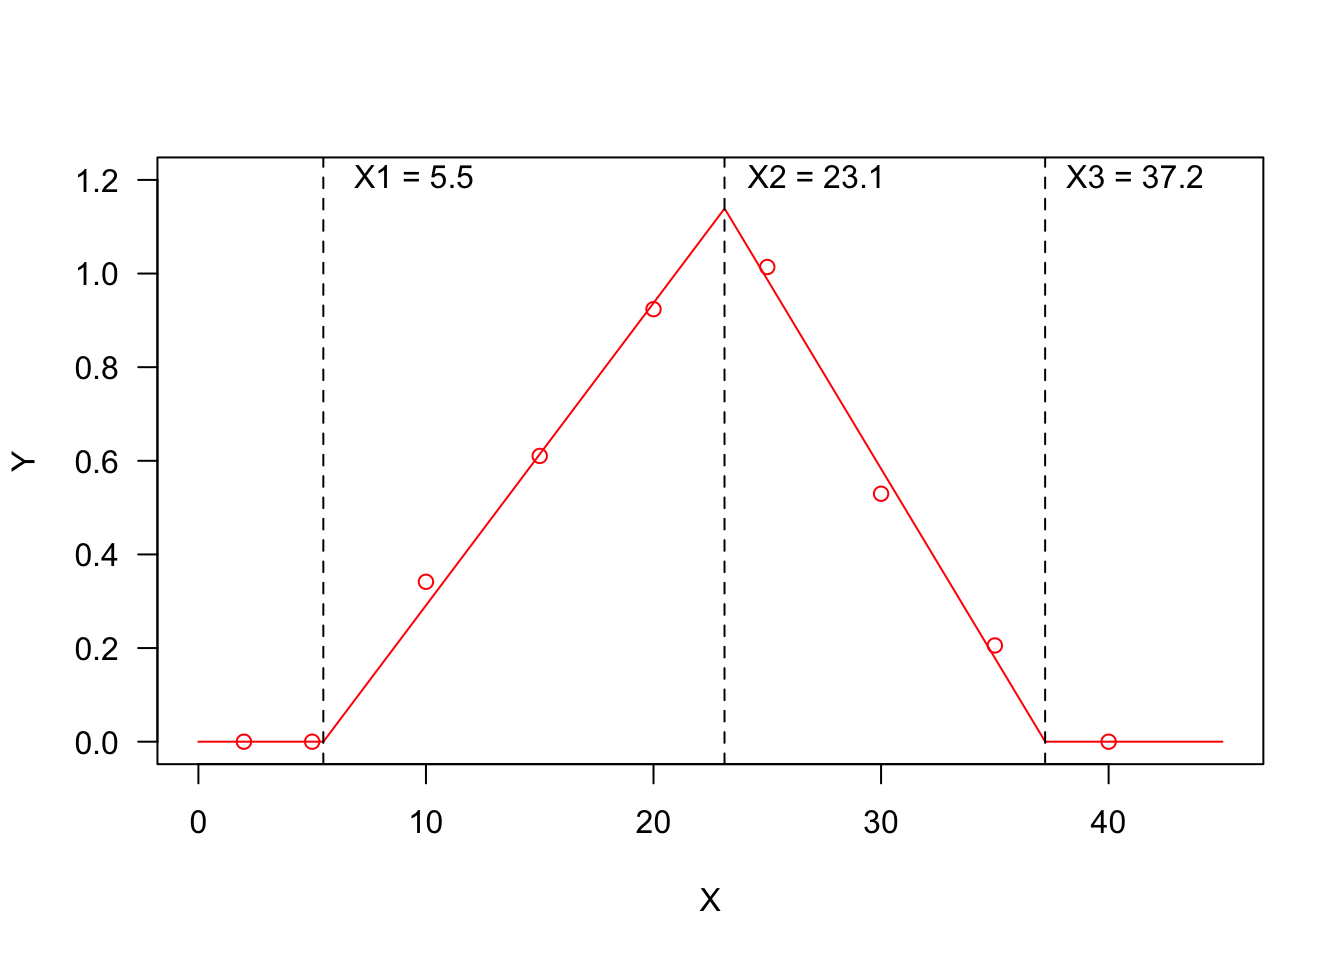
\includegraphics[width=0.9\linewidth]{_seedGerminationTutorial_files/figure-latex/unnamed-chunk-57-1}

I have already considered threshold models in a previous post (\href{https://www.statforbiology.com/2021/stat_seedgermination_htt2step/}{see here}) and I have already mentioned that thermal-time, hydro-time and hydro-thermal-time models for seed germination can also be cast as threshold models; if we consider, e.g., the Germination Rate (GR) as the response variable and the environmental temperature as the predictor, the relationship could be very close to that represented in Figure 1 and the three thresholds would, respectively, be the \emph{base temperature} (T\_b\_), the \emph{optimal temperature} (T\_o\_) and the \emph{ceiling temperature} (T\_c\_). On the other hand, if we consider the effect of soil humidity on GR, we should expect a response pattern with only one threshold, i.e.~the \emph{base water potential} level (e.g.~the first half of the figure above, up to the maximum response level).

\hypertarget{a-possibly-incomplete-list-of-threshold-models}{%
\subsection{A (possibly incomplete) list of threshold models}\label{a-possibly-incomplete-list-of-threshold-models}}

I have made a review of literature, searching for all threshold models that have been used so far in seed germination studies. For all those models, I have built the related R functions, together with self-starting routines, which can be used for nonlinear regression fitting with the \texttt{drm()} function in the \texttt{drc} package (Ritz et al., 2019). The availability of self-starting routines will free you from the hassle of having to provide initial guesses for model parameters. All these R functions are available within the \texttt{drcSeedGerm} package (Onofri et al., 2018) and their names, with links to the relevant parts of the appendix to this post are:

\begin{enumerate}
\def\labelenumi{\arabic{enumi}.}
\tightlist
\item
  \protect\hyperlink{grpsilin---grt.gh}{GRPsi.Lin() - GRT.GH()}
\item
  \protect\hyperlink{grpsipol---grpsipol2}{GRPsi.Pol() - GRPsi.Pol2()}
\item
  \protect\hyperlink{pmaxpsi1-and-pmaxt1}{PmaxPsi1() - PmaxT1()}
\item
  \protect\hyperlink{grt.bs}{GRT.BS()}
\item
  \protect\hyperlink{grt.rf}{GRT.RF()}
\item
  \protect\hyperlink{grt.m}{GRT.M()}
\item
  \protect\hyperlink{grt.ex}{GRT.Ex()}
\item
  \protect\hyperlink{grt.yl}{GRT.YL()}
\end{enumerate}

It may be helpful to look at the shapes of the above models in the Figure below, while the equations are motivated in the appendix, at the end of this post.

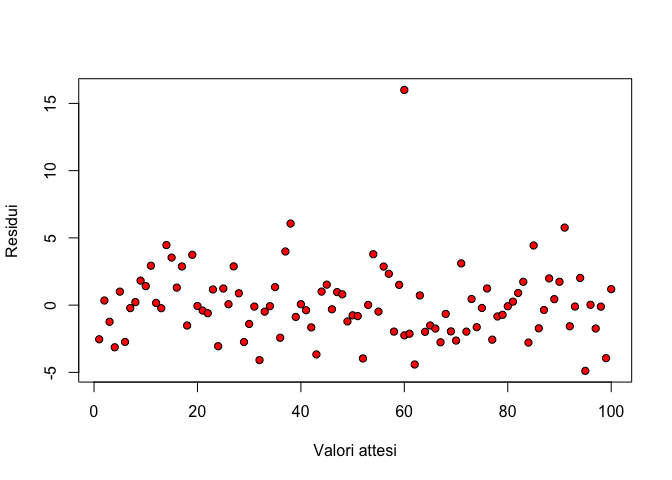
\includegraphics[width=0.9\linewidth]{_seedGerminationTutorial_files/figure-latex/unnamed-chunk-58-1}

Now, let's look at a few examples of two-steps fitting. But, before working through this, you will need to install and load the \texttt{drcSeedGerm} package, by using the code below.

\begin{Shaded}
\begin{Highlighting}[]
\CommentTok{\# installing drcSeedGerm package, if not yet available}
\CommentTok{\# library(devtools)}
\CommentTok{\# install\_github("onofriandreapg/drcSeedGerm")}

\CommentTok{\# loading package}
\FunctionTok{library}\NormalTok{(drcSeedGerm)}
\FunctionTok{library}\NormalTok{(tidyverse)}
\FunctionTok{library}\NormalTok{(lmtest)}
\FunctionTok{library}\NormalTok{(sandwich)}
\end{Highlighting}
\end{Shaded}

\hypertarget{description-of-models}{%
\subsection{Description of models}\label{description-of-models}}

\hypertarget{grpsilin---grt.gh}{%
\subsubsection{GRPsiLin() - GRT.GH()}\label{grpsilin---grt.gh}}

The equation behind \texttt{GRPsiLin()} has been used to describe the effect of environmental humidity (\(\Psi\), in MPa) on germination rate (Bradford, 2002):

\[GR = \frac{\max\left[\Psi, \Psi_b\right] - \Psi_b}{\theta_H}\]

The parameter \(\Psi_b\) is the \emph{base water potential} (in MPa), representing the minimum level of humidity in the substrate to trigger the germination process. The other parameter \(\theta_H\) (in MPa day or MPa hour) is the hydro-time constant.

A totally similar equation (with different parameter names) has been used by Garcia-Huidobro et al (1982), to describe the effect of sub-optimal temperatures (T in °C) on the germination rate:

\[GR = \frac{\max \left[T, T_b\right] - T_b}{\theta_T}\]

where \(T_b\) is the base temperature and \(\theta_T\) is the thermal time (in °C d). This second model is available \texttt{GRT.GH()}.

\begin{Shaded}
\begin{Highlighting}[]
\CommentTok{\# sample code (not executed)}
\CommentTok{\# Tlev \textless{}{-} c(2, 5, 10, 15, 20, 25)}
\CommentTok{\# GR \textless{}{-} c(0, 0, 0.21, 0.49, 0.68, 0.86)}
\CommentTok{\# modGH \textless{}{-} drm(GR \textasciitilde{} Tlev, fct = GRT.GH())}
\CommentTok{\# library(sandwich); library(lmtest)}
\CommentTok{\# coeftest(modGH, vcov = sandwich)}
\CommentTok{\# plot(modGH, log="", xlim = c(0, 25), legendPos = c(5, 1.2),}
\CommentTok{\#      xlab = "Temperature (°C)")}
\end{Highlighting}
\end{Shaded}

\hypertarget{grpsipol---grpsipol2}{%
\subsubsection{GRPsiPol() - GRPsiPol2()}\label{grpsipol---grpsipol2}}

In my experience, I have found that the relationship between GR and water potential in the substrate may, sometimes, be curvilinear. For these situations, I have successfully used the following equations:

\[GR = \frac{\max\left[\Psi,\Psi_b\right]^2 - \Psi^2_b}{\theta_H}\]

and:

\[GR = \frac{\left(\max\left[\Psi, \Psi_b\right] - \Psi_b \right)^2}{ \theta_H }\]

Both models can be fitted in R, by using the two functions \texttt{GRPsi.Pol()} and \texttt{GRPsi.Pol2()}

\begin{Shaded}
\begin{Highlighting}[]
\CommentTok{\# sample code (not executed)}
\CommentTok{\# Psi \textless{}{-} c({-}2, {-}1.5, {-}1.2, {-}1, {-}0.8, {-}0.6, {-}0.4, {-}0.25,}
\CommentTok{\#          {-}0.12, {-}0.06, {-}0.03, 0)}
\CommentTok{\# GR \textless{}{-} c(0, 0, 0, 0, 0.0585, 0.094, 0.1231, 0.1351,}
\CommentTok{\#         0.1418, 0.1453, 0.1458, 0.1459)}
\CommentTok{\# Psi2 \textless{}{-} c({-}0.5, {-}0.6, {-}0.7, {-}0.8, {-}0.9, {-}1, {-}1.1, {-}1.2,}
\CommentTok{\#           {-}1.5)}
\CommentTok{\# GR2 \textless{}{-} c(1.4018, 1.0071, 0.5614, 0.3546, 0.2293, 0, 0,}
\CommentTok{\#          0, 0)}
\CommentTok{\# }
\CommentTok{\# }
\CommentTok{\# modHT \textless{}{-} drm(GR \textasciitilde{} Psi, fct = GRPsiPol())}
\CommentTok{\# modHT2 \textless{}{-} drm(GR2 \textasciitilde{} Psi2, fct = GRPsiPol2())}
\CommentTok{\# par(mfrow = c(1,2))}
\CommentTok{\# plot(modHT, log="", legendPos = c({-}1.5, 0.15), }
\CommentTok{\#      ylim = c(0, 0.20), xlab = "Water potential (MPa)")}
\CommentTok{\# plot(modHT2, log="", legendPos=c({-}1.3, 1), }
\CommentTok{\#      xlab = "Water potential (MPa)")}
\end{Highlighting}
\end{Shaded}

\hypertarget{pmaxpsi1-and-pmaxt1}{%
\subsubsection{PmaxPsi1() and PmaxT1()}\label{pmaxpsi1-and-pmaxt1}}

All the previous models tend to go up to infinity when the predictor value (temperature or water potential) goes to infinity. In some instances, we may need an asymptotic model, to describe the response of the maximum proportion of germinated seeds to soil humidity (Onofri et al., 2018).

In practice, we could use a shifted exponential model:

\[ \pi = G \, \left[ 1 - exp \left( \frac{ \max\left[\Psi, \Psi_b\right] - \Psi_b }{\sigma} \right) \right]\]

where \(\pi\) is the proportion of germinated seeds, \(G\) is the fraction of non-germinable seeds (e.g., dormant seeds) and \(\sigma\) describes how quickly the population of seeds responds to increased humidity in the substrate. This model can be fitted by using the R function the self-starters \texttt{PmaxPsi1()}.

If we reverse the sign of \(\sigma\) in the previous equation, we obtain a decreasing trend, which might be useful to describe the effect of super-optimal temperatures on the proportion of germinated seeds, going down to 0 at the ceiling temperature threshold. Also this model is available in R, under the name \texttt{PmaxT1()}. \texttt{PmaxPsi1()} \texttt{PmaxT1()} are two equivalent R functions, apart from the name of model parameters.

\begin{Shaded}
\begin{Highlighting}[]
\CommentTok{\# sample code (not executed)}
\CommentTok{\# par(mfrow = c(1,2))}
\CommentTok{\# \# Pmax vs Psi}
\CommentTok{\# Psi \textless{}{-} seq({-}2.2, 0, by = 0.2)}
\CommentTok{\# Pmax \textless{}{-} c(0, 0, 0.076, 0.413, 0.514, 0.643, 0.712,}
\CommentTok{\#           0.832, 0.865, 0.849, 0.89, 0.90)}
\CommentTok{\# mod \textless{}{-} drm(Pmax \textasciitilde{} Psi, fct = PmaxPsi1())}
\CommentTok{\# plot(mod, log = "", xlab = "Water potential (MPa)", }
\CommentTok{\#      ylab = "Proportion of germinating seeds")}
\CommentTok{\# }
\CommentTok{\# \# Pmax vs temperature}
\CommentTok{\# Tval \textless{}{-} c(0, 2.5, 5, 7.5, 10, 12.5, 15, 17.5,}
\CommentTok{\#           20, 22.5, 25, 27.5, 30, 32.5, 35)}
\CommentTok{\# Pmax2 \textless{}{-} c(0.79, 0.81, 0.807, 0.776, 0.83,}
\CommentTok{\#            0.73, 0.744, 0.73, 0.828, 0.818,}
\CommentTok{\#            0.805, 0.706, 0.41, 0.002, 0)}
\CommentTok{\# mod2 \textless{}{-} drm(Pmax2 \textasciitilde{} Tval, fct = PmaxT1())}
\CommentTok{\# plot(mod2, log = "", xlab = "Temperature (°C)", }
\CommentTok{\#      ylab = "Proportion of germinating seeds")}
\end{Highlighting}
\end{Shaded}

\hypertarget{grt.bs}{%
\subsubsection{GRT.BS()}\label{grt.bs}}

A broken-stick trend, as the one depicted in the first Figure above was used by Alvarado and Bradford (2002) to model the effect of temperature on the germination rate. Their equation is:

\[GR = \frac{\max \left[\min \left[T,T_o \right], Tb \right] - T_b}{\theta_{T}} \, \left\{ 1 - k \left( \max \left[ T,T_o \right] - T_o \right) \right\}\]
The right factor is only meaningful when it is positive, that happens when \(T < T_c\), i.e.~when the environmental temperature is lower than the ceiling temperature. On this basis, the ceiling temperature is equal to:

\[ T_c = \frac{1}{k} + T_o\]

The above equation can be easily fitted with the \texttt{GRT.BS()} function in the `drcSeedGerm' package. We have also implemented the reparameterised equation, where the parameter `k' is replaced with \(1/(T_c - T_b)\):

\[GR = \frac{\min \left[T,T_o \right] - T_b}{\theta_{T}} \, \left\{ 1 - \frac {\min \left[\max \left[ T,T_o \right], T_c \right] - T_o}{T_c - T_o} \right\}\]

This reparameterised equation is available as \texttt{GRT.BSb()}; it is handy, because the ceiling temperature is included as a parameter, but its fitting properties are not as good as those of the previous equation.

\begin{Shaded}
\begin{Highlighting}[]
\CommentTok{\# sample code}
\CommentTok{\# Tval \textless{}{-} c(2, 5, 10, 15, 20, 25, 30, 35, 40)}
\CommentTok{\# GR \textless{}{-} c(0, 0, 0.209, 0.435, 0.759, 0.821, 0.417, 0.145, 0)}
\CommentTok{\# }
\CommentTok{\# modBS \textless{}{-} drm(GR \textasciitilde{} Tval, fct = GRT.BS())}
\CommentTok{\# plot(modBS, log="", xlim = c(0, 40), ylim=c(0,1.2),}
\CommentTok{\#      legendPos = c(5, 1.0), xlab = "Temperature (°C)")}
\CommentTok{\# coeftest(modBS, vcov = sandwich)}
\CommentTok{\# }
\CommentTok{\# \# Reparameterised (self{-}starter is less accurate)}
\CommentTok{\# modBS \textless{}{-} drm(GR \textasciitilde{} Tval, fct = GRT.BSb())}
\CommentTok{\# plot(modBS, log="", xlim = c(0, 40), ylim=c(0,1.2),}
\CommentTok{\#      legendPos = c(5, 1.0), xlab = "Temperature (°C)")}
\CommentTok{\# coeftest(modBS, vcov = sandwich)}
\end{Highlighting}
\end{Shaded}

\hypertarget{grt.rf}{%
\subsubsection{GRT.RF()}\label{grt.rf}}

Broken-stick trends may not be reasonable for biological processes, which might be better described by curvilinear equations. Rowse and Finch-Savage (2003) proposed another equation with two components: the first one depicts a linear increase of the GR value with temperature, which is off-set by the second component, starting from \(T = T_d\), which is close to (but not coincident with) \(T_o\). The equation is:

\[GR = \frac{ \max \left( T, T_b \right) - T_b}{\theta_{T}} \left\{ 1 - k \left[ \max \left(T,T_d\right) - T_d \right] \right\}\]
The optimal temperature can be derived as:

\[ T_o = \frac{1 + kT_b + kT_d}{2k}\]
while the ceiling temperature is:

\[ T_c = \frac{1}{k} + T_d\]

For this equation, you will find the \texttt{GRT.RF()} self-starter in the `drcSeedGerm' package. We also provide the self-starter \texttt{GRT.RFb()}, where the parameters `k' is replaced by \$ 1/(T\_c - T\_d)\$:

\[GR = \frac{ \max \left[ T, T_b \right] - T_b}{\theta_{T}} \left\{ 1 - \frac{\left[ \max \left(T,T_d\right) - T_d \right]}{T_c - T_d}  \right\}\]

This reparameterised equation contains the ceiling temperature as a parameter, but its fitting properties are as good as those pf the previous equation.

\hypertarget{grt.m}{%
\subsubsection{GRT.M()}\label{grt.m}}

According to Mesgaran et al (2017), the negative and positive effects of temperature coexist for all temperatures above \(T_b\). Their proposed equation is:

\[GR = \frac{ \max \left( T, T_b \right) - T_b}{\theta_{T}} \left\{ 1 - k \left[ \min \left(T,T_c\right) - T_b \right] \right\}\]
This equation is only defined from base to ceiling temperature, while it is 0 elsewhere. The ceiling temperature is:

\[ T_c = \frac{1}{k} + T_b\]

It is also easy to see that the GR value is a second-order polynomial function of \(T - T_b\) and, therefore, the curve is symmetric around the optimal temperature value, which can be derived as:

\[T_o = \frac{T_c - T_b}{2} + T_b\]

For this model, the self-starting function in \texttt{drcSeedGerm} is \texttt{GRT.M()}. The model can also be reparameterised to include the ceiling temperature as an explicit parameter:

\[GR = \frac{\max \left[ T, T_b \right] - T_b}{\theta_{T}} \left[ 1 - \frac{\min \left[ T, T_c \right] - T_b}{T_c - T_b}  \right]\]
This reparameterised model is available as \texttt{GRT.Mb()}.

\begin{Shaded}
\begin{Highlighting}[]
\CommentTok{\# Sample code (not executed)}
\CommentTok{\# Tval \textless{}{-} c(2, 5, 10, 15, 20, 25, 30, 35, 40)}
\CommentTok{\# GR \textless{}{-} c(0, 0, 0.209, 0.435, 0.759, 0.821, 0.417, 0.145, 0)}
\CommentTok{\# modM \textless{}{-} drm(GR \textasciitilde{} Tval, fct = GRT.Mb())}
\CommentTok{\# plot(modM, log="", xlim = c(0, 40), ylim=c(0,1.2),}
\CommentTok{\#      legendPos = c(5, 1.0), xlab = "Temperature (°C)")}
\CommentTok{\# coeftest(modM, vcov. = sandwich)}
\end{Highlighting}
\end{Shaded}

\hypertarget{grt.ex}{%
\subsubsection{GRT.Ex()}\label{grt.ex}}

All the equations above use a product, wherein the first term represents the accumulation of thermal time and the second term may be seen as a switch-off term that is 1 either when \(T < T_o\) (Alvarado-Bradford equation) or \(T < T_d\) (Rowse-Fintch-Savage equation) or \(T = T_b\) (Mesgaran equation) and decreases progressively as temperature increases. In all the above equations, the switch-off term is linear, although we can use other types of switch-off terms, to obtain more flexible models. One possibility is to use an exponential switch-off term, as in the equation below:

\[ GR = \frac{\max \left[T, T_b \right] - T_b}{\theta_T} \left\{ \frac{1 - \exp \left[ k (\min \left[T, T_c \right] - T_c) \right]}{1 - \exp \left[ k (T_b - T_c) \right]}  \right\}\]

where \(k\) is the switch-off parameter: the lower the value, the higher the negative effect of temperature at super-optimal levels. The response of GR to temperature is highly asymmetric with a slow increase below \(T_o\) and a steep drop afterwards.

I have successfully used this model in Catara et al (2016) and Masin et al (2017). The self-starting function in R is \texttt{GRT.Ex()}.

\begin{Shaded}
\begin{Highlighting}[]
\CommentTok{\# Sample code}
\CommentTok{\# Tval \textless{}{-} c(2, 5, 10, 15, 20, 25, 30, 35, 40)}
\CommentTok{\# GR \textless{}{-} c(0, 0, 0.209, 0.435, 0.759, 0.821, 0.917, 0.445, 0)}
\CommentTok{\# }
\CommentTok{\# modExb \textless{}{-} drm(GR \textasciitilde{} Tval, fct = GRT.Ex())}
\CommentTok{\# summary(modExb)}
\CommentTok{\# plot(modExb, log="", xlim = c(0, 40), ylim=c(0,1.2),}
\CommentTok{\#     legendPos = c(5, 1.0), xlab = "Temperature (°C)")}
\end{Highlighting}
\end{Shaded}

\protect\hyperlink{a-possibly-incomplete-list-of-threshold-models}{Go up}

\begin{center}\rule{0.5\linewidth}{0.5pt}\end{center}

\hypertarget{grt.yl}{%
\subsubsection{GRT.YL()}\label{grt.yl}}

Another switch-off function can be derived from the simple yield loss function devised by Kropff and van Laar (1993). It is very flexible, as it may depict different types of relationships between temperature and base water potential, according to the value taken by the parameter \(q\).

\[GR(g, T) = \frac{\max \left[T, T_b\right] - T_b}{\theta_T} \left( 1 - \frac{q \frac{\min \left[T, T_c\right] -T_b}{T_c- T_b} }{1 + (q-1) \frac{T-T_b}{T_c- T_b}}  \right)\]

In R, this model can be fitted by using the self-starter \texttt{GRT.YL()}.

\begin{Shaded}
\begin{Highlighting}[]
\CommentTok{\# sample code}
\CommentTok{\# Tval \textless{}{-} c(2, 5, 10, 15, 20, 25, 30, 35, 40)}
\CommentTok{\# GR \textless{}{-} c(0, 0, 0.209, 0.435, 0.759, 0.821, 0.917, 0.445, 0)}
\CommentTok{\# modYL \textless{}{-} drm(GR \textasciitilde{} Tval, fct = GRT.YL())}
\CommentTok{\# plot(modYL, log="", xlim = c(0, 40), ylim=c(0,1.2),}
\CommentTok{\#      legendPos = c(5, 1.0), xlab = "Temperature (°C)")}
\end{Highlighting}
\end{Shaded}

\protect\hyperlink{a-possibly-incomplete-list-of-threshold-models}{Go up}

\begin{center}\rule{0.5\linewidth}{0.5pt}\end{center}

\hypertarget{example-1}{%
\subsection{Example 1}\label{example-1}}

This dataset describes the germination of rapeseed (cv. Excalibur) at different water potential levels in the substrate. It has been already used for fitting a hydro-time model in one step (\href{https://www.statforbiology.com/2022/stat_drcte_6-ht1step/}{see here}); in this present post, we try a different line of attack.

First of all, we remove all dishes with water potential levels higher than -0.7 MPa, because the germinations were too quick to obtain a reliable estimate of the whole time-to-event curve. Next, we independently (`separate = T') fit a time to event model to the data observed in each dish. Lately, for each time to event curve, we retrieve the maximum proportion of germinated seeds (Pmax, i.e.~the `d' parameter of the time-to-event curve) and the germination rates for the 10\textsuperscript{th}, 30\textsuperscript{th} and 50\textsuperscript{th} percentile.

\begin{Shaded}
\begin{Highlighting}[]
\CommentTok{\# First{-}step of data analyses}
\FunctionTok{data}\NormalTok{(rape2G)}
\NormalTok{rape2G }\OtherTok{\textless{}{-}}\NormalTok{ rape2G }\SpecialCharTok{\%\textgreater{}\%} 
\NormalTok{  dplyr}\SpecialCharTok{::}\FunctionTok{filter}\NormalTok{(Psi }\SpecialCharTok{\textless{}={-}}\FloatTok{0.7} \SpecialCharTok{\&}\NormalTok{ CV }\SpecialCharTok{==} \StringTok{"Excalibur"}\NormalTok{) }\SpecialCharTok{\%\textgreater{}\%} 
  \FunctionTok{mutate}\NormalTok{(}\AttributeTok{Dish2 =} \FunctionTok{paste}\NormalTok{(Dish, Psi, }\AttributeTok{sep =} \StringTok{":"}\NormalTok{))}

\CommentTok{\# model fit}
\NormalTok{mod.first }\OtherTok{\textless{}{-}} \FunctionTok{drmte}\NormalTok{(nSeeds }\SpecialCharTok{\textasciitilde{}}\NormalTok{ timeBef }\SpecialCharTok{+}\NormalTok{ timeAf, }
                   \AttributeTok{data =}\NormalTok{ rape2G,}
                   \AttributeTok{fct =} \FunctionTok{LL.3}\NormalTok{(), }\AttributeTok{curveid =}\NormalTok{ Dish2, }
                   \AttributeTok{separate =}\NormalTok{ T)}

\CommentTok{\# Retrieve maximum proportion of germinated seeds}
\NormalTok{Pmax }\OtherTok{\textless{}{-}} \FunctionTok{coef}\NormalTok{(mod.first)[}\FunctionTok{substr}\NormalTok{(}\FunctionTok{names}\NormalTok{(}\FunctionTok{coef}\NormalTok{(mod.first)), }\DecValTok{1}\NormalTok{, }\DecValTok{1}\NormalTok{) }\SpecialCharTok{==} \StringTok{"d"}\NormalTok{]}
\NormalTok{PmaxList }\OtherTok{\textless{}{-}} \FunctionTok{tibble}\NormalTok{(}\AttributeTok{Pmax =}\NormalTok{  Pmax) }\SpecialCharTok{\%\textgreater{}\%} 
  \FunctionTok{mutate}\NormalTok{(}\AttributeTok{temp =} \FunctionTok{names}\NormalTok{(Pmax), }\AttributeTok{.before =}\NormalTok{ Pmax) }\SpecialCharTok{\%\textgreater{}\%} 
  \FunctionTok{separate}\NormalTok{(}\AttributeTok{col =} \StringTok{"temp"}\NormalTok{, }\AttributeTok{into =} \FunctionTok{c}\NormalTok{(}\StringTok{"n"}\NormalTok{, }\StringTok{"Dish"}\NormalTok{, }\StringTok{"Psi"}\NormalTok{),}
           \AttributeTok{sep =} \StringTok{":"}\NormalTok{) }\SpecialCharTok{\%\textgreater{}\%} 
  \FunctionTok{mutate}\NormalTok{(}\AttributeTok{Psi =} \FunctionTok{as.numeric}\NormalTok{(Psi)) }\SpecialCharTok{\%\textgreater{}\%} 
  \FunctionTok{select}\NormalTok{(}\SpecialCharTok{{-}}\DecValTok{1}\NormalTok{)}
\FunctionTok{head}\NormalTok{(PmaxList)}
\DocumentationTok{\#\# \# A tibble: 6 x 3}
\DocumentationTok{\#\#   Dish    Psi  Pmax}
\DocumentationTok{\#\#   \textless{}chr\textgreater{} \textless{}dbl\textgreater{} \textless{}dbl\textgreater{}}
\DocumentationTok{\#\# 1 64     {-}0.7 0.901}
\DocumentationTok{\#\# 2 65     {-}0.7 0.986}
\DocumentationTok{\#\# 3 66     {-}0.7 0.922}
\DocumentationTok{\#\# 4 67     {-}0.8 0.914}
\DocumentationTok{\#\# 5 68     {-}0.8 0.887}
\DocumentationTok{\#\# 6 69     {-}0.8 0.835}
\CommentTok{\# Retrieve the GR values}
\NormalTok{GR }\OtherTok{\textless{}{-}} \FunctionTok{quantile}\NormalTok{(mod.first, }\AttributeTok{rate =}\NormalTok{ T, }\AttributeTok{probs =} \FunctionTok{c}\NormalTok{(}\FloatTok{0.1}\NormalTok{, }\FloatTok{0.3}\NormalTok{, }\FloatTok{0.5}\NormalTok{))}
\NormalTok{GRlist }\OtherTok{\textless{}{-}} \FunctionTok{tibble}\NormalTok{(}\AttributeTok{temp =} \FunctionTok{row.names}\NormalTok{(GR), GR, }\AttributeTok{row.names =} \ConstantTok{NULL}\NormalTok{) }\SpecialCharTok{\%\textgreater{}\%} 
  \FunctionTok{separate}\NormalTok{(}\AttributeTok{col =} \StringTok{"temp"}\NormalTok{, }\AttributeTok{into =} \FunctionTok{c}\NormalTok{(}\StringTok{"Dish"}\NormalTok{, }\StringTok{"Psi"}\NormalTok{, }\StringTok{"g"}\NormalTok{),}
           \AttributeTok{sep =} \StringTok{":"}\NormalTok{) }\SpecialCharTok{\%\textgreater{}\%} 
  \FunctionTok{mutate}\NormalTok{(}\AttributeTok{Psi =} \FunctionTok{as.numeric}\NormalTok{(Psi)) }\SpecialCharTok{\%\textgreater{}\%} 
  \FunctionTok{remove\_rownames}\NormalTok{()}
\FunctionTok{head}\NormalTok{(GRlist)}
\DocumentationTok{\#\# \# A tibble: 6 x 5}
\DocumentationTok{\#\#   Dish    Psi g     Estimate     SE}
\DocumentationTok{\#\#   \textless{}chr\textgreater{} \textless{}dbl\textgreater{} \textless{}chr\textgreater{}    \textless{}dbl\textgreater{}  \textless{}dbl\textgreater{}}
\DocumentationTok{\#\# 1 64     {-}0.7 10\%      0.581 0.0895}
\DocumentationTok{\#\# 2 64     {-}0.7 30\%      0.416 0.0397}
\DocumentationTok{\#\# 3 64     {-}0.7 50\%      0.333 0.0239}
\DocumentationTok{\#\# 4 65     {-}0.7 10\%      0.718 0.149 }
\DocumentationTok{\#\# 5 65     {-}0.7 30\%      0.468 0.0595}
\DocumentationTok{\#\# 6 65     {-}0.7 50\%      0.357 0.0330}
\end{Highlighting}
\end{Shaded}

Now, we are ready to move on to the second step of data analysis. Relating to the Pmax value, we can see that this values stays constant and equal to 0 up to -1 MPa and increases steadily afterwords. We can model this behaviour by using the \texttt{PmaxPsi1()} function, as shown in the box below.

\begin{Shaded}
\begin{Highlighting}[]
\NormalTok{modPmax }\OtherTok{\textless{}{-}} \FunctionTok{drm}\NormalTok{(Pmax }\SpecialCharTok{\textasciitilde{}}\NormalTok{ Psi, }\AttributeTok{data =}\NormalTok{ PmaxList,}
               \AttributeTok{fct =} \FunctionTok{PmaxPsi1}\NormalTok{())}
\FunctionTok{plot}\NormalTok{(modPmax, }\AttributeTok{log =} \StringTok{""}\NormalTok{)}
\end{Highlighting}
\end{Shaded}

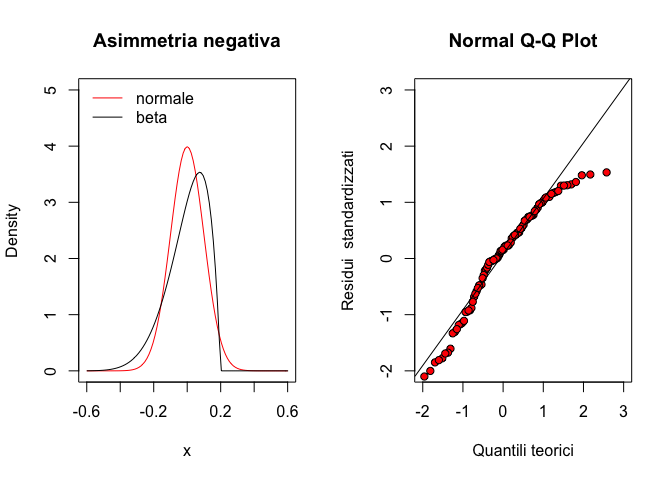
\includegraphics{_seedGerminationTutorial_files/figure-latex/unnamed-chunk-68-1.pdf}

\begin{Shaded}
\begin{Highlighting}[]
\FunctionTok{coeftest}\NormalTok{(modPmax, }\AttributeTok{vcov. =}\NormalTok{ sandwich)}
\DocumentationTok{\#\# }
\DocumentationTok{\#\# t test of coefficients:}
\DocumentationTok{\#\# }
\DocumentationTok{\#\#                     Estimate Std. Error   t value  Pr(\textgreater{}|t|)    }
\DocumentationTok{\#\# G:(Intercept)      1.0737381  0.0746708   14.3796 2.608e{-}11 ***}
\DocumentationTok{\#\# Psib:(Intercept)  {-}1.0053956  0.0016495 {-}609.5109 \textless{} 2.2e{-}16 ***}
\DocumentationTok{\#\# sigma:(Intercept)  0.1367469  0.0272873    5.0114 9.058e{-}05 ***}
\DocumentationTok{\#\# {-}{-}{-}}
\DocumentationTok{\#\# Signif. codes:  0 \textquotesingle{}***\textquotesingle{} 0.001 \textquotesingle{}**\textquotesingle{} 0.01 \textquotesingle{}*\textquotesingle{} 0.05 \textquotesingle{}.\textquotesingle{} 0.1 \textquotesingle{} \textquotesingle{} 1}
\end{Highlighting}
\end{Shaded}

Regarding the germination percentiles, a look at the data shows that, for all percentiles, germination rates stay constant up to -1 MPa and, afterwords, they increase linearly. We can model this behaviour by using the \texttt{GRPsiLin()} equation and, following Bradford (2002), we code a common base water potential level for the different germination percentiles. The code is given in the box below.

\begin{Shaded}
\begin{Highlighting}[]
\NormalTok{modGR }\OtherTok{\textless{}{-}} \FunctionTok{drm}\NormalTok{(Estimate }\SpecialCharTok{\textasciitilde{}}\NormalTok{ Psi, }\AttributeTok{data =}\NormalTok{ GRlist,}
               \AttributeTok{fct =} \FunctionTok{GRPsi.Lin}\NormalTok{(), }\AttributeTok{curveid =}\NormalTok{ g,}
             \AttributeTok{pmodels =} \FunctionTok{list}\NormalTok{(}\SpecialCharTok{\textasciitilde{}}\DecValTok{1}\NormalTok{, }\SpecialCharTok{\textasciitilde{}}\NormalTok{g }\SpecialCharTok{{-}} \DecValTok{1}\NormalTok{))}
\FunctionTok{plot}\NormalTok{(modGR, }\AttributeTok{log =} \StringTok{""}\NormalTok{,}
             \AttributeTok{legendPos =} \FunctionTok{c}\NormalTok{(}\SpecialCharTok{{-}}\FloatTok{1.3}\NormalTok{, }\FloatTok{0.7}\NormalTok{))}
\end{Highlighting}
\end{Shaded}

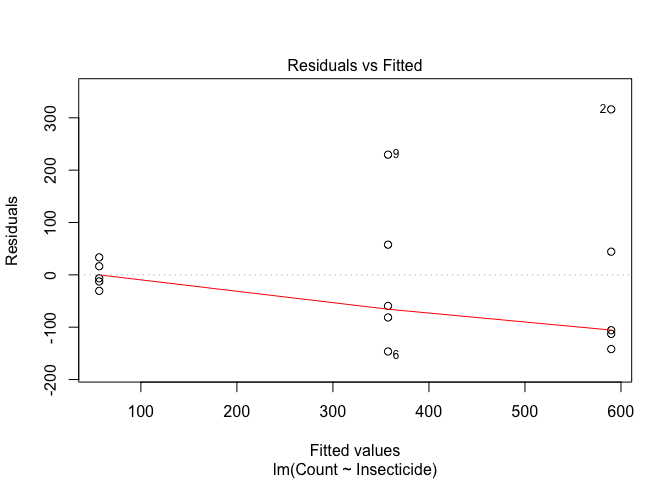
\includegraphics{_seedGerminationTutorial_files/figure-latex/unnamed-chunk-69-1.pdf}

\begin{Shaded}
\begin{Highlighting}[]
\FunctionTok{coeftest}\NormalTok{(modGR, }\AttributeTok{vcov. =}\NormalTok{ sandwich)}
\DocumentationTok{\#\# }
\DocumentationTok{\#\# t test of coefficients:}
\DocumentationTok{\#\# }
\DocumentationTok{\#\#                   Estimate Std. Error  t value  Pr(\textgreater{}|t|)    }
\DocumentationTok{\#\# Psib:(Intercept) {-}0.989504   0.031937 {-}30.9832 \textless{} 2.2e{-}16 ***}
\DocumentationTok{\#\# thetaH:g10\%       0.446550   0.081366   5.4881 8.977e{-}07 ***}
\DocumentationTok{\#\# thetaH:g30\%       0.649827   0.099213   6.5498 1.557e{-}08 ***}
\DocumentationTok{\#\# thetaH:g50\%       0.852974   0.134058   6.3627 3.209e{-}08 ***}
\DocumentationTok{\#\# {-}{-}{-}}
\DocumentationTok{\#\# Signif. codes:  0 \textquotesingle{}***\textquotesingle{} 0.001 \textquotesingle{}**\textquotesingle{} 0.01 \textquotesingle{}*\textquotesingle{} 0.05 \textquotesingle{}.\textquotesingle{} 0.1 \textquotesingle{} \textquotesingle{} 1}
\end{Highlighting}
\end{Shaded}

Usually, we are interested in the base osmotic potential level (\(\Psi_b\)) that is given in the output of the \texttt{coeftest()} method. We used \texttt{coeftest()} in the \texttt{lmtest} package for reasons that will be clearer later on.

\hypertarget{example-2}{%
\subsection{Example 2}\label{example-2}}

This second dataset was obtained from a germination assays with barley, where three replicates of 50 seeds were placed in Petri dishes and assayed at 9 constant temperature levels (1, 3, 7, 10, 15, 20, 25, 30, 35, 40 °C). Germinated seeds were counted and removed daily for 10 days. We have already presented this analysis in a previous paper (Onofri et al., 2018), although in this post we use a different (and updated) coding.

Also in this second example, the first step of data analysis is based on loading the data and fitting a separate time-to-event curve to the data at each temperature level.

\begin{Shaded}
\begin{Highlighting}[]
\FunctionTok{data}\NormalTok{(barley)}
\NormalTok{barley }\OtherTok{\textless{}{-}}\NormalTok{ barley }\SpecialCharTok{\%\textgreater{}\%} 
  \FunctionTok{mutate}\NormalTok{(}\AttributeTok{TempF =} \FunctionTok{factor}\NormalTok{(Temp))}

\NormalTok{mod1 }\OtherTok{\textless{}{-}} \FunctionTok{drmte}\NormalTok{(nSeeds }\SpecialCharTok{\textasciitilde{}}\NormalTok{ timeBef }\SpecialCharTok{+}\NormalTok{ timeAf, }\AttributeTok{fct=}\FunctionTok{W2.3}\NormalTok{(),}
      \AttributeTok{curveid =}\NormalTok{ TempF,}
      \AttributeTok{data =}\NormalTok{ barley,}
      \AttributeTok{separate =}\NormalTok{ T)}
\end{Highlighting}
\end{Shaded}

Now, we retrieve the germination rates for the 10\^{}th, 30\textsuperscript{th} and 50\textsuperscript{th} percentile; for analogy with the published paper, we restrict the percentiles to the germinated fraction, althoug it might be better to avoid such a restriction.

\begin{Shaded}
\begin{Highlighting}[]
\NormalTok{GR }\OtherTok{\textless{}{-}} \FunctionTok{quantile}\NormalTok{(mod1, }\AttributeTok{rate =}\NormalTok{ T, }\AttributeTok{restricted =}\NormalTok{ T, }
               \AttributeTok{probs =} \FunctionTok{c}\NormalTok{(}\FloatTok{0.1}\NormalTok{, }\FloatTok{0.3}\NormalTok{, }\FloatTok{0.5}\NormalTok{),}
                \AttributeTok{display =}\NormalTok{ F)}
\NormalTok{GRlist }\OtherTok{\textless{}{-}} \FunctionTok{tibble}\NormalTok{(}\AttributeTok{temp =} \FunctionTok{row.names}\NormalTok{(GR), GR, }\AttributeTok{row.names =} \ConstantTok{NULL}\NormalTok{) }\SpecialCharTok{\%\textgreater{}\%} 
  \FunctionTok{separate}\NormalTok{(}\AttributeTok{col =} \StringTok{"temp"}\NormalTok{, }\AttributeTok{into =} \FunctionTok{c}\NormalTok{(}\StringTok{"Temp"}\NormalTok{, }\StringTok{"g"}\NormalTok{),}
           \AttributeTok{sep =} \StringTok{":"}\NormalTok{) }\SpecialCharTok{\%\textgreater{}\%} 
  \FunctionTok{mutate}\NormalTok{(}\AttributeTok{Temp =} \FunctionTok{as.numeric}\NormalTok{(Temp)) }\SpecialCharTok{\%\textgreater{}\%} 
  \FunctionTok{remove\_rownames}\NormalTok{()}
\FunctionTok{head}\NormalTok{(GRlist)}
\DocumentationTok{\#\# \# A tibble: 6 x 4}
\DocumentationTok{\#\#    Temp g     Estimate      SE}
\DocumentationTok{\#\#   \textless{}dbl\textgreater{} \textless{}chr\textgreater{}    \textless{}dbl\textgreater{}   \textless{}dbl\textgreater{}}
\DocumentationTok{\#\# 1     1 10\%     0.0982 0.00328}
\DocumentationTok{\#\# 2     1 30\%     0.0777 0.00177}
\DocumentationTok{\#\# 3     1 50\%     0.0682 0.00125}
\DocumentationTok{\#\# 4     3 10\%     0.124  0.00307}
\DocumentationTok{\#\# 5     3 30\%     0.105  0.00173}
\DocumentationTok{\#\# 6     3 50\%     0.0962 0.00126}
\end{Highlighting}
\end{Shaded}

The behaviour of germination rates against temperature can be described, e.g., by using the threshold model proposed by Masin et al.~(2017), that is implemented in the R function \texttt{GRT.Ex()}, as shown in the box below. Preliminary trials show that the three percentiles share the same `k' parameter and base temperature level, which we can request by using the `pmodels' argument.

\begin{Shaded}
\begin{Highlighting}[]
\NormalTok{modGR }\OtherTok{\textless{}{-}} \FunctionTok{drm}\NormalTok{(Estimate }\SpecialCharTok{\textasciitilde{}}\NormalTok{ Temp, }\AttributeTok{data =}\NormalTok{ GRlist,}
               \AttributeTok{fct =} \FunctionTok{GRT.Ex}\NormalTok{(),}
             \AttributeTok{curveid =}\NormalTok{ g, }\AttributeTok{pmodels =} \FunctionTok{list}\NormalTok{(}\SpecialCharTok{\textasciitilde{}}\DecValTok{1}\NormalTok{, }\SpecialCharTok{\textasciitilde{}}\DecValTok{1}\NormalTok{, }\SpecialCharTok{\textasciitilde{}}\NormalTok{g }\SpecialCharTok{{-}} \DecValTok{1}\NormalTok{, }\SpecialCharTok{\textasciitilde{}}\NormalTok{g }\SpecialCharTok{{-}}\DecValTok{1}\NormalTok{))}
\FunctionTok{coeftest}\NormalTok{(modGR, }\AttributeTok{vcov. =}\NormalTok{ sandwich)}
\DocumentationTok{\#\# }
\DocumentationTok{\#\# t test of coefficients:}
\DocumentationTok{\#\# }
\DocumentationTok{\#\#                 Estimate Std. Error   t value  Pr(\textgreater{}|t|)    }
\DocumentationTok{\#\# k:(Intercept)   0.876849   0.138731    6.3205 4.577e{-}06 ***}
\DocumentationTok{\#\# Tb:(Intercept) {-}0.553318   0.774412   {-}0.7145    0.4836    }
\DocumentationTok{\#\# Tc:g10\%        35.200942   0.021761 1617.5850 \textless{} 2.2e{-}16 ***}
\DocumentationTok{\#\# Tc:g30\%        33.235421   0.321386  103.4129 \textless{} 2.2e{-}16 ***}
\DocumentationTok{\#\# Tc:g50\%        32.198489   0.225161  143.0021 \textless{} 2.2e{-}16 ***}
\DocumentationTok{\#\# ThetaT:g10\%    25.454497   1.788195   14.2347 1.378e{-}11 ***}
\DocumentationTok{\#\# ThetaT:g30\%    40.458899   2.001762   20.2116 2.630e{-}14 ***}
\DocumentationTok{\#\# ThetaT:g50\%    51.413920   2.415663   21.2836 1.025e{-}14 ***}
\DocumentationTok{\#\# {-}{-}{-}}
\DocumentationTok{\#\# Signif. codes:  0 \textquotesingle{}***\textquotesingle{} 0.001 \textquotesingle{}**\textquotesingle{} 0.01 \textquotesingle{}*\textquotesingle{} 0.05 \textquotesingle{}.\textquotesingle{} 0.1 \textquotesingle{} \textquotesingle{} 1}
\FunctionTok{plot}\NormalTok{(modGR, }\AttributeTok{log =} \StringTok{""}\NormalTok{, }\AttributeTok{type =} \StringTok{"all"}\NormalTok{, }\AttributeTok{xlim =} \FunctionTok{c}\NormalTok{(}\DecValTok{0}\NormalTok{, }\DecValTok{40}\NormalTok{),}
     \AttributeTok{ylim =} \FunctionTok{c}\NormalTok{(}\DecValTok{0}\NormalTok{, }\FloatTok{1.3}\NormalTok{),}
     \AttributeTok{ylab =} \StringTok{"GR"}\NormalTok{, }\AttributeTok{xlab =} \StringTok{"Temperature (°C)"}\NormalTok{,}
     \AttributeTok{legendPos =} \FunctionTok{c}\NormalTok{(}\DecValTok{12}\NormalTok{, }\FloatTok{0.9}\NormalTok{))}
\end{Highlighting}
\end{Shaded}

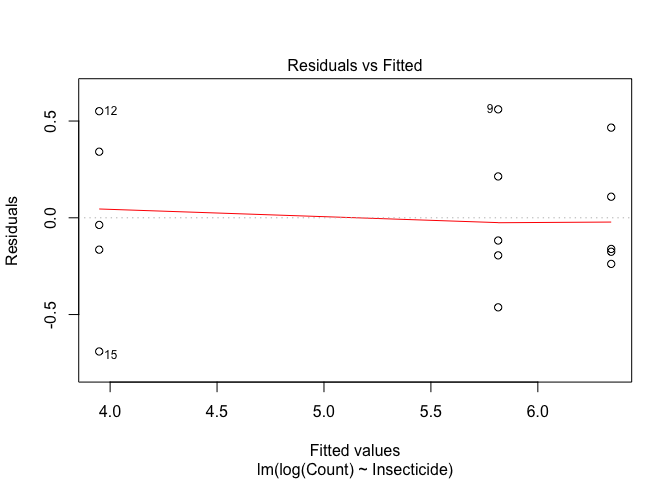
\includegraphics{_seedGerminationTutorial_files/figure-latex/unnamed-chunk-72-1.pdf}

\hypertarget{warning-message}{%
\subsection{Warning message!}\label{warning-message}}

When we collect data about the response of germination rates to temperature and use them to parameterise nonlinear regression models by using nonlinear least squares, the basic assumption of homoscedasticity is rarely tenable. \textbf{We should not forget this!}. In the above examples I used a robust variance-covariance sandwich estimator (Zeileis, 2006; see the use of the \texttt{coeftest()} method, instead of the \texttt{summary()} method), although other techniques can be successfully used to deal with this problem.

\hypertarget{carrying-over-information-to-the-2nd-step}{%
\section{\texorpdfstring{Carrying over information to the 2\textsuperscript{nd} step}{Carrying over information to the 2nd step}}\label{carrying-over-information-to-the-2nd-step}}

(yet to be done)

\hypertarget{examples-and-case-studies}{%
\chapter{Examples and case-studies}\label{examples-and-case-studies}}

\hypertarget{fitting-hydro-thermal-time-models-to-seed-germination-data}{%
\section{Fitting hydro-thermal-time-models to seed germination data}\label{fitting-hydro-thermal-time-models-to-seed-germination-data}}

This dataset was obtained from previously published work (Mesgaran et al., 2017) with \emph{Hordeum spontaneum} {[}C. Koch{]} Thell. The germination assay was conducted using four replicates of 20 seeds tested at six different water potential levels (0, −0.3, −0.6, −0.9, −1.2 and −1.5 MPa). Osmotic potentials were produced using variable amount of polyethylene glycol (PEG, molecular weight 8000) adjusted for the temperature level. Petri dishes were incubated at six constant temperature levels (8, 12, 16, 20, 24 and 28 °C), under a photoperiod of 12 h. Germinated seeds (radicle protrusion \textgreater{} 3 mm) were counted and removed daily for 20 days.

This dataset is available as \texttt{hordeum} in the \texttt{drcSeedGerm} package, which needs to be installed from github (see below), together the package \texttt{drcte}, which is necessary to fit time-to-event models. The following code loads the necessary packages, loads the dataset \texttt{rape} and shows the first six lines.

\begin{Shaded}
\begin{Highlighting}[]
\CommentTok{\# Installing packages (only at first instance)}
\CommentTok{\# library(devtools)}
\CommentTok{\# install\_github("OnofriAndreaPG/drcSeedGerm")}
\CommentTok{\# install\_github("OnofriAndreaPG/drcte")}
\FunctionTok{library}\NormalTok{(drcSeedGerm)}
\FunctionTok{library}\NormalTok{(tidyverse)}
\FunctionTok{data}\NormalTok{(hordeum)}
\FunctionTok{head}\NormalTok{(hordeum)}
\DocumentationTok{\#\#   temp water Dish timeBef timeAf nViable nSeeds nCum}
\DocumentationTok{\#\# 1    8  {-}1.5    1       0     24      20      0    0}
\DocumentationTok{\#\# 2    8  {-}1.5    1      24     48      20      0    0}
\DocumentationTok{\#\# 3    8  {-}1.5    1      48     72      20      0    0}
\DocumentationTok{\#\# 4    8  {-}1.5    1      72     96      20      0    0}
\DocumentationTok{\#\# 5    8  {-}1.5    1      96    120      20      0    0}
\DocumentationTok{\#\# 6    8  {-}1.5    1     120    144      20      1    1}
\end{Highlighting}
\end{Shaded}

\hypertarget{preliminary-analyses}{%
\subsection{Preliminary analyses}\label{preliminary-analyses}}

First of all, it is necessary to mention that \textbf{this dataset was already analysed in Onofri et al.~(2018; Example 2) by using the same methodology, although, in that paper, the R implementation was different (see Supplemental Material) and it is now outdated.}

In the above data frame, `timeAf' represents the moment when germinated seeds were counted, while 'timeBef' represents the previous inspection time (or the beginning of the assay). The column 'nSeeds' is the number of seeds that germinated during the time interval between `timeBef' and `timeAf. The 'nCum' column contains the cumulative number of germinated seeds and it is not necessary for time-to-event model fitting, although we can use it for plotting purposes.

\begin{Shaded}
\begin{Highlighting}[]
\NormalTok{hordeum }\OtherTok{\textless{}{-}}\NormalTok{ hordeum }\SpecialCharTok{\%\textgreater{}\%} 
  \FunctionTok{mutate}\NormalTok{(}\AttributeTok{propCum =}\NormalTok{ nCum}\SpecialCharTok{/}\NormalTok{nViable)}

\FunctionTok{ggplot}\NormalTok{(}\AttributeTok{data =}\NormalTok{ hordeum, }\AttributeTok{mapping =} \FunctionTok{aes}\NormalTok{(timeAf, propCum)) }\SpecialCharTok{+}
  \FunctionTok{geom\_point}\NormalTok{() }\SpecialCharTok{+}
  \FunctionTok{facet\_grid}\NormalTok{(temp }\SpecialCharTok{\textasciitilde{}}\NormalTok{ water) }\SpecialCharTok{+}
  \FunctionTok{scale\_x\_continuous}\NormalTok{(}\AttributeTok{name =} \StringTok{"Time (d)"}\NormalTok{) }\SpecialCharTok{+}
  \FunctionTok{scale\_y\_continuous}\NormalTok{(}\AttributeTok{name =} \StringTok{"Cumulative proportion of germinated seeds"}\NormalTok{)}
\end{Highlighting}
\end{Shaded}

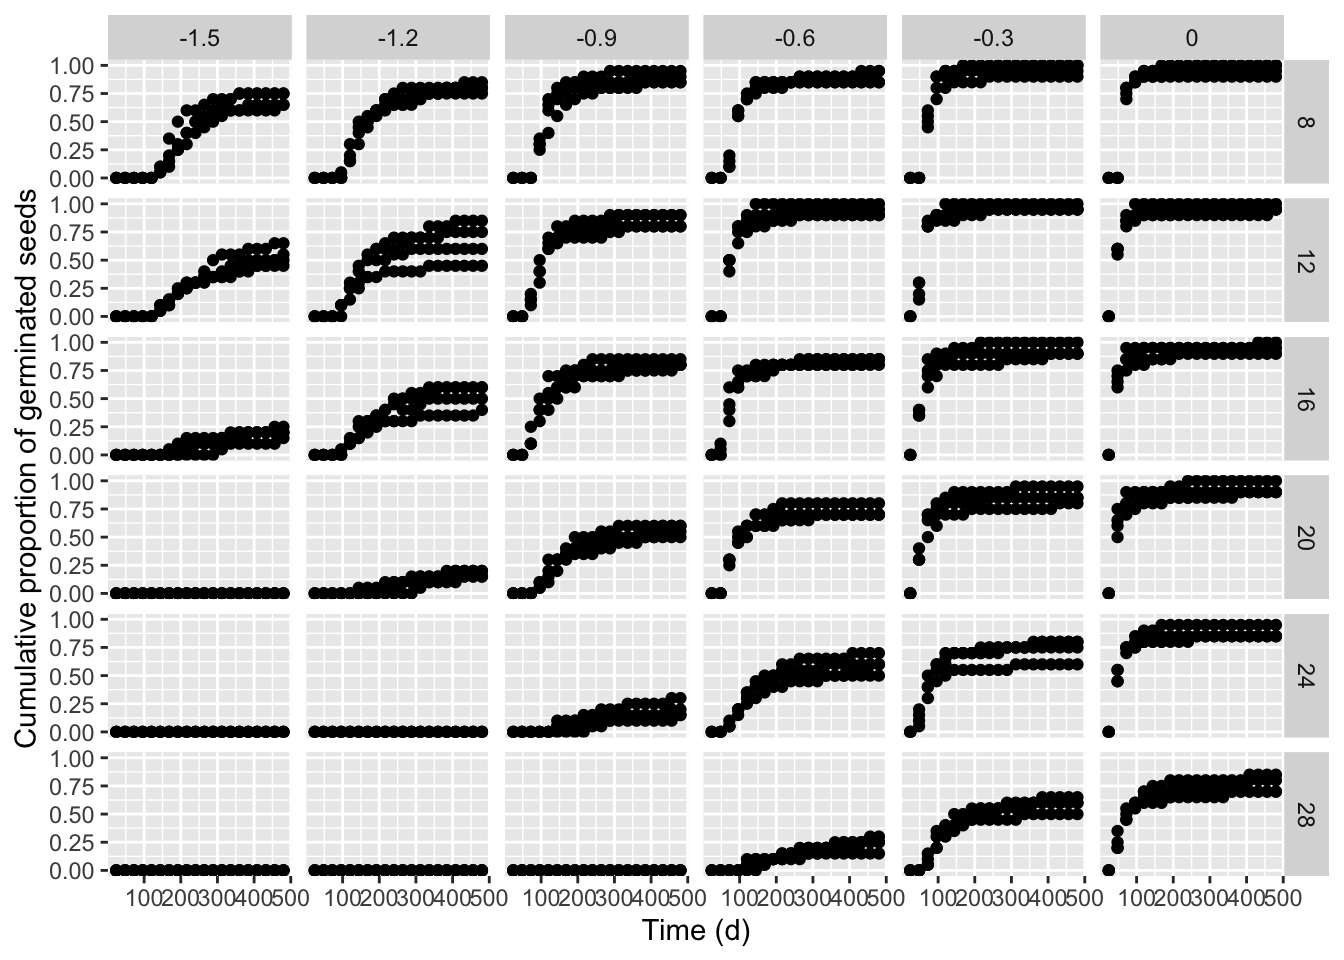
\includegraphics{_seedGerminationTutorial_files/figure-latex/unnamed-chunk-74-1.pdf}

We see that the germination time-course is strongly affected by both temperature and water potential in the substrate and, consequently, our obvious interest is to model the effects of those environmental covariates. In our manuscript, we started from the idea that a parametric time-to-event curve is defined as a cumulative probability function (\(\Phi\)), with three parameters:

\[P(t) = \Phi \left( b, d, e \right)\]
where \(P(t)\) is the cumulative probability of germination at time \(t\), \(e\) is the median germination time, \(b\) is the slope at the inflection point and \(d\) is the maximum germinated proportion. The most obvious extension is to allow for different \(b\), \(d\) and \(e\) values for each of the i\textsuperscript{th} combinations of water potential (\(\Psi\)) and temperature level (\(T\)):

\[P(t, \Psi, T) = \Phi \left( b_i, d_i, e_i \right)\]
From the graph above, we see several `degenerated' time-to-event curves, where no germinations occurred (e.g., see the graph at -1.5 MPa and 28°C). In order to avoid problems with those curves, we can use the \texttt{drmte()} function and set the \texttt{separate\ =\ TRUE} argument, so that the different curves are fitted independently of one another and the degenerated curves are recognised and skipped, without stopping the execution in R. In particular, where no time-course of events can be estimated, it is assumed that there is no progress to germination during the study-period and that the cumulative proportion of germinated seeds remains constant across that period. Consequently, the \texttt{drmte()} function resorts to fitting a simpler model, where the only \(d\) parameter is estimated (that is the maximum fraction of germinated seeds).

\begin{Shaded}
\begin{Highlighting}[]
\NormalTok{hordeum }\OtherTok{\textless{}{-}}\NormalTok{ hordeum }\SpecialCharTok{\%\textgreater{}\%} 
  \FunctionTok{mutate}\NormalTok{(}\AttributeTok{comb =} \FunctionTok{factor}\NormalTok{( }\FunctionTok{factor}\NormalTok{(water)}\SpecialCharTok{:}\FunctionTok{factor}\NormalTok{(temp)))}
\NormalTok{mod1 }\OtherTok{\textless{}{-}} \FunctionTok{drmte}\NormalTok{(nSeeds }\SpecialCharTok{\textasciitilde{}}\NormalTok{ timeBef }\SpecialCharTok{+}\NormalTok{ timeAf, }\AttributeTok{data =}\NormalTok{ hordeum,}
             \AttributeTok{curveid =}\NormalTok{ comb, }\AttributeTok{fct =} \FunctionTok{loglogistic}\NormalTok{(),}
             \AttributeTok{separate =} \ConstantTok{TRUE}\NormalTok{)}
\FunctionTok{summary}\NormalTok{(mod1)}
\DocumentationTok{\#\# }
\DocumentationTok{\#\# Model fitted: Separate fitting of several time{-}to{-}event curves}
\DocumentationTok{\#\# }
\DocumentationTok{\#\# Robust estimation: no }
\DocumentationTok{\#\# }
\DocumentationTok{\#\# Parameter estimates:}
\DocumentationTok{\#\# }
\DocumentationTok{\#\#             Estimate Std. Error t{-}value   p{-}value    }
\DocumentationTok{\#\# b:{-}1.5:8    5.577670   0.671086  8.3114 \textless{} 2.2e{-}16 ***}
\DocumentationTok{\#\# d:{-}1.5:8    0.705845   0.051801 13.6260 \textless{} 2.2e{-}16 ***}
\DocumentationTok{\#\# e:{-}1.5:8  203.532986   8.746552 23.2701 \textless{} 2.2e{-}16 ***}
\DocumentationTok{\#\# b:{-}1.5:12   4.036639   0.633750  6.3694 1.897e{-}10 ***}
\DocumentationTok{\#\# d:{-}1.5:12   0.566163   0.061406  9.2201 \textless{} 2.2e{-}16 ***}
\DocumentationTok{\#\# e:{-}1.5:12 232.198040  17.347102 13.3854 \textless{} 2.2e{-}16 ***}
\DocumentationTok{\#\# b:{-}1.5:16   4.130712   1.174395  3.5173 0.0004359 ***}
\DocumentationTok{\#\# d:{-}1.5:16   0.226248   0.057013  3.9683 7.238e{-}05 ***}
\DocumentationTok{\#\# e:{-}1.5:16 293.584384  41.294139  7.1096 1.164e{-}12 ***}
\DocumentationTok{\#\# d:{-}1.5:20   0.000000   0.000000     NaN       NaN    }
\DocumentationTok{\#\# d:{-}1.5:24   0.000000   0.000000     NaN       NaN    }
\DocumentationTok{\#\# d:{-}1.5:28   0.000000   0.000000     NaN       NaN    }
\DocumentationTok{\#\# b:{-}1.2:8    4.761454   0.531157  8.9643 \textless{} 2.2e{-}16 ***}
\DocumentationTok{\#\# d:{-}1.2:8    0.803436   0.044972 17.8653 \textless{} 2.2e{-}16 ***}
\DocumentationTok{\#\# e:{-}1.2:8  152.794391   7.123662 21.4489 \textless{} 2.2e{-}16 ***}
\DocumentationTok{\#\# b:{-}1.2:12   4.165847   0.518344  8.0368 9.050e{-}16 ***}
\DocumentationTok{\#\# d:{-}1.2:12   0.667099   0.053329 12.5092 \textless{} 2.2e{-}16 ***}
\DocumentationTok{\#\# e:{-}1.2:12 145.571114   8.562685 17.0006 \textless{} 2.2e{-}16 ***}
\DocumentationTok{\#\# b:{-}1.2:16   3.848053   0.556564  6.9140 4.713e{-}12 ***}
\DocumentationTok{\#\# d:{-}1.2:16   0.536017   0.057474  9.3262 \textless{} 2.2e{-}16 ***}
\DocumentationTok{\#\# e:{-}1.2:16 175.692653  13.009048 13.5054 \textless{} 2.2e{-}16 ***}
\DocumentationTok{\#\# b:{-}1.2:20   4.679284   1.377885  3.3960 0.0006838 ***}
\DocumentationTok{\#\# d:{-}1.2:20   0.191881   0.049814  3.8520 0.0001172 ***}
\DocumentationTok{\#\# e:{-}1.2:20 291.173467  34.870683  8.3501 \textless{} 2.2e{-}16 ***}
\DocumentationTok{\#\# d:{-}1.2:24   0.000000   0.000000     NaN       NaN    }
\DocumentationTok{\#\# d:{-}1.2:28   0.000000   0.000000     NaN       NaN    }
\DocumentationTok{\#\# b:{-}0.9:8    5.237479   0.550871  9.5076 \textless{} 2.2e{-}16 ***}
\DocumentationTok{\#\# d:{-}0.9:8    0.887920   0.035345 25.1218 \textless{} 2.2e{-}16 ***}
\DocumentationTok{\#\# e:{-}0.9:8  111.384281   4.427060 25.1599 \textless{} 2.2e{-}16 ***}
\DocumentationTok{\#\# b:{-}0.9:12   4.368990   0.475050  9.1969 \textless{} 2.2e{-}16 ***}
\DocumentationTok{\#\# d:{-}0.9:12   0.850876   0.039968 21.2889 \textless{} 2.2e{-}16 ***}
\DocumentationTok{\#\# e:{-}0.9:12  99.501087   4.833892 20.5841 \textless{} 2.2e{-}16 ***}
\DocumentationTok{\#\# b:{-}0.9:16   3.581796   0.400722  8.9383 \textless{} 2.2e{-}16 ***}
\DocumentationTok{\#\# d:{-}0.9:16   0.816041   0.043892 18.5922 \textless{} 2.2e{-}16 ***}
\DocumentationTok{\#\# e:{-}0.9:16 105.233306   6.461986 16.2850 \textless{} 2.2e{-}16 ***}
\DocumentationTok{\#\# b:{-}0.9:20   3.536663   0.502112  7.0436 1.874e{-}12 ***}
\DocumentationTok{\#\# d:{-}0.9:20   0.572734   0.056895 10.0665 \textless{} 2.2e{-}16 ***}
\DocumentationTok{\#\# e:{-}0.9:20 154.543645  11.924187 12.9605 \textless{} 2.2e{-}16 ***}
\DocumentationTok{\#\# b:{-}0.9:24   3.113060   0.947598  3.2852 0.0010191 ** }
\DocumentationTok{\#\# d:{-}0.9:24   0.233165   0.062870  3.7087 0.0002084 ***}
\DocumentationTok{\#\# e:{-}0.9:24 269.509412  55.515112  4.8547 1.206e{-}06 ***}
\DocumentationTok{\#\# d:{-}0.9:28   0.000000   0.000000     NaN       NaN    }
\DocumentationTok{\#\# b:{-}0.6:8    5.077994   0.538321  9.4330 \textless{} 2.2e{-}16 ***}
\DocumentationTok{\#\# d:{-}0.6:8    0.900202   0.033548 26.8334 \textless{} 2.2e{-}16 ***}
\DocumentationTok{\#\# e:{-}0.6:8   92.146203   3.725399 24.7346 \textless{} 2.2e{-}16 ***}
\DocumentationTok{\#\# b:{-}0.6:12   5.564019   0.586966  9.4793 \textless{} 2.2e{-}16 ***}
\DocumentationTok{\#\# d:{-}0.6:12   0.937528   0.027059 34.6476 \textless{} 2.2e{-}16 ***}
\DocumentationTok{\#\# e:{-}0.6:12  74.982399   2.818636 26.6024 \textless{} 2.2e{-}16 ***}
\DocumentationTok{\#\# b:{-}0.6:16   4.144136   0.458813  9.0323 \textless{} 2.2e{-}16 ***}
\DocumentationTok{\#\# d:{-}0.6:16   0.837853   0.041271 20.3014 \textless{} 2.2e{-}16 ***}
\DocumentationTok{\#\# e:{-}0.6:16  75.109147   3.897277 19.2722 \textless{} 2.2e{-}16 ***}
\DocumentationTok{\#\# b:{-}0.6:20   4.399408   0.510297  8.6213 \textless{} 2.2e{-}16 ***}
\DocumentationTok{\#\# d:{-}0.6:20   0.725331   0.049946 14.5224 \textless{} 2.2e{-}16 ***}
\DocumentationTok{\#\# e:{-}0.6:20  83.735884   4.468212 18.7404 \textless{} 2.2e{-}16 ***}
\DocumentationTok{\#\# b:{-}0.6:24   3.269465   0.443121  7.3783 1.603e{-}13 ***}
\DocumentationTok{\#\# d:{-}0.6:24   0.607528   0.055700 10.9071 \textless{} 2.2e{-}16 ***}
\DocumentationTok{\#\# e:{-}0.6:24 125.859897   9.985513 12.6042 \textless{} 2.2e{-}16 ***}
\DocumentationTok{\#\# b:{-}0.6:28   2.959772   0.767672  3.8555 0.0001155 ***}
\DocumentationTok{\#\# d:{-}0.6:28   0.265633   0.059199  4.4871 7.220e{-}06 ***}
\DocumentationTok{\#\# e:{-}0.6:28 233.440197  40.981613  5.6962 1.225e{-}08 ***}
\DocumentationTok{\#\# b:{-}0.3:8    6.489283   0.700089  9.2692 \textless{} 2.2e{-}16 ***}
\DocumentationTok{\#\# d:{-}0.3:8    0.962474   0.021243 45.3069 \textless{} 2.2e{-}16 ***}
\DocumentationTok{\#\# e:{-}0.3:8   72.248403   2.326579 31.0535 \textless{} 2.2e{-}16 ***}
\DocumentationTok{\#\# b:{-}0.3:12   5.571444   0.614984  9.0595 \textless{} 2.2e{-}16 ***}
\DocumentationTok{\#\# d:{-}0.3:12   0.962476   0.021243 45.3075 \textless{} 2.2e{-}16 ***}
\DocumentationTok{\#\# e:{-}0.3:12  56.804335   2.154440 26.3662 \textless{} 2.2e{-}16 ***}
\DocumentationTok{\#\# b:{-}0.3:16   3.759741   0.406837  9.2414 \textless{} 2.2e{-}16 ***}
\DocumentationTok{\#\# d:{-}0.3:16   0.925252   0.029452 31.4157 \textless{} 2.2e{-}16 ***}
\DocumentationTok{\#\# e:{-}0.3:16  53.997403   3.004606 17.9715 \textless{} 2.2e{-}16 ***}
\DocumentationTok{\#\# b:{-}0.3:20   3.455788   0.382078  9.0447 \textless{} 2.2e{-}16 ***}
\DocumentationTok{\#\# d:{-}0.3:20   0.863032   0.038527 22.4004 \textless{} 2.2e{-}16 ***}
\DocumentationTok{\#\# e:{-}0.3:20  56.589306   3.525940 16.0494 \textless{} 2.2e{-}16 ***}
\DocumentationTok{\#\# b:{-}0.3:24   3.219012   0.384905  8.3631 \textless{} 2.2e{-}16 ***}
\DocumentationTok{\#\# d:{-}0.3:24   0.739176   0.049321 14.9869 \textless{} 2.2e{-}16 ***}
\DocumentationTok{\#\# e:{-}0.3:24  72.448658   5.145402 14.0803 \textless{} 2.2e{-}16 ***}
\DocumentationTok{\#\# b:{-}0.3:28   3.384884   0.449578  7.5290 5.110e{-}14 ***}
\DocumentationTok{\#\# d:{-}0.3:28   0.591722   0.055517 10.6583 \textless{} 2.2e{-}16 ***}
\DocumentationTok{\#\# e:{-}0.3:28 111.482975   8.597283 12.9672 \textless{} 2.2e{-}16 ***}
\DocumentationTok{\#\# b:0:8       8.055166   0.890908  9.0415 \textless{} 2.2e{-}16 ***}
\DocumentationTok{\#\# d:0:8       0.962496   0.021229 45.3391 \textless{} 2.2e{-}16 ***}
\DocumentationTok{\#\# e:0:8      64.579539   1.810276 35.6739 \textless{} 2.2e{-}16 ***}
\DocumentationTok{\#\# b:0:12      4.597148   0.515642  8.9154 \textless{} 2.2e{-}16 ***}
\DocumentationTok{\#\# d:0:12      0.962502   0.021236 45.3239 \textless{} 2.2e{-}16 ***}
\DocumentationTok{\#\# e:0:12     45.258150   2.124034 21.3076 \textless{} 2.2e{-}16 ***}
\DocumentationTok{\#\# b:0:16      4.519281   0.504988  8.9493 \textless{} 2.2e{-}16 ***}
\DocumentationTok{\#\# d:0:16      0.937575   0.027033 34.6821 \textless{} 2.2e{-}16 ***}
\DocumentationTok{\#\# e:0:16     41.805944   2.052607 20.3672 \textless{} 2.2e{-}16 ***}
\DocumentationTok{\#\# b:0:20      3.833745   0.419743  9.1335 \textless{} 2.2e{-}16 ***}
\DocumentationTok{\#\# d:0:20      0.925095   0.029446 31.4163 \textless{} 2.2e{-}16 ***}
\DocumentationTok{\#\# e:0:20     43.588297   2.434550 17.9040 \textless{} 2.2e{-}16 ***}
\DocumentationTok{\#\# b:0:24      4.103341   0.467512  8.7770 \textless{} 2.2e{-}16 ***}
\DocumentationTok{\#\# d:0:24      0.875057   0.036978 23.6641 \textless{} 2.2e{-}16 ***}
\DocumentationTok{\#\# e:0:24     47.161280   2.550713 18.4894 \textless{} 2.2e{-}16 ***}
\DocumentationTok{\#\# b:0:28      2.895784   0.341099  8.4896 \textless{} 2.2e{-}16 ***}
\DocumentationTok{\#\# d:0:28      0.764633   0.047737 16.0176 \textless{} 2.2e{-}16 ***}
\DocumentationTok{\#\# e:0:28     63.034588   4.939641 12.7610 \textless{} 2.2e{-}16 ***}
\DocumentationTok{\#\# {-}{-}{-}}
\DocumentationTok{\#\# Signif. codes:  0 \textquotesingle{}***\textquotesingle{} 0.001 \textquotesingle{}**\textquotesingle{} 0.01 \textquotesingle{}*\textquotesingle{} 0.05 \textquotesingle{}.\textquotesingle{} 0.1 \textquotesingle{} \textquotesingle{} 1}
\end{Highlighting}
\end{Shaded}

\hypertarget{a-better-modelling-approach-1}{%
\subsection{A better modelling approach}\label{a-better-modelling-approach-1}}

The previous approach is clearly sub-optimal, as the temperature and water potential levels are regarded as factors, i.e.~as nominal classes with no intrinsic orderings and distances. It would be much better to recognise that temperature and water potential are continuous variables and, consequently, code a time-to-event model where the three parameters are expressed as continuous functions of \(\Psi\) and \(T\):

\[P(t, \Psi, T) = \Phi \left[ b(\Psi, T), d(\Psi, T), e(\Psi, T) \right]\]

In the above mentioned manuscript (Onofri et al., 2018; example 2) we used a log-logistic cumulative distribution function:

\[P(t, \Psi, T) = \frac{ d(\Psi, T) }{1 + \exp \left\{ b \left[ \log(t) - \log( e(\Psi, T) ) \right] \right\} }\]

Considering that the germination rate is the inverse of germination time, we replaced \(e(\Psi, T) = 1/GR_{50}(\Psi, T)\) and used the following sub-models:

\[d(\Psi, T) = \textrm{max} \left\{ G \, \left[ 1 - \exp \left( \frac{ \Psi - \Psi_b - k(T - T_b )}{\sigma_{\Psi_b}} \right) \right]; 0 \right\}\]

\[GR_{50}(\Psi, T) = \textrm{max} \left\{ \frac{T - T_b }{\theta_{HT}} \left[\Psi - \Psi_b - k(T - T_b )\right]; 0 \right\}\]
Please, note that the shape parameter \(b\) has been regarded as independent from the environmental covariates. It may be useful to note that the the parameters are:

\begin{enumerate}
\def\labelenumi{\arabic{enumi}.}
\tightlist
\item
  \(\Psi_{b}\), that is the median base water potential in the seed lot,
\item
  \(T_{b}\), that is the base temperature for germination,
\item
  \(\theta_HT\), that is the hydro-thermal-time parameter,
\item
  \(\sigma_{\Psi_b}\), that represents the variability of \(\Psi_b\) within the population,
\item
  \(G\), that is the germinable fraction, accounting for the fact that \(d\) may not reach 1, regardless of time and water potential.
\item
  \(k\) and \(b\) that are parameters of shape.
\end{enumerate}

You can get more information from our original paper (Onofri et al., 2018). This hydro-thermal-time model was implemented in R as the \texttt{HTTEM()} function, and it is available within the \texttt{drcSeedGerm} package; we can fit it by using the \texttt{drmte()} function in the \texttt{drcte} package, but we need to provide starting values for model parameters, because the self-starting routine is not yet available. Finally, the \texttt{summary()} method can be used to retrieve the parameter estimates.

\begin{Shaded}
\begin{Highlighting}[]
\CommentTok{\# Complex model and slow fitting}
\NormalTok{modHTTE }\OtherTok{\textless{}{-}} \FunctionTok{drmte}\NormalTok{(nSeeds }\SpecialCharTok{\textasciitilde{}}\NormalTok{ timeBef }\SpecialCharTok{+}\NormalTok{ timeAf }\SpecialCharTok{+}\NormalTok{ water }\SpecialCharTok{+}\NormalTok{ temp,}
                 \AttributeTok{data=}\NormalTok{hordeum,}
                 \AttributeTok{fct =} \FunctionTok{HTTEM}\NormalTok{(),}
  \AttributeTok{start=}\FunctionTok{c}\NormalTok{(}\FloatTok{0.8}\NormalTok{,}\SpecialCharTok{{-}}\DecValTok{2}\NormalTok{, }\FloatTok{0.05}\NormalTok{, }\DecValTok{3}\NormalTok{, }\FloatTok{0.2}\NormalTok{, }\DecValTok{2000}\NormalTok{, }\FloatTok{0.5}\NormalTok{))}
\FunctionTok{summary}\NormalTok{(modHTTE, }\AttributeTok{robust =}\NormalTok{ T, }\AttributeTok{units =}\NormalTok{ Dish)}
\DocumentationTok{\#\# }
\DocumentationTok{\#\# Model fitted: Hydro{-}thermal{-}time{-}model (Mesgaran et al., 2017)}
\DocumentationTok{\#\# }
\DocumentationTok{\#\# Robust estimation: Cluster robust sandwich SEs }
\DocumentationTok{\#\# }
\DocumentationTok{\#\# Parameter estimates:}
\DocumentationTok{\#\# }
\DocumentationTok{\#\#                          Estimate  Std. Error  t value Pr(\textgreater{}|t|)    }
\DocumentationTok{\#\# G:(Intercept)          9.8820e{-}01  1.1576e{-}02  85.3692   \textless{}2e{-}16 ***}
\DocumentationTok{\#\# Psib:(Intercept)      {-}2.9133e+00  3.4812e{-}02 {-}83.6874   \textless{}2e{-}16 ***}
\DocumentationTok{\#\# kt:(Intercept)         7.4228e{-}02  1.2666e{-}03  58.6015   \textless{}2e{-}16 ***}
\DocumentationTok{\#\# Tb:(Intercept)        {-}7.4525e{-}01  3.5254e{-}01  {-}2.1139   0.0346 *  }
\DocumentationTok{\#\# sigmaPsib:(Intercept)  5.5284e{-}01  2.8976e{-}02  19.0790   \textless{}2e{-}16 ***}
\DocumentationTok{\#\# ThetaHT:(Intercept)    1.3091e+03  4.0638e+01  32.2130   \textless{}2e{-}16 ***}
\DocumentationTok{\#\# b:(Intercept)          4.1650e+00  1.1332e{-}01  36.7548   \textless{}2e{-}16 ***}
\DocumentationTok{\#\# {-}{-}{-}}
\DocumentationTok{\#\# Signif. codes:  0 \textquotesingle{}***\textquotesingle{} 0.001 \textquotesingle{}**\textquotesingle{} 0.01 \textquotesingle{}*\textquotesingle{} 0.05 \textquotesingle{}.\textquotesingle{} 0.1 \textquotesingle{} \textquotesingle{} 1}
\end{Highlighting}
\end{Shaded}

It is always important not to neglect a graphical inspection of model fit. The \texttt{plot()} method does not work with time-to-event curves with additional covariates (apart from time). However, we can retrieve the fitted data by using the \texttt{plotData()} function and use those predictions within the \texttt{ggplot()} function. The box below shows the appropriate coding.

\begin{Shaded}
\begin{Highlighting}[]
\NormalTok{tab }\OtherTok{\textless{}{-}} \FunctionTok{plotData}\NormalTok{(modHTTE)}

\FunctionTok{ggplot}\NormalTok{() }\SpecialCharTok{+}
  \FunctionTok{geom\_point}\NormalTok{(}\AttributeTok{data =}\NormalTok{ tab}\SpecialCharTok{$}\NormalTok{plotPoints, }\AttributeTok{mapping =} \FunctionTok{aes}\NormalTok{(}\AttributeTok{x =}\NormalTok{ timeAf, }\AttributeTok{y =}\NormalTok{ CDF),}
            \AttributeTok{col =} \StringTok{"red"}\NormalTok{) }\SpecialCharTok{+}
  \FunctionTok{geom\_line}\NormalTok{(}\AttributeTok{data =}\NormalTok{ tab}\SpecialCharTok{$}\NormalTok{plotFits, }\AttributeTok{mapping =} \FunctionTok{aes}\NormalTok{(}\AttributeTok{x =}\NormalTok{ timeAf, }\AttributeTok{y =}\NormalTok{ CDF)) }\SpecialCharTok{+}
  \FunctionTok{facet\_grid}\NormalTok{(temp }\SpecialCharTok{\textasciitilde{}}\NormalTok{ water) }\SpecialCharTok{+}
  \FunctionTok{scale\_x\_continuous}\NormalTok{(}\AttributeTok{name =} \StringTok{"Time (d)"}\NormalTok{) }\SpecialCharTok{+}
  \FunctionTok{scale\_y\_continuous}\NormalTok{(}\AttributeTok{name =} \StringTok{"Cumulative proportion of germinated seeds"}\NormalTok{)}
\end{Highlighting}
\end{Shaded}

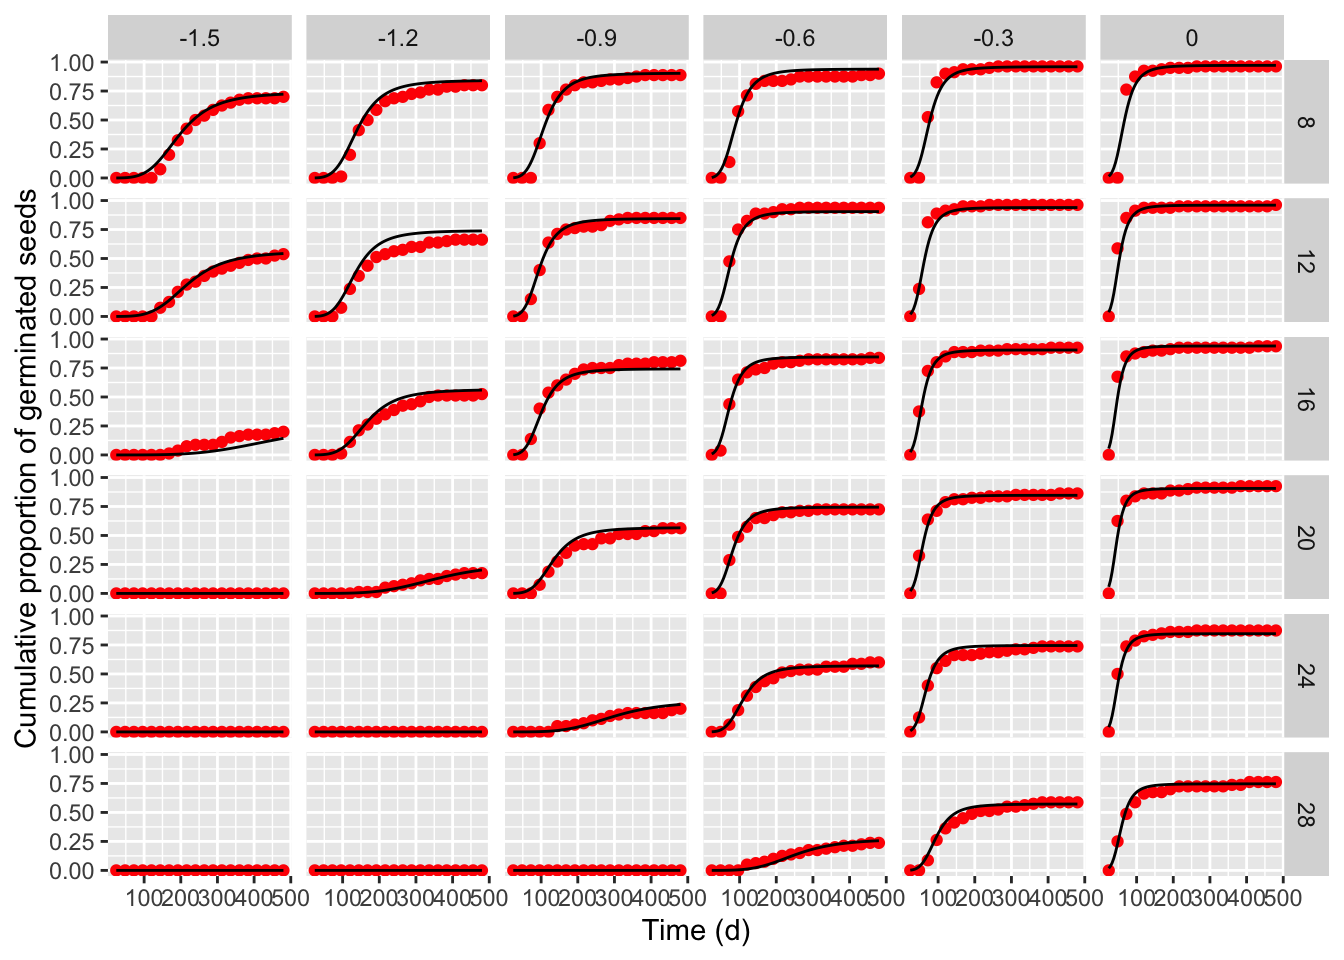
\includegraphics{_seedGerminationTutorial_files/figure-latex/unnamed-chunk-77-1.pdf}

\hypertarget{other-htt-models}{%
\subsection{Other HTT models}\label{other-htt-models}}

Mohsen Mesgaran, in an earlier paper (Mesgaran et al., 2017), used a different modelling approach, where he did not directly consider the distribution of germination times within the seed lot, but modelled the distribution of base water potential levels within the lot, under the idea that different germination times arise as the result of the fact that each seed has its `intrinsic' water potential level (Bradford, 1992). We do not give any further biological detail, because this is only meant to be a post about R coding; you can refer to Bradford (1992), Mesgaran et al.~(2013) and Mesgaran et al.~(2017) for this detail. The following equation describes the time-course of germination depending on temperature and water potential level, assuming that the distribution of base water potential in the seed lot is gaussian:

\[ P(t, T, \Psi) = \Phi \left\{ \frac{\Psi - \left[ \frac{\theta_{HT}}{t (T - T_b)} \right] - \left[\Psi_b + K_t (T - T_b) \right] }{\sigma_{\Psi_b}} \right\}   \quad \quad (\textrm{HTTnorm.M})\]

where \(P\) is the proportion of germinated seeds, depending on the time \(t\), temperature \(T\) and base water potential \(\Psi\), \(\Phi\) is a gaussian cumulative distribution function, \(\theta_HT\) is the hydro-thermal-time parameter, \(\Psi_{b}\) is the median base water potential in the seed lot, \(K_t\) is a parameter that measures the effect of temperature on base water potential, \(T_{b}\) is the base temperature for germination and \(\sigma_{\Psi_b}\) represents the variability of \(\Psi_b\) within the population.

This model was coded in the \texttt{drcSeedGerm} package as the \texttt{HTTnorm.M()} function, which was also modified to fit alternative biological assumptions. For example, if \(\Phi\) is not gaussian, but it is log-logistic, the model becomes:

\[ P(t, T, \Psi) = \frac{1}{1 + \exp \left\{ -  \frac{ \log \left[ \Psi - \left( \frac{\theta_{HT}}{t ( T - T_b )} \right) + \delta \right] - \log \left[ \Psi_b + K_t (T - T_b) + \delta \right] }{\sigma_{\Psi_b}} \right\} } \quad \quad (\textrm{HTTLL.M})\]

where \(\delta\) is a shifting parameter, to allow for negative water potential levels. This model was coded in the \texttt{drcSeedGerm} package as the \texttt{HTTLL.M()} function.

In both models the term \(K_T(T - T_b)\) can be modified as \(K_t[max(T,T_o) - T_o]\), which changes the way how the germination rate is affected by increasing temperature levels. In the two modified models, the optimal temperature \(T_o\) is included as an explicit parameter; the corresponding R functions are \texttt{HTTnorm.BS()} and \texttt{HTTLL.BS()}.

Let's fit these four models.

\begin{Shaded}
\begin{Highlighting}[]
\CommentTok{\# HTTnorm.M}
\NormalTok{modHTTnorm.M }\OtherTok{\textless{}{-}} \FunctionTok{drmte}\NormalTok{(nSeeds }\SpecialCharTok{\textasciitilde{}}\NormalTok{ timeBef }\SpecialCharTok{+}\NormalTok{ timeAf }\SpecialCharTok{+}\NormalTok{ water }\SpecialCharTok{+}\NormalTok{ temp,}
                 \AttributeTok{data=}\NormalTok{hordeum,}
                 \AttributeTok{fct =} \FunctionTok{HTTnorm.M}\NormalTok{(),}
  \AttributeTok{start=}\FunctionTok{c}\NormalTok{(}\DecValTok{932}\NormalTok{,}\SpecialCharTok{{-}}\FloatTok{2.5}\NormalTok{, }\SpecialCharTok{{-}}\DecValTok{3}\NormalTok{, }\FloatTok{0.07}\NormalTok{, }\FloatTok{0.5}\NormalTok{))}
\FunctionTok{summary}\NormalTok{(modHTTnorm.M)}
\DocumentationTok{\#\# }
\DocumentationTok{\#\# Model fitted: Hydrothermal{-}time model with normal distribution of Psib (Bradford et al., 2002)}
\DocumentationTok{\#\# }
\DocumentationTok{\#\# Robust estimation: no }
\DocumentationTok{\#\# }
\DocumentationTok{\#\# Parameter estimates:}
\DocumentationTok{\#\# }
\DocumentationTok{\#\#                          Estimate  Std. Error  t{-}value p{-}value    }
\DocumentationTok{\#\# thetaHT:(Intercept)   850.5394623  33.7608043  25.1931  \textless{}2e{-}16 ***}
\DocumentationTok{\#\# Tb:(Intercept)          0.5713169   0.3710553   1.5397  0.1236    }
\DocumentationTok{\#\# Psib50:(Intercept)     {-}2.3777692   0.0385119 {-}61.7412  \textless{}2e{-}16 ***}
\DocumentationTok{\#\# Kt:(Intercept)          0.0738569   0.0020037  36.8600  \textless{}2e{-}16 ***}
\DocumentationTok{\#\# sigmaPsib:(Intercept)   0.4049049   0.0094797  42.7130  \textless{}2e{-}16 ***}
\DocumentationTok{\#\# {-}{-}{-}}
\DocumentationTok{\#\# Signif. codes:  0 \textquotesingle{}***\textquotesingle{} 0.001 \textquotesingle{}**\textquotesingle{} 0.01 \textquotesingle{}*\textquotesingle{} 0.05 \textquotesingle{}.\textquotesingle{} 0.1 \textquotesingle{} \textquotesingle{} 1}
\CommentTok{\# HTTnorm.BS}
\NormalTok{modHTTnorm.BS }\OtherTok{\textless{}{-}} \FunctionTok{drmte}\NormalTok{(nSeeds }\SpecialCharTok{\textasciitilde{}}\NormalTok{ timeBef }\SpecialCharTok{+}\NormalTok{ timeAf }\SpecialCharTok{+}\NormalTok{ water }\SpecialCharTok{+}\NormalTok{ temp,}
                 \AttributeTok{data=}\NormalTok{hordeum,}
                 \AttributeTok{fct =} \FunctionTok{HTTnorm.BS}\NormalTok{(),}
  \AttributeTok{start=}\FunctionTok{c}\NormalTok{(}\DecValTok{932}\NormalTok{,}\SpecialCharTok{{-}}\FloatTok{2.5}\NormalTok{, }\DecValTok{15}\NormalTok{, }\SpecialCharTok{{-}}\DecValTok{3}\NormalTok{, }\FloatTok{0.07}\NormalTok{, }\FloatTok{0.5}\NormalTok{))}
\FunctionTok{summary}\NormalTok{(modHTTnorm.BS)}
\DocumentationTok{\#\# }
\DocumentationTok{\#\# Model fitted: Hydrothermal{-}time model with normal distribution of Psib (Bradford et al., 2002)}
\DocumentationTok{\#\# }
\DocumentationTok{\#\# Robust estimation: no }
\DocumentationTok{\#\# }
\DocumentationTok{\#\# Parameter estimates:}
\DocumentationTok{\#\# }
\DocumentationTok{\#\#                          Estimate  Std. Error  t{-}value p{-}value    }
\DocumentationTok{\#\# thetaHT:(Intercept)   906.3324894  43.7165251  20.7320  \textless{}2e{-}16 ***}
\DocumentationTok{\#\# Tb:(Intercept)         {-}0.2197905   0.5362506  {-}0.4099  0.6819    }
\DocumentationTok{\#\# To:(Intercept)          9.2700969   0.4781515  19.3874  \textless{}2e{-}16 ***}
\DocumentationTok{\#\# Psib50:(Intercept)     {-}1.7649662   0.0357594 {-}49.3567  \textless{}2e{-}16 ***}
\DocumentationTok{\#\# Kt:(Intercept)          0.0755795   0.0021308  35.4696  \textless{}2e{-}16 ***}
\DocumentationTok{\#\# sigmaPsib:(Intercept)   0.4042633   0.0094506  42.7767  \textless{}2e{-}16 ***}
\DocumentationTok{\#\# {-}{-}{-}}
\DocumentationTok{\#\# Signif. codes:  0 \textquotesingle{}***\textquotesingle{} 0.001 \textquotesingle{}**\textquotesingle{} 0.01 \textquotesingle{}*\textquotesingle{} 0.05 \textquotesingle{}.\textquotesingle{} 0.1 \textquotesingle{} \textquotesingle{} 1}
\CommentTok{\# HTTLL.M}
\NormalTok{modHTTLL.M }\OtherTok{\textless{}{-}} \FunctionTok{drmte}\NormalTok{(nSeeds }\SpecialCharTok{\textasciitilde{}}\NormalTok{ timeBef }\SpecialCharTok{+}\NormalTok{ timeAf }\SpecialCharTok{+}\NormalTok{ water }\SpecialCharTok{+}\NormalTok{ temp,}
                 \AttributeTok{data=}\NormalTok{hordeum,}
                 \AttributeTok{fct =} \FunctionTok{HTTLL.M}\NormalTok{(),}
  \AttributeTok{start=}\FunctionTok{c}\NormalTok{(}\DecValTok{832}\NormalTok{,}\SpecialCharTok{{-}}\FloatTok{2.5}\NormalTok{, }\SpecialCharTok{{-}}\DecValTok{3}\NormalTok{, }\FloatTok{0.07}\NormalTok{, }\DecValTok{3}\NormalTok{, }\FloatTok{0.5}\NormalTok{))}
\FunctionTok{summary}\NormalTok{(modHTTLL.M)}
\DocumentationTok{\#\# }
\DocumentationTok{\#\# Model fitted: Hydrothermal{-}time model (Mesgaran et al., 2017)}
\DocumentationTok{\#\# }
\DocumentationTok{\#\# Robust estimation: no }
\DocumentationTok{\#\# }
\DocumentationTok{\#\# Parameter estimates:}
\DocumentationTok{\#\# }
\DocumentationTok{\#\#                          Estimate  Std. Error  t{-}value   p{-}value    }
\DocumentationTok{\#\# thetaHT:(Intercept)   942.3812703  41.8239049  22.5321 \textless{} 2.2e{-}16 ***}
\DocumentationTok{\#\# Tb:(Intercept)         {-}0.6678997   0.4900833  {-}1.3628    0.1729    }
\DocumentationTok{\#\# Psib50:(Intercept)     {-}2.4978431   0.0383909 {-}65.0635 \textless{} 2.2e{-}16 ***}
\DocumentationTok{\#\# Kt:(Intercept)          0.0732105   0.0020206  36.2313 \textless{} 2.2e{-}16 ***}
\DocumentationTok{\#\# delta:(Intercept)       3.4981909   0.2535617  13.7962 \textless{} 2.2e{-}16 ***}
\DocumentationTok{\#\# sigmaPsib:(Intercept)   0.1038773   0.0131166   7.9195 2.414e{-}15 ***}
\DocumentationTok{\#\# {-}{-}{-}}
\DocumentationTok{\#\# Signif. codes:  0 \textquotesingle{}***\textquotesingle{} 0.001 \textquotesingle{}**\textquotesingle{} 0.01 \textquotesingle{}*\textquotesingle{} 0.05 \textquotesingle{}.\textquotesingle{} 0.1 \textquotesingle{} \textquotesingle{} 1}
\CommentTok{\# HTTLL.BS}
\NormalTok{modHTTLL.BS }\OtherTok{\textless{}{-}} \FunctionTok{drmte}\NormalTok{(nSeeds }\SpecialCharTok{\textasciitilde{}}\NormalTok{ timeBef }\SpecialCharTok{+}\NormalTok{ timeAf }\SpecialCharTok{+}\NormalTok{ water }\SpecialCharTok{+}\NormalTok{ temp,}
                 \AttributeTok{data=}\NormalTok{hordeum,}
                 \AttributeTok{fct =} \FunctionTok{HTTLL.BS}\NormalTok{(),}
  \AttributeTok{start=}\FunctionTok{c}\NormalTok{(}\DecValTok{932}\NormalTok{,}\SpecialCharTok{{-}}\FloatTok{2.5}\NormalTok{, }\DecValTok{15}\NormalTok{, }\SpecialCharTok{{-}}\DecValTok{3}\NormalTok{, }\FloatTok{0.07}\NormalTok{, }\DecValTok{3}\NormalTok{, }\FloatTok{0.5}\NormalTok{))}
\FunctionTok{summary}\NormalTok{(modHTTLL.BS)}
\DocumentationTok{\#\# }
\DocumentationTok{\#\# Model fitted: Hydrothermal{-}time model (Mesgaran et al., 2017)}
\DocumentationTok{\#\# }
\DocumentationTok{\#\# Robust estimation: no }
\DocumentationTok{\#\# }
\DocumentationTok{\#\# Parameter estimates:}
\DocumentationTok{\#\# }
\DocumentationTok{\#\#                          Estimate  Std. Error  t{-}value   p{-}value    }
\DocumentationTok{\#\# thetaHT:(Intercept)    1.4770e+03  8.7763e+01  16.8292 \textless{} 2.2e{-}16 ***}
\DocumentationTok{\#\# Tb:(Intercept)        {-}7.8060e+00  1.1189e+00  {-}6.9765 3.027e{-}12 ***}
\DocumentationTok{\#\# To:(Intercept)         1.3159e+01  3.5960e{-}01  36.5937 \textless{} 2.2e{-}16 ***}
\DocumentationTok{\#\# Psib50:(Intercept)    {-}1.6545e+00  1.9710e{-}02 {-}83.9418 \textless{} 2.2e{-}16 ***}
\DocumentationTok{\#\# Kt:(Intercept)         8.7877e{-}02  3.8001e{-}03  23.1247 \textless{} 2.2e{-}16 ***}
\DocumentationTok{\#\# delta:(Intercept)      2.6333e+00  9.6670e{-}02  27.2400 \textless{} 2.2e{-}16 ***}
\DocumentationTok{\#\# sigmaPsib:(Intercept)  1.8527e{-}01  1.6898e{-}02  10.9641 \textless{} 2.2e{-}16 ***}
\DocumentationTok{\#\# {-}{-}{-}}
\DocumentationTok{\#\# Signif. codes:  0 \textquotesingle{}***\textquotesingle{} 0.001 \textquotesingle{}**\textquotesingle{} 0.01 \textquotesingle{}*\textquotesingle{} 0.05 \textquotesingle{}.\textquotesingle{} 0.1 \textquotesingle{} \textquotesingle{} 1}
\end{Highlighting}
\end{Shaded}

The AIC value tells us that, for this dataset, the \texttt{HTTLL.BS()} function produced the best fit, confirming its underlying biological assumptions.

\begin{Shaded}
\begin{Highlighting}[]
\FunctionTok{AIC}\NormalTok{(modHTTE, modHTTnorm.M, modHTTnorm.BS, modHTTLL.M, modHTTLL.BS)}
\DocumentationTok{\#\#                 df      AIC}
\DocumentationTok{\#\# modHTTE       3017 14714.05}
\DocumentationTok{\#\# modHTTnorm.M  3019 14737.48}
\DocumentationTok{\#\# modHTTnorm.BS 3018 14728.87}
\DocumentationTok{\#\# modHTTLL.M    3018 14582.64}
\DocumentationTok{\#\# modHTTLL.BS   3017 14548.58}
\end{Highlighting}
\end{Shaded}

\hypertarget{fitting-thermal-time-models-to-seed-germination-data}{%
\section{Fitting thermal-time-models to seed germination data}\label{fitting-thermal-time-models-to-seed-germination-data}}

\hypertarget{a-motivating-examples}{%
\subsection{A motivating examples}\label{a-motivating-examples}}

In recent times, we wanted to model the effect of temperature on seed germination for \emph{Hordeum vulgare} and we made an assay with three replicated Petri dishes (50 seeds each) at 9 constant temperature levels (1, 3, 7, 10, 15, 20, 25, 30, 35, 40 °C). Germinated seeds were counted and removed daily for 10 days. This unpublished dataset is available as \texttt{barley} in the \texttt{drcSeedGerm} package, which needs to be installed from github (see below), together with the \texttt{drcte} package for time-to-event model fitting. The following code loads the necessary packages, loads the datasets and shows the first six lines.

\begin{Shaded}
\begin{Highlighting}[]
\CommentTok{\# Installing packages (only at first instance)}
\CommentTok{\# library(devtools)}
\CommentTok{\# install\_github("OnofriAndreaPG/drcSeedGerm")}
\CommentTok{\# install\_github("OnofriAndreaPG/drcte")}
\FunctionTok{library}\NormalTok{(drcSeedGerm)}
\FunctionTok{library}\NormalTok{(tidyverse)}
\FunctionTok{data}\NormalTok{(barley)}
\FunctionTok{head}\NormalTok{(barley)}
\DocumentationTok{\#\#   Dish Temp timeBef timeAf nSeeds nCum propCum}
\DocumentationTok{\#\# 1    1    1       0      1      0    0       0}
\DocumentationTok{\#\# 2    1    1       1      2      0    0       0}
\DocumentationTok{\#\# 3    1    1       2      3      0    0       0}
\DocumentationTok{\#\# 4    1    1       3      4      0    0       0}
\DocumentationTok{\#\# 5    1    1       4      5      0    0       0}
\DocumentationTok{\#\# 6    1    1       5      6      0    0       0}
\end{Highlighting}
\end{Shaded}

In this dataset, `timeAf' represents the moment when germinated seeds were counted, while 'timeBef' represents the previous inspection time (or the beginning of the assay). The column 'nSeeds' is the number of seeds that germinated during each time interval between `timeBef' and `timeAf. For the analyses, we will also make use of the 'Temp' (temperature) and `Dish' (Petri dish) columns.

This dataset was already analysed in Onofri et al.~(2018; Example 3 and 4) by using the same methodology, but a different R coding (see the Supplemental Material in that paper), that is now outdated. This post will show you the updated coding.

\hypertarget{a-first-thermal-time-model}{%
\subsection{A first thermal-time model}\label{a-first-thermal-time-model}}

As we have shown in previous posts (see \href{https://www.statforbiology.com/2022/stat_drcte_6-ht1step/}{here} and \href{https://www.statforbiology.com/2023/stat_drcte_10-examplehtte/}{here}), the effect of environmental covariates (temperature, in this case) can be simply included by independently coding a different time-to-event curve to each level of that covariate. In other words, considering that a parametric time-to-event curve is defined as a cumulative probability function (\(\Phi\)), with three parameters:

\[P(t) = \Phi \left( b, d, e \right)\]
where \(P(t)\) is the cumulative probability of germination at time \(t\), \(e\) is the median germination time, \(b\) is the slope at the inflection point and \(d\) is the maximum germinated proportion, the most obvious extension is to allow for different \(b\), \(d\) and \(e\) values for each of the i\textsuperscript{th} temperature levels (\(T\)):

\[P(t, T) = \Phi \left( b_i, d_i, e_i \right)\]
Although the above approach is possible, we will not purse it here, as it is clearly sub-optimal; indeed, such an approach wrongly considers the temperature as a factor, i.e.~a set of nominal classes with no intrinsic orderings and distances. Obviosly, we should better regard the temperature as a continuous variable, by coding a time-to-event model where the three parameters are expressed as continuous functions of \(T\):

\[P(t, T) = \Phi \left[ b(T), d(T), e(T) \right]\]

For the `phalaris' dataset (Onofri et al., 2018; example 3) we used a log-logistic cumulative distribution function, with the following sub-models:

\[ \left\{ {\begin{array}{{l}}
P(t, T) = \frac{ d(T) }{1 + \exp \left\{ b \left[ \log(t) - \log( e(T) ) \right] \right\} } \\
d(T) = G \, \left[ 1 - \exp \left( - \frac{ T_c - T }{\sigma_{T_c}} \right) \right] \\
1/[e(T)] = GR_{50}(T) = \frac{T - T_b }{\theta_T} \left[1 - \frac{T - T_b}{T_c - T_b}\right]  \\
\end{array}} \right. \quad \quad (\textrm{TTEM})\]

Please, note that the shape parameter \(b\) has been regarded as independent from temperature; the parameters are:

\begin{enumerate}
\def\labelenumi{\arabic{enumi}.}
\tightlist
\item
  \(G\), that is the germinable fraction, accounting for the fact that \(d\) may not reach 1, regardless of time and temperature;
\item
  \(T_c\), that is the ceiling temperature for germination;
\item
  \(\sigma_{T_c}\), that represents the variability of \(T_c\) within the seed lot;
\item
  \(T_b\), that is the base temperature for germination;
\item
  \(\theta_T\), that is the thermal-time parameter;
\item
  \(b\), that is the scale parameters for the log-logistic distribution.
\end{enumerate}

You can get more information from our original paper (Onofri et al., 2018). This thermal-time model was implemented in R as the \texttt{TTEM()} function, and it is available within the \texttt{drcSeedGerm} package; we can fit it by using the \texttt{drmte()} function in the \texttt{drcte} package, with no need to provide starting values for model parameters, because a self-starting routine is available. The \texttt{summary()} method can be used to retrieve the parameter estimates.

\begin{Shaded}
\begin{Highlighting}[]
\CommentTok{\# Thermal{-}Time{-}to{-}event model fit}
\NormalTok{modTTEM }\OtherTok{\textless{}{-}} \FunctionTok{drmte}\NormalTok{( nSeeds }\SpecialCharTok{\textasciitilde{}}\NormalTok{ timeBef }\SpecialCharTok{+}\NormalTok{ timeAf }\SpecialCharTok{+}\NormalTok{ Temp, }\AttributeTok{data=}\NormalTok{barley,}
               \AttributeTok{fct=}\FunctionTok{TTEM}\NormalTok{())}
\FunctionTok{summary}\NormalTok{(modTTEM, }\AttributeTok{units =}\NormalTok{ Dish)}
\DocumentationTok{\#\# }
\DocumentationTok{\#\# Model fitted: Thermal{-}time model with shifted exponential for Pmax and Mesgaran model for GR50}
\DocumentationTok{\#\# }
\DocumentationTok{\#\# Robust estimation: Cluster robust sandwich SEs }
\DocumentationTok{\#\# }
\DocumentationTok{\#\# Parameter estimates:}
\DocumentationTok{\#\# }
\DocumentationTok{\#\#                       Estimate Std. Error t value  Pr(\textgreater{}|t|)    }
\DocumentationTok{\#\# G:(Intercept)         12.46391    2.40502  5.1825 2.772e{-}07 ***}
\DocumentationTok{\#\# Tc:(Intercept)        82.66899   23.47042  3.5223  0.000452 ***}
\DocumentationTok{\#\# sigmaTc:(Intercept) 1018.92708  322.67791  3.1577  0.001649 ** }
\DocumentationTok{\#\# Tb:(Intercept)        {-}1.89327    0.38741 {-}4.8870 1.236e{-}06 ***}
\DocumentationTok{\#\# ThetaT:(Intercept)    43.41025    4.37185  9.9295 \textless{} 2.2e{-}16 ***}
\DocumentationTok{\#\# b:(Intercept)          5.62759    0.69149  8.1383 1.520e{-}15 ***}
\DocumentationTok{\#\# {-}{-}{-}}
\DocumentationTok{\#\# Signif. codes:  0 \textquotesingle{}***\textquotesingle{} 0.001 \textquotesingle{}**\textquotesingle{} 0.01 \textquotesingle{}*\textquotesingle{} 0.05 \textquotesingle{}.\textquotesingle{} 0.1 \textquotesingle{} \textquotesingle{} 1}
\end{Highlighting}
\end{Shaded}

It is always important not to neglect a graphical inspection of model fit. The \texttt{plot()} method does not work with time-to-event curves with additional covariates (apart from time). However, we can retrieve the fitted data by using the \texttt{plotData()} function and use those predictions within the \texttt{ggplot()} function. The box below shows the appropriate coding; the red circles in the graphs represent the observed means, while the black lines are model predictions).

\begin{Shaded}
\begin{Highlighting}[]
\NormalTok{tab }\OtherTok{\textless{}{-}} \FunctionTok{plotData}\NormalTok{(modTTEM)}

\FunctionTok{ggplot}\NormalTok{() }\SpecialCharTok{+}
  \FunctionTok{geom\_point}\NormalTok{(}\AttributeTok{data =}\NormalTok{ tab}\SpecialCharTok{$}\NormalTok{plotPoints, }\AttributeTok{mapping =} \FunctionTok{aes}\NormalTok{(}\AttributeTok{x =}\NormalTok{ timeAf, }\AttributeTok{y =}\NormalTok{ CDF),}
            \AttributeTok{col =} \StringTok{"red"}\NormalTok{) }\SpecialCharTok{+}
  \FunctionTok{geom\_line}\NormalTok{(}\AttributeTok{data =}\NormalTok{ tab}\SpecialCharTok{$}\NormalTok{plotFits, }\AttributeTok{mapping =} \FunctionTok{aes}\NormalTok{(}\AttributeTok{x =}\NormalTok{ timeAf, }\AttributeTok{y =}\NormalTok{ CDF)) }\SpecialCharTok{+}
  \FunctionTok{facet\_wrap}\NormalTok{( }\SpecialCharTok{\textasciitilde{}}\NormalTok{ Temp) }\SpecialCharTok{+}
  \FunctionTok{scale\_x\_continuous}\NormalTok{(}\AttributeTok{name =} \StringTok{"Time (d)"}\NormalTok{) }\SpecialCharTok{+}
  \FunctionTok{scale\_y\_continuous}\NormalTok{(}\AttributeTok{name =} \StringTok{"Cumulative proportion of germinated seeds"}\NormalTok{)}
\end{Highlighting}
\end{Shaded}

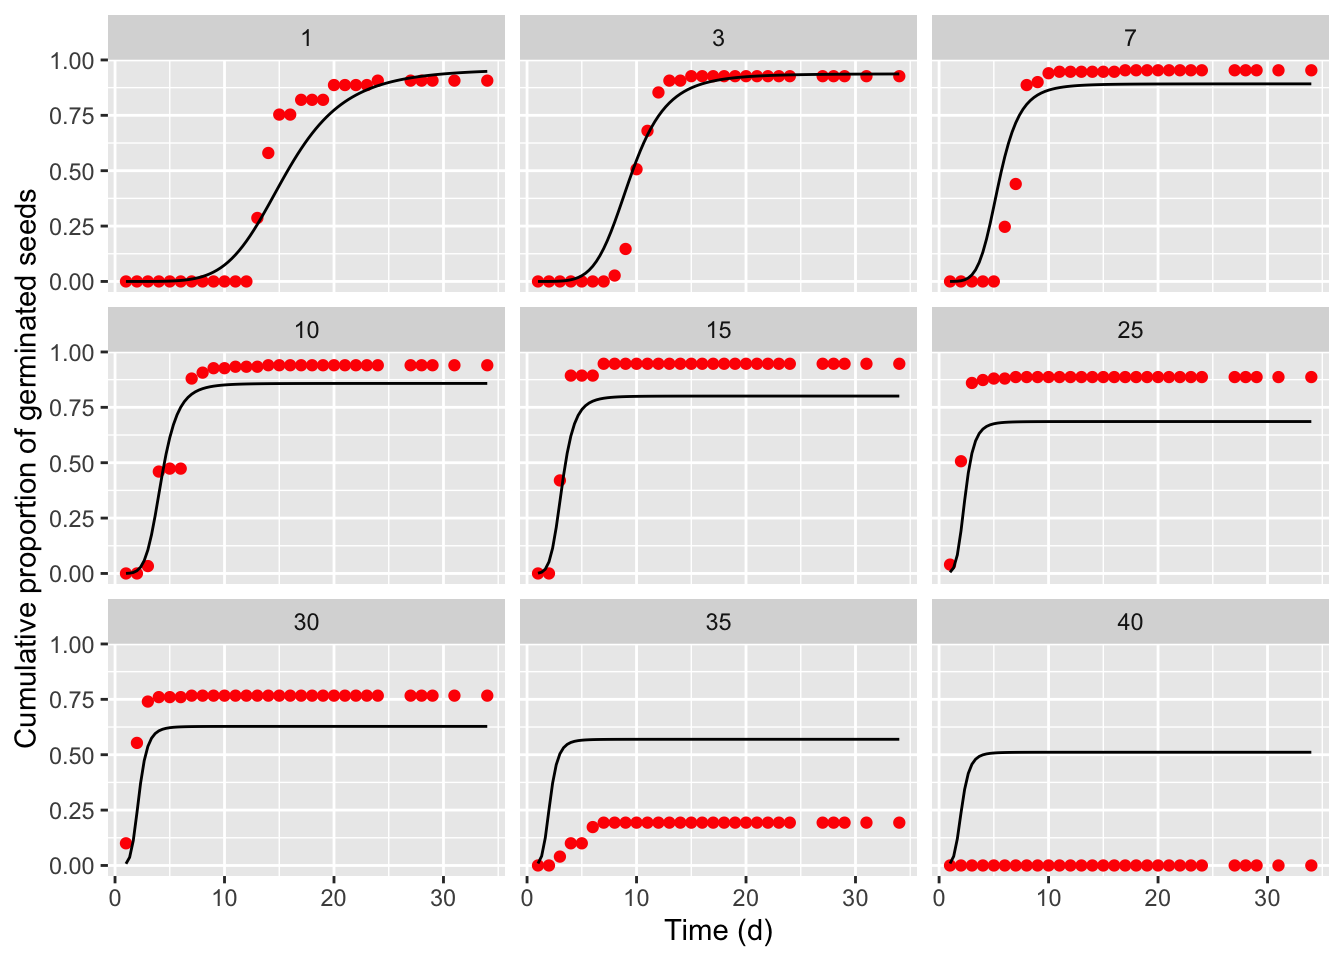
\includegraphics{_seedGerminationTutorial_files/figure-latex/unnamed-chunk-82-1.pdf}

The previous graph shows that the \texttt{TTEM()} model, that we had successfully used with other datasets, failed to provide an adequate description of the germination time-course for barley. Therefore, we modified one of the sub-models, by adopting the approach highlighted in Rowse and Finch-Savage (2003), where:

\[1/[e(T)] = GR_{50}(T) = \left\{ {\begin{array}{ll}
\frac{T - T_b}{\theta_T} & \textrm{if} \,\,\, T_b < T < T_d \\
\frac{T - T_b}{\theta_T} \left[ 1 - \frac{T - T_d}{T_c - T_d}  \right] & \textrm{if} \,\,\, T_d < T < T_c \\
0 & \textrm{if} \,\,\, T \leq T_b \,\,\, or \,\,\, T \geq T_c
\end{array}} \right. \]

Furthermore, we also made a further improvement, by coding another model where also the \(b\) parameter was allowed to change with temperature, according to the following equation:

\[ \sigma(T) = \frac{1}{b(T)} = \frac{1}{b_0} + s (T - T_b)\]

These two improved models were coded as the \texttt{TTERF()} function (with the only change in the `e' submodel), and as the \texttt{TTERFc()} function (with a change in both the `b' and `e' submodels), which are available within the \texttt{drcSeedGerm} package. The code below is used to fit both models and explore the resulting fits: the symbols show the observed means, the blue line represents the `TTERF' fit and the red line represents the `TTERFc' fit.

\begin{Shaded}
\begin{Highlighting}[]
\NormalTok{modTTERF }\OtherTok{\textless{}{-}} \FunctionTok{drmte}\NormalTok{( nSeeds }\SpecialCharTok{\textasciitilde{}}\NormalTok{ timeBef }\SpecialCharTok{+}\NormalTok{ timeAf }\SpecialCharTok{+}\NormalTok{ Temp, }\AttributeTok{data=}\NormalTok{barley,}
               \AttributeTok{fct=}\FunctionTok{TTERF}\NormalTok{())}
\NormalTok{modTTERFc }\OtherTok{\textless{}{-}} \FunctionTok{drmte}\NormalTok{(nSeeds }\SpecialCharTok{\textasciitilde{}}\NormalTok{ timeBef }\SpecialCharTok{+}\NormalTok{ timeAf }\SpecialCharTok{+}\NormalTok{ Temp, }\AttributeTok{data=}\NormalTok{barley,}
               \AttributeTok{fct=}\FunctionTok{TTERFc}\NormalTok{())}
\FunctionTok{AIC}\NormalTok{(modTTEM, modTTERF, modTTERFc)}
\DocumentationTok{\#\#            df      AIC}
\DocumentationTok{\#\# modTTEM   804 6478.917}
\DocumentationTok{\#\# modTTERF  803 5730.622}
\DocumentationTok{\#\# modTTERFc 802 5602.532}
\NormalTok{tab2 }\OtherTok{\textless{}{-}} \FunctionTok{plotData}\NormalTok{(modTTERF)}
\NormalTok{tab3 }\OtherTok{\textless{}{-}} \FunctionTok{plotData}\NormalTok{(modTTERFc)}

\FunctionTok{ggplot}\NormalTok{() }\SpecialCharTok{+}
  \FunctionTok{geom\_point}\NormalTok{(}\AttributeTok{data =}\NormalTok{ tab}\SpecialCharTok{$}\NormalTok{plotPoints, }\AttributeTok{mapping =} \FunctionTok{aes}\NormalTok{(}\AttributeTok{x =}\NormalTok{ timeAf, }\AttributeTok{y =}\NormalTok{ CDF),}
            \AttributeTok{col =} \StringTok{"red"}\NormalTok{) }\SpecialCharTok{+}
  \FunctionTok{geom\_line}\NormalTok{(}\AttributeTok{data =}\NormalTok{ tab2}\SpecialCharTok{$}\NormalTok{plotFits, }\AttributeTok{mapping =} \FunctionTok{aes}\NormalTok{(}\AttributeTok{x =}\NormalTok{ timeAf, }\AttributeTok{y =}\NormalTok{ CDF),}
            \AttributeTok{col =} \StringTok{"blue"}\NormalTok{) }\SpecialCharTok{+}
  \FunctionTok{geom\_line}\NormalTok{(}\AttributeTok{data =}\NormalTok{ tab3}\SpecialCharTok{$}\NormalTok{plotFits, }\AttributeTok{mapping =} \FunctionTok{aes}\NormalTok{(}\AttributeTok{x =}\NormalTok{ timeAf, }\AttributeTok{y =}\NormalTok{ CDF),}
            \AttributeTok{col =} \StringTok{"red"}\NormalTok{) }\SpecialCharTok{+}
  \FunctionTok{facet\_wrap}\NormalTok{( }\SpecialCharTok{\textasciitilde{}}\NormalTok{ Temp) }\SpecialCharTok{+}
  \FunctionTok{scale\_x\_continuous}\NormalTok{(}\AttributeTok{name =} \StringTok{"Time (d)"}\NormalTok{) }\SpecialCharTok{+}
  \FunctionTok{scale\_y\_continuous}\NormalTok{(}\AttributeTok{name =} \StringTok{"Cumulative proportion of germinated seeds"}\NormalTok{)}
\end{Highlighting}
\end{Shaded}

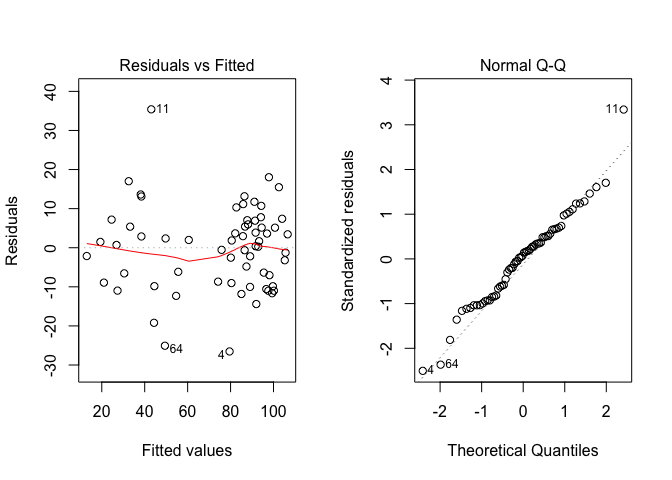
\includegraphics{_seedGerminationTutorial_files/figure-latex/unnamed-chunk-83-1.pdf}

We see that, with respect to the TTEM model, both the two improved models provide a better fit.

It should be clear that this modelling approach is rather flexible, by appropriately changing one or more submodels, and it can fit the germination pattern of several species in several environmental conditions.

\hypertarget{references}{%
\chapter{References}\label{references}}

\begin{enumerate}
\def\labelenumi{\arabic{enumi}.}
\tightlist
\item
  Barreiro-Ures D, Francisco-Fernández M, Cao R, Fraguela BB, Doallo R, González-Andújar JL, Reyes M (2019) Analysis of interval-grouped data in weed science: The binnednp Rcpp package. Ecol Evol 9:10903--10915
\item
  Bradford KJ (2002) Applications of hydrothermal time to quantifying and modeling seed germination and dormancy. Weed Sci 50:248--260
\item
  Brown, RF, DG Mayer (1988a) Representing Cumulative Germination. 1. A Critical Analysis of Single-value Germination Indices. Annals of Botany 61:117--125
\item
  Brown, RF, DG Mayer (1988b) Representing Cumulative Germination.: 2. The Use of the Weibull Function and Other Empirically Derived Curves. Annals of Botany 61:127--138
\item
  Catara, S., Cristaudo, A., Gualtieri, A., Galesi, R., Impelluso, C., Onofri, A. (2016). Threshold temperatures for seed germination in nine species of Verbascum (Scrophulariaceae). Seed Science Research 26, 30--46.
\item
  Davison, A.C., Hinkley, D.V. (1997). Bootstrap methods and their application. Cambridge University Press, UK.
\item
  Dutang, C, Goulet V and M. Pigeon (2008). actuar: An R Package for Actuarial Science. Journal of Statistical Software, vol.~25, no. 7, 1-37.
\item
  Fay, MP, PA Shaw (2010) Exact and Asymptotic Weighted Logrank Tests for Interval Censored Data: The interval R Package. Journal of Statistical Software 36:1--34
\item
  Gresta, F, G Avola, A Onofri, U Anastasi, A Cristaudo (2011) When Does Hard Coat Impose Dormancy in Legume Seeds? Lotus and Scorpiurus Case Study. Crop Science 51:1739--1747
\item
  Keshtkar E, Kudsk P, Mesgaran MB (2021) Perspective: Common errors in dose--response analysis and how to avoid them. Pest Manag Sci 77:2599--2608
\item
  Mesgaran, M.B., Mashhadi, H.R., Alizadeh, H., Hunt, J., Young, K.R., Cousens, R.D., 2013. Importance of distribution function selection for hydrothermal time models of seed germination. Weed Research 53, 89--101. \url{https://doi.org/10.1111/wre.12008}
\item
  Michael P. Fay, Pamela A. Shaw (2010). Exact and Asymptotic Weighted Logrank Tests for Interval Censored Data: The interval R Package. Journal of Statistical Software, 36(2), 1-34. URL \url{https://www.jstatsoft.org/v36/i02/}.
\item
  Onofri, A, F Gresta, F Tei (2010) A new method for the analysis of germination and emergence data of weed species. Weed Research 50:187--198
\item
  Onofri, A, MB Mesgaran, F Tei, RD Cousens (2011) The cure model: an improved way to describe seed germination? Weed Research 51:516--524
\item
  Onofri, A, MB Mesgaran, P Neve, RD Cousens (2014) Experimental design and parameter estimation for threshold models in seed germination. Weed Research 54:425--435
\item
  Onofri, A., Benincasa, P., Mesgaran, M.B., Ritz, C. (2018). Hydrothermal-time-to-event models for seed germination. European Journal of Agronomy 101, 129--139.
\item
  Onofri, A., Mesgaran, M., \& Ritz, C. (2022). A unified framework for the analysis of germination, emergence, and other time-to-event data in weed science. Weed Science, 1-13. \url{doi:10.1017/wsc.2022.8}
\item
  Onofri, Andrea, Hans Peter Piepho, and Marcin Kozak (2019). Analysing Censored Data in Agricultural Research: A Review with Examples and Software Tips. Annals of Applied Biology, 174, 3-13.
\item
  Onofri, Andrea, Paolo Benincasa, M B Mesgaran, and Christian Ritz (2018). Hydrothermal-Time-to-Event Models for Seed Germination. European Journal of Agronomy 101: 129--39.
\item
  Pace, R., Benincasa, P., Ghanem, M.E., Quinet, M., Lutts, S. (2012). Germination of untreated and primed seeds in rapeseed (brassica napus var oleifera del.) under salinity and low matric potential. Experimental Agriculture 48, 238--251.
\item
  Ritz C, Jensen SM, Gerhard D, Streibig JC (2019). Dose-response analysis using R CRC Press. USA
\item
  Ritz, C., Baty, F., Streibig, J. C., Gerhard, D. (2015). Dose-Response Analysis Using R PLOS ONE, 10(12)
\item
  Therneau T (2021). \emph{A Package for Survival Analysis in R}. R package version 3.2-11, \textless URL: \url{https://CRAN.R-project.org/package=survival}\textgreater.
\item
  Wickham, H, G Grolemund (2016) R for data science: import, tidy, transform, visualize, and model data. First edition. Sebastopol, CA: O'Reilly. 492 pp.
\item
  Yu, B., Peng, Y. (2008). Mixture cure models for multivariate survival data. Computational Statistics and Data Analysis 52, 1524--1532.
\item
  Zeileis, A., Köll, S., Graham, N. (2020). Various Versatile Variances: An Object-Oriented Implementation of Clustered Covariances in R. J. Stat. Soft. 95. \url{https://doi.org/10.18637/jss.v095.i01}
\item
  Alvarado, V., Bradford, K.J., 2002. A hydrothermal time model explains the cardinal temperatures for seed germination. Plant, Cell and Environment 25, 1061--1069.
\item
  Baty, F., Ritz, C., Charles, S., Brutsche, M., Flandrois, J. P., Delignette-Muller, M.-L., 2014. A toolbox for nonlinear regression in R: the package nlstools. Journal of Statistical Software, 65, 5, 1-21.
\item
  Bradford, K.J., 2002. Applications of hydrothermal time to quantifying and modelling seed germination and dormancy. Weed Science 50, 248--260.
\item
  Catara, S., Cristaudo, A., Gualtieri, A., Galesi, R., Impelluso, C., Onofri, A., 2016. Threshold temperatures for seed germination in nine species of Verbascum (Scrophulariaceae). Seed Science Research 26, 30--46.
\item
  Garcia-Huidobro, J., Monteith, J.L., Squire, R., 1982. Time, temperature and germination of pearl millet (\emph{Pennisetum typhoides} S \& H.). 1. Constant temperatures. Journal of Experimental Botany 33, 288--296.
\item
  Kropff, M.J., van Laar, H.H. 1993. Modelling crop-weed interactions. CAB International, Books.
\item
  Masin, R., Onofri, A., Gasparini, V., Zanin, G., 2017. Can alternating temperatures be used to estimate base temperature for seed germination? Weed Research 57, 390--398.
\item
  Onofri, A., Benincasa, P., Mesgaran, M.B., Ritz, C., 2018. Hydrothermal-time-to-event models for seed germination. European Journal of Agronomy 101, 129--139.
\item
  Ritz, C., Jensen, S. M., Gerhard, D., Streibig, J. C., 2019. Dose-Response Analysis Using R. CRC Press
\item
  Rowse, H.R., Finch-Savage, W.E., 2003. Hydrothermal threshold models can describe the germination response of carrot (Daucus carota) and onion (Allium cepa) seed populations across both sub- and supra-optimal temperatures. New Phytologist 158, 101--108.
\item
  Zeileis, A., 2006. Object-oriented computation of sandwich estimators. Journal of Statistical Software, 16, 9, 1-16.
\end{enumerate}

  \bibliography{drcSeedGerm.bib}

\end{document}
